% Dissertation Andreas Hill, Version 1.0
% 2. LaTeX Vorlage von Kai Husmann, Version 2.0
% 1. LaTeX Vorlage von Nikolas von L�pke, Version 1.1
%==================================================================================================================%
% Textencoding: 8859-1
\documentclass[
a4paper,
10pt,
titlepage,
%tablecaptionabove,
twoside,
openany,
%pointlessnumbers,
%fleqn, 
bibtotoc,
headings=twolinechapter,
headinclude]{scrbook}

%============================================ Load Packages ========================================================%

% required for mapping-article:
\usepackage{boldline}

%% required for JStatSoft:
\usepackage{Sweave}
\usepackage{latexsym}
\usepackage{a4}
\usepackage{epsfig}
\usepackage{flafter}
\usepackage{bm}
\usepackage{setspace}

%% captions
\usepackage[font=footnotesize]{caption}
\usepackage[font=footnotesize]{subcaption}

%% - create hyperlinks within the document
\usepackage{hyperref}
%\usepackage[pdfauthor={Andreas Hill}, pdftitle={Dissertation, Andreas Hill}]{hyperref}

%% - colors
\usepackage{color}
% \definecolor{link}{rgb}{0.45,0.51,0.67} % Dark blue colour for all links

%% - Serifenschriftart in �berschriften
\usepackage{lmodern}
\addtokomafont{disposition}{\rmfamily}

%% - Deutsche Anpassungen
\usepackage[ngerman,british]{babel}
\usepackage[T1]{fontenc}
\usepackage[latin1]{inputenc}
\usepackage{eurosym}

%% - bibliography
\usepackage{natbib}
\usepackage{apalike}
\hypersetup{
	colorlinks=true,
	linkcolor=black,
	citecolor=black,
	filecolor=magenta,      
	urlcolor=black}
\usepackage{multibib}
\usepackage{url}

%% - Sch�nere Tablellen
\usepackage{booktabs}
\usepackage{tabularx}
\usepackage{multirow}
\usepackage{graphicx} %Mit diesem package k�nnen pdf,png und jpg Graphiken eingelesen werden und direkt pdfs erzeugt werden
%\usepackage{picins}
%\usepackage{subfig}
%\usepackage{subfigure}
%% - Packages for Headings
\usepackage{fancyhdr}

%% - Packages f�r korrekte Einheiten:
\usepackage[squaren]{SIunits}
\usepackage[dvips]{rotating}
\usepackage{pdfpages}

%% - Packages f�r Formeln
\usepackage{amsmath}
\usepackage{amsthm}
\usepackage{amsfonts}
\usepackage{amssymb}
%\usepackage{mathptmx}

%% - Packages f�r Pseudocode
\usepackage[linesnumbered, algochapter]{algorithm2e}
\usepackage{enumerate}

%% - Paket f�r Grafik
\usepackage{tikz}
\usetikzlibrary{shapes,arrows,calc,positioning,shapes.geometric}
\usetikzlibrary{external}       % function to externalize tics-graphic buildings
\tikzset{external/force remake} % overwrites existing externalized pdfs
\tikzexternalize[prefix=cache/] % All externalized pdf are saved in folder 'cache'
\tikzexternaldisable % Only externalise on-demand

%% - Package f�r Zeilennummerierung
\usepackage{lineno}
%\linenumbers % uncomment for adding line numbers

%% - Querformat f�r den Anhang
\usepackage{array}

%% - f�r Abk�rzungsverzeichnis
\usepackage{acronym} 

%% - sonstige
\usepackage{chapterbib}
\usepackage{float}

%============================================ Define Settings ========================================================%

\pagestyle{fancy}

%% - Absatzformatierung
\setlength{\parindent}{0.5cm}
%\setlength{\parskip}{1.0ex plus 1.0ex minus 0.5ex}
%\setlength{\parskip}{6pt}%Abstand nach Absatz
\RequirePackage{setspace}
\setstretch{1.05}
\typearea[1.5cm]{15}

%% Platz an Seitenr�ndern
\usepackage{geometry}
\geometry{
	bottom=40mm,
	left=30mm,
	right=30mm
	,bindingoffset=0mm
}


% customize dictum format:
\setkomafont{dictumtext}{\itshape\small}
\setkomafont{dictumauthor}{\normalfont}
\renewcommand*\dictumwidth{\linewidth}
\renewcommand*\dictumauthorformat[1]{--- #1}
\renewcommand*\dictumrule{}

% own commands:
\newcommand{\adjrsq}{adjusted $R^2$}
\newcommand{\rmsecv}{RMSE$_{cv}$}
\newcommand{\mha}{m$^3$/ha}
\newcommand{\bwi}{BWI3}
\newcommand{\psynth}{PSYNTH}
\newcommand{\psmall}{PSMALL}
\newcommand{\extpsynth}{EXTPSYNTH}
\newcommand{\meanheight}{\textit{meanheight}}
\newcommand{\stddev}{\textit{stddev}}
\newcommand{\treespecies}{\textit{treespecies}}
\newcommand{\alsyear}{\textit{ALSyear}}


\definecolor{mygreen}{rgb}{0.1, 0.6, 0.4}
%\newcommand{\added}[1]{\color{mygreen}{#1} \color{black}}
%\newcommand{\changed}[1]{\color{red}{#1} \color{black}}
\newcommand{\added}[1]{\color{black}{#1} \color{black}}
\newcommand{\changed}[1]{\color{black}{#1} \color{black}}


\addtolength{\headwidth}{\marginparsep}
\addtolength{\headwidth}{\marginparwidth}

%============================================ Stat-Journal specific styles =========================================%

\newcommand{\proglang}[1]{\textit{#1}}
\newcommand{\pkg}[1]{{\fontseries{b}\selectfont #1}}
\newcommand{\code}[1]{\texttt{#1}}
\newcommand{\R}{R}
\newcommand{\var}{\mathbb{V}}
\newcommand{\EX}{\mathbb{E}}


% Text formatting --------------------------------------------------------------

%\newcommand{\R}{R}
%\newcommand{\address}[1]{\addvspace{\baselineskip}\noindent\emph{#1}}
%\newcommand{\email}[1]{\href{mailto:#1}{\normalfont\texttt{#1}}}
%
%\DeclareRobustCommand\code{\bgroup\@noligs\@codex}
%\def\@codex#1{\texorpdfstring%
%	{{\normalfont\ttfamily\hyphenchar\font=-1 #1}}%
%	{#1}\egroup}
%\newcommand{\kbd}[1]{{\normalfont\texttt{#1}}}
%\newcommand{\key}[1]{{\normalfont\texttt{\uppercase{#1}}}}
%\DeclareRobustCommand\samp{`\bgroup\@noligs\@sampx}
%\def\@sampx#1{{\normalfont\texttt{#1}}\egroup'}
%\newcommand{\var}[1]{{\normalfont\textsl{#1}}}
%\let\env=\code
%\newcommand{\file}[1]{{`\normalfont\textsf{#1}'}}
%\let\command=\code
%\let\option=\samp
%\newcommand{\dfn}[1]{{\normalfont\textsl{#1}}}
%% \acronym is effectively disabled since not used consistently
%\newcommand{\strong}[1]{\texorpdfstring%
%	{{\normalfont\fontseries{b}\selectfont #1}}%
%	{#1}}
%\let\pkg=\strong
%\let\proglong=\strong
%\newcommand{\CRANpkg}[1]{\href{https://CRAN.R-project.org/package=#1}{\pkg{#1}}}%
%\let\cpkg=\CRANpkg
%\newcommand{\ctv}[1]{\href{https://CRAN.R-project.org/view=#1}{\emph{#1}}}
%\newcommand{\BIOpkg}[1]{\href{http://www.bioconductor.org/packages/release/bioc/html/#1.html}{\pkg{#1}}}

% Example environments ---------------------------------------------------------
\RequirePackage{fancyvrb}
\RequirePackage{alltt}

\DefineVerbatimEnvironment{example}{Verbatim}{}
\renewenvironment{example*}{\begin{alltt}}{\end{alltt}}

% Support for output from Sweave, and generic session style code
% These used to have fontshape=sl for Sinput/Scode/Sin, but pslatex
% won't use a condensed font in that case.

% Update (2015-05-28 by DS): remove fontsize=\small to match example environment

\DefineVerbatimEnvironment{Sinput}{Verbatim}{}
\DefineVerbatimEnvironment{Soutput}{Verbatim}{}
\DefineVerbatimEnvironment{Scode}{Verbatim}{}
\DefineVerbatimEnvironment{Sin}{Verbatim}{}
\DefineVerbatimEnvironment{Sout}{Verbatim}{}
%\newenvironment{Schunk}{}{}

%============================================ END Stat-Journal specific styles ===================================%



%===================================================================================================================%
%============================================ Start Document =======================================================%
\begin{document}
	
%% ------------------------------ Deckblatt -------------------------------------- %%
	\thispagestyle{empty}
	
%%%%%%%%%%%%%%%
%% Deckblatt %%
%%%%%%%%%%%%%%%

\begin{titlepage}

\begin{center}

%\vspace*{1cm}
\textsc{DISS. ETH NO. .............}

\vspace*{2cm}
\Large
\textbf{Integration of Small Area Estimation Procedures of Timber Volume Resources in Large Scale Forest Inventories}

\vspace*{1cm}
A dissertation submitted to the \\
ETH ZURICH

\vspace*{1cm}
for the degree of \\
Doctor of Sciences

\vspace*{1cm}
presented by

\vspace*{0.5cm}
\textsc{Andreas Christian Hill} \\
MSc. of Sciences

\vspace*{0.5cm}
born 15 January 1986 \\
citizen of Germany

\vspace*{1cm}
accepted on the recommendation of

\vspace*{0.2cm}
Prof. Dr. H.R. Heinimann, examiner\\
PD Dr. D. Mandallaz, supervisor, co-examiner\\
Prof. Dr. J. Saborowski, co-examiner\\
Dr. J. Breidenbach, co-examiner

\vspace{3cm}
Zurich, 2018


\end{center}

\end{titlepage}
	%\pagestyle{empty}
	%\cleardoublepage
	
%% ------------------------------ Referees -------------------------------------- %%	
	%
\vspace*{\fill}

\begin{tabular}{lll}
1. Gutachter:& Prof. Dr. J�rgen Nagel\\
2. Gutachter:& Prof. Dr. Bernhard M�hring\\
\end{tabular}

\begin{tabular}{lll}
Tag der m�ndlichen Pr�fung:& 17. Oktober 2017 \\
\end{tabular}

	%\pagestyle{empty}
	%\cleardoublepage
	%\thispagestyle{empty}
	%\newpage
	%\thispagestyle{empty}
	%\mbox{}
	\pagebreak
	%\pagenumbering{arabic}
	
%% ------------------------------ Table of Contents -------------------------------------- %%
	\pagenumbering{roman}
	%\begin{otherlanguage}{ngerman}
\chapter*{Zusammenfassung}
\label{chap:Zusammenfassung}
\addcontentsline{toc}{chapter}{Zusammenfassung}

Das Ziel dieser Dissertation war es, Methoden für die Einbindung von Hilfsinformation aus Fernerkundungsdaten in bestehende Waldinventuren beizutragen. Unter speziellem Fokus auf die praktischen Implementierung und Anwendung stand die Frage im Vordergrund, ob durch Kombination mit Hilfsinformationen terrestrische Daten aus grossräumigen Nationalinventuren auch für Schätzungen mit akzeptablen Genauigkeiten auf deutlich kleinräumigeren Ebenen verwendet werden können. Dies wurde im Rahmen zweier Ansätze für Kleingebietsschätzungen näher untersucht.\par

Der erste Ansatz bestand aus der Anwendung design-basierter Regressionsschätzer für Kleingebietsschätzungen und wurde in einer Studie im Bundesland Rheinland-Pfalz (Deutschland) getestet. Zunächst wurde das bestehende Netz der Nationalen Waldinventur zu einem zweiphasigen Stichprobendesign erweitert. Anschliessend wurden durch die Kombination mit landesweit vorhandenen Fernerkundungsdaten Schätzung der Holzvorräte auf Forstamt- und Forstrevierebene berechnet und die erreichten Schätzgenauigkeiten evaluiert. Die Ergebnisse der Studie werden in drei aufeinanderfolgenden Kapitel vorgestellt: Das erste Kapitel gibt einen umfassenden Überblick über design-basierte Regressionsschätzer mit speziellem Fokus auf Kleingebietschätzungen und erläutert deren Implementierung in ein statistisches Softwarepaket welches im Rahmen der Studie entwickelt wurde. Im zweiten Kapitel wird auf die drei grössten Herausforderungen bei der Regressionsmodellierung eingegangen. Zu diesen Herausforderungen zählten der zeitliche Versatz von terrestrischen Aufnahmen und Erhebung der Fernerkundunsgdaten, die optimale Ableitung erklärender Variablen unter unbekannter räumlicher Ausdehnung der terrestrisch durchgeführten Aufnahme (Winkelzählprobe), und die Verwendung von Baumarteninformation aus Satellitenbildklassifikation als zusätzliche erklärende Variable. Das dritte Kapitel illustriert die Durchführung der Kleingebietschätzungen als Synthese aus Kapitel 1 und 2, und präsentiert einen Vergleich der erzielten Schätzgenauigkeiten mit jenen, welche sich unter ausschliesslicher Benutzung der terrestrischen Inventurdaten (einphasige Schätzung) ergeben. Es zeigte sich, dass durch Anwendung der Kleingebietsschätzer die Varianz der einphasigen Schätzung im Mittel um 43\% und 25\% auf Forstamt- und Revierebene reduziert werden konnte, was zu mittleren Schätzfehlern von 5\% und 11\% führte. Damit untermauern diese Resultate das grosse Potential von design-basierten Kleingebietsschätzern für die Verwendung von Nationalinventurdaten auf kleinräumigen Managementebenen. Zudem zeigte sich, dass Zeitdifferenzen zwischen terrestrischen- und Fernerkundungsdaten zu einer Verschlechterung der Modellgenauigkeit führen. Dieser Effekt konnte jedoch durch die Verwendung des Aufnahmedatums als kategorielle Variable im Regressionsmodell deutlich verringert werden. Auch führte neben der Vegetationshöheninformation die zusätzliche Verwendung der geschätzten Hauptbaumart eines Stichprobenpunktes zu einer Verbesserung der Modellgenauigkeit. Durch die Anwendung eines Kalibrierungsmodelles war es zudem möglich, die negativen Effekte von Fehlklassifikationen der Baumarten auf das Regressionsmodell zu neutralisieren. Die Einbeziehung der kategoriellen erklärenden Variablen im Regressionsmodell erweiterte dabei den gewählten Ansatz zu Post-Stratifizierung, welches ein bekanntes und effizientes Mittel zur Varianzreduktion von Schätzungen darstellt.\par

Der zweite Ansatz Bestand aus der Anwendung eines modelabhängigen Mapping-Verfahrens, in welchem der Flächenbezug der Modellprognosen (Pixel der Vorhersagekarte) der räumlichen Ausdehnung eines Stichprobenkreises entspricht. Damit solche räumlich hochaufgelösten Prognosekarten zur Lokation von forstlichen Eingriffen auf kleinräumigsten Ebenen benutzt werden können, ist der Anspruch an ihre Genauigkeit hoch. Daher war es Ziel, für Prognosekarten kontinuierlicher Waldattribute eine zusätzliche Methode zur Bereitstellung der Genauigkeit pro Kartenpixel zu testen. Dies wurde durch die Berechnung der Nutzergenauigkeit, welche für die Genauigkeitsanalyse von Klassifikationen angewendet wird, für definierte Prognoseintervalle realisiert. In diesem Rahmen wurde auch ein Optimierungsalgorithmus getestet, welcher die Spannweite der Prognosen automatisch in kleinstmögliche Intervalle mit grösstmöglichen Nutzergenauigkeiten einteilt. Die Methoden wurden in einem subalpinen Testgebiet in der Schweiz am Beispiel einer Holzvorratskarte getestet. Daten der kantonalen Waldinventur dienten dabei als Referenzdaten um die Genauigkeit der Prognosekarte zu validieren. Die Ergebnisse deuten an, dass die Vorhersagefehler einzelner Wertebereiche oft deutlich höher sind als auf Basis von generalisierenden Kriterien der Modellgenauigkeit vermutet werden kann. Die vorgeschlagene Validierungsmethode bietet daher eine zusätzliche Genauigkeitsangabe, welche einfach berechnet werden kann und die Information bezüglich der Kartengenauigkeit verbessert. Die Optimierungsmethode kann dazu benutzt werden, eine Prognosekarte in Wertebereiche variabler Länge einzuteilen, welche die zugrundeliegende Modellgenauigkeit reflektieren.

\end{otherlanguage}




	%\input{Abstract}
	%% Inhaltsverzeichnis %%%%%%%%%%%%%%%%%%%%%%%%%%%%%%%%%%%%%%%
	\setcounter{tocdepth}{1}
	\hypersetup{linkcolor=black}{ % Damit nicht das ganze TOC blau ist.
		\tableofcontents
	}
	\thispagestyle{plain}
	\newpage
	
%% ------------------------------ List of Figures -------------------------------------- %%
	\listoffigures
	\thispagestyle{plain}
	\newpage

%% ------------------------------ List of Tables -------------------------------------- %%
	\listoftables
	\pagestyle{plain}
	%\clearpage
	%\newpage
	%\mbox{}
	%\pagebreak
	%\thispagestyle{empty}
	
%% ------------------------------ Acknowledgements -------------------------------------- %%
\chapter*{Acknowledgements}

When I started my studies on forest sciences at the University of G{\"o}ttingen in 2006, I would never have imagined that my path would led me to Switzerland finishing a doctoral thesis on forest inventory methods at ETH Zurich. On my entire way, I had the great privilege to meet and be accompanied by many people who supported me, backed me up, shared my passion, sparked my interests on interesting subjects and also became very good friends. I would like to take this opportunity to thank those people from the bottom of my heart and express my deep gratitude.\par 

As having been trained in statistical thinking, I can provide strong further evidence against the hypothesis that the completion of a dissertation thesis is possible without the support of colleagues, friends and family. I particularly want to thank


\renewcommand{\labelitemi}{--}
\begin{itemize}
	\item Prof. Hans Rudolf Heinimann - for giving me the opportunity to continue my work in the field of forest inventory at his chair of Land Use Engineering at ETH Zurich, and giving me the freedom to follow my research interests and explore new ideas.
	
	\item Prof. em. Joachim Saborowski (University of G{\"o}ttingen) and Dr. Johannes Breidenbach (Norwegian Institute of Bioeconomy Research) for acting as co-examiners.
	
	\item Daniel Mandallaz (em. associate professor, ETH Zurich) - for being an excellent and reliable supervisor, for his guidance and always taking the time for questions and discussions, and for benefiting from his great experience in the field of statistics and forest inventory.
	
	\item Dr. Alexander Massey - for supporting my work with many helpful advice and criticism, and for collaboration and proofreading.
	
	\item Dr. Kai Husmann - for his help in many tasks and for countless interesting and constructive discussions concerning our scientific works - and even more for those not concerning it.
	
	\item My colleagues Jochen Breschan, Leo Bont, Daniel Tr{\"u}ssel, Franziska Baumgartner, Maja Messerli, Andreas Gabriel, Sabrina Maurer and the entire group of forest engineering at ETH Zurich for all their support and encouraging words, and for all the nice moments together.
	
	\item The forest service of Rhineland-Palatinate, particularly Dr. Joachim Langshausen, J{\"u}rgen Dietz and Claus-Andreas Lessander, for being a reliable partner, supporting practical questions, and for their openness to new methods and ideas.
	
	\item Peter Kruse (forest service of Rhineland-Palatinate) for sparking my interest on forestry 13 years ago.
	
	\item My family - my parents Elfie and Joachim, my brother Michael, my grandmother Klara, my parents-in-law Hildegard and Goswin, Andreas and Michael, Martina, Lore and Pauline for all their support and encouragement.
	
	\item Christina - for all her love and support, and having travelled this journey with me side-by-side.
	
\end{itemize}


\newpage

	\thispagestyle{plain}
	%\clearpage
	%\newpage
	%\mbox{}
	%\pagebreak
	%\thispagestyle{empty}
	\hypersetup{linkcolor=black}{} % Links wieder blau
	
%% ------------------------------ Summary -------------------------------------- %%
%\chapter*{Summary}
\label{chap:Summary}
\addcontentsline{toc}{chapter}{Summary}

The objective of this cumulative thesis was to contribute methods for incorporating auxiliary information, such as remote sensing data, in existing forest inventories. The overall focus of these methods were to increase the value of existing large scale inventories, which are usually characterised by low sampling frequencies, on small-scale management levels. This research question was investigated in two main studies.\par

The first study presented in this thesis focused on the application of latest design-based regression estimators for small area estimation. The objective of the study was to develop a double-sampling procedure for the German National Forest Inventory (NFI) and evaluate whether the implied combination of remote sensing data and the terrestrial NFI data can provide sufficient estimation precision on two small-scale management levels. The approach was applied by the example of timber volume estimation within two forest district levels in the German federal state of Rhineland-Palatinate. The work on this study is presented in three subsequent chapters: the first chapter gives a comprehensive review of model-assisted design-based small area regression estimators and demonstrates their implementation in a statistical software package that was developed for the purpose of this study. The second chapter addresses challenges that occurred during the identification of a suitable timber-volume regression model to be used in the estimators, i.e. 1) heterogeneity of the remote sensing data due to quality variations and time gaps to the terrestrial survey, 2) derivation of explanatory variables under angle count sampling, and 3) incorporation of tree species map information. The third chapter illustrates the implementation of the small area estimation procedure and evaluate its potential by comparing the estimation precisions to those derived under one-phase sampling, i.e. exclusively using the terrestrial NFI data available within each management unit. The major results were the following: it was demonstrated that on both management levels, the suggested double-sampling procedure was able to substantially reduce the estimation error compared to the standard one-phase approach. Additionally, post-stratification according to variables that reflect quality variations or temporal asynchronicity in the auxiliary information turned out to be an effective means to improve the precision of OLS regression models. The additional stratification to tree species led to a further improvement of model performance and suggests the use of such information in forthcoming inventories.\par

The second study was carried out in a model-dependent framework and investigated an alternative approach of deriving pixel-wise confidence intervals for forest attribute maps. The core approach was to use available inventory data for map validation by applying concepts of accuracy assessment usually known from evaluation of categorical classification results. The definition of intervals within the range of map predictions and their respective reference data were used to calculate the user's accuracies as the probability for each interval to reflect the ground truth. In this framework, an optimization algorithm was developed to automatically identify intervals that lead to optimal classification schemes. The method was tested on a timber volume map for a mountainous study site in Switzerland using data from the regional forest inventory as validation data. The results from the study suggested that resulting class accuracies can turn out to be substantially lower than overall model accuracy metrics such as $R^2$ or root mean square error might suggest. The validation method thus provides an additional accuracy metric that can be easily calculated and improves the information about the accuracy provided by forest attribute maps.


%	\thispagestyle{plain}
%	%\cleardoublepage
%\begin{otherlanguage}{ngerman}
\chapter*{Zusammenfassung}
\label{chap:Zusammenfassung}
\addcontentsline{toc}{chapter}{Zusammenfassung}

Das Ziel dieser Dissertation war es, Methoden für die Einbindung von Hilfsinformation aus Fernerkundungsdaten in bestehende Waldinventuren beizutragen. Unter speziellem Fokus auf die praktischen Implementierung und Anwendung stand die Frage im Vordergrund, ob durch Kombination mit Hilfsinformationen terrestrische Daten aus grossräumigen Nationalinventuren auch für Schätzungen mit akzeptablen Genauigkeiten auf deutlich kleinräumigeren Ebenen verwendet werden können. Dies wurde im Rahmen zweier Ansätze für Kleingebietsschätzungen näher untersucht.\par

Der erste Ansatz bestand aus der Anwendung design-basierter Regressionsschätzer für Kleingebietsschätzungen und wurde in einer Studie im Bundesland Rheinland-Pfalz (Deutschland) getestet. Zunächst wurde das bestehende Netz der Nationalen Waldinventur zu einem zweiphasigen Stichprobendesign erweitert. Anschliessend wurden durch die Kombination mit landesweit vorhandenen Fernerkundungsdaten Schätzung der Holzvorräte auf Forstamt- und Forstrevierebene berechnet und die erreichten Schätzgenauigkeiten evaluiert. Die Ergebnisse der Studie werden in drei aufeinanderfolgenden Kapitel vorgestellt: Das erste Kapitel gibt einen umfassenden Überblick über design-basierte Regressionsschätzer mit speziellem Fokus auf Kleingebietschätzungen und erläutert deren Implementierung in ein statistisches Softwarepaket welches im Rahmen der Studie entwickelt wurde. Im zweiten Kapitel wird auf die drei grössten Herausforderungen bei der Regressionsmodellierung eingegangen. Zu diesen Herausforderungen zählten der zeitliche Versatz von terrestrischen Aufnahmen und Erhebung der Fernerkundunsgdaten, die optimale Ableitung erklärender Variablen unter unbekannter räumlicher Ausdehnung der terrestrisch durchgeführten Aufnahme (Winkelzählprobe), und die Verwendung von Baumarteninformation aus Satellitenbildklassifikation als zusätzliche erklärende Variable. Das dritte Kapitel illustriert die Durchführung der Kleingebietschätzungen als Synthese aus Kapitel 1 und 2, und präsentiert einen Vergleich der erzielten Schätzgenauigkeiten mit jenen, welche sich unter ausschliesslicher Benutzung der terrestrischen Inventurdaten (einphasige Schätzung) ergeben. Es zeigte sich, dass durch Anwendung der Kleingebietsschätzer die Varianz der einphasigen Schätzung im Mittel um 43\% und 25\% auf Forstamt- und Revierebene reduziert werden konnte, was zu mittleren Schätzfehlern von 5\% und 11\% führte. Damit untermauern diese Resultate das grosse Potential von design-basierten Kleingebietsschätzern für die Verwendung von Nationalinventurdaten auf kleinräumigen Managementebenen. Zudem zeigte sich, dass Zeitdifferenzen zwischen terrestrischen- und Fernerkundungsdaten zu einer Verschlechterung der Modellgenauigkeit führen. Dieser Effekt konnte jedoch durch die Verwendung des Aufnahmedatums als kategorielle Variable im Regressionsmodell deutlich verringert werden. Auch führte neben der Vegetationshöheninformation die zusätzliche Verwendung der geschätzten Hauptbaumart eines Stichprobenpunktes zu einer Verbesserung der Modellgenauigkeit. Durch die Anwendung eines Kalibrierungsmodelles war es zudem möglich, die negativen Effekte von Fehlklassifikationen der Baumarten auf das Regressionsmodell zu neutralisieren. Die Einbeziehung der kategoriellen erklärenden Variablen im Regressionsmodell erweiterte dabei den gewählten Ansatz zu Post-Stratifizierung, welches ein bekanntes und effizientes Mittel zur Varianzreduktion von Schätzungen darstellt.\par

Der zweite Ansatz Bestand aus der Anwendung eines modelabhängigen Mapping-Verfahrens, in welchem der Flächenbezug der Modellprognosen (Pixel der Vorhersagekarte) der räumlichen Ausdehnung eines Stichprobenkreises entspricht. Damit solche räumlich hochaufgelösten Prognosekarten zur Lokation von forstlichen Eingriffen auf kleinräumigsten Ebenen benutzt werden können, ist der Anspruch an ihre Genauigkeit hoch. Daher war es Ziel, für Prognosekarten kontinuierlicher Waldattribute eine zusätzliche Methode zur Bereitstellung der Genauigkeit pro Kartenpixel zu testen. Dies wurde durch die Berechnung der Nutzergenauigkeit, welche für die Genauigkeitsanalyse von Klassifikationen angewendet wird, für definierte Prognoseintervalle realisiert. In diesem Rahmen wurde auch ein Optimierungsalgorithmus getestet, welcher die Spannweite der Prognosen automatisch in kleinstmögliche Intervalle mit grösstmöglichen Nutzergenauigkeiten einteilt. Die Methoden wurden in einem subalpinen Testgebiet in der Schweiz am Beispiel einer Holzvorratskarte getestet. Daten der kantonalen Waldinventur dienten dabei als Referenzdaten um die Genauigkeit der Prognosekarte zu validieren. Die Ergebnisse deuten an, dass die Vorhersagefehler einzelner Wertebereiche oft deutlich höher sind als auf Basis von generalisierenden Kriterien der Modellgenauigkeit vermutet werden kann. Die vorgeschlagene Validierungsmethode bietet daher eine zusätzliche Genauigkeitsangabe, welche einfach berechnet werden kann und die Information bezüglich der Kartengenauigkeit verbessert. Die Optimierungsmethode kann dazu benutzt werden, eine Prognosekarte in Wertebereiche variabler Länge einzuteilen, welche die zugrundeliegende Modellgenauigkeit reflektieren.

\end{otherlanguage}




%	%\cleardoublepage
%	\thispagestyle{plain}
%	\clearpage
%	\newpage
%	%\thispagestyle{empty}
%	\mbox{}
%	\pagebreak
%	\thispagestyle{empty}
%	
	%Definiert die L�nge der Kopfzeile
	% --> (L=Left, R=Right, E=Even (pagenumbers), O=Odd (page numbers)
	\pagestyle{fancy} \renewcommand{\headrulewidth}{0.4pt}
	\renewcommand{\headrulewidth}{0.4pt}
	\fancyhead{} \fancyfoot{}
	\setlength{\headheight}{30pt}
	\renewcommand{\chaptermark}[1]{ \markboth{\small\ \thechapter\ \hspace{1.5mm}\ #1}{} }   % \thechapter defines current chapter number
		\fancyhead[RO]{\leftmark} %  \leftmark defines current CHAPTER name (where to put \chaptermark)
	\renewcommand{\sectionmark}[1]{ \markright{\small \thesection\ \hspace{1.5mm}\  #1}{} }  % \thesection defines current section number
		\fancyhead[LE]{\rightmark} % \rightmark defines current SECTION name (where to put \sectionmark)
	\fancyfoot[LE]{\thepage} % \thepage defines current page number 
	\fancyfoot[RO]{\thepage}


%% ------------------------------ Introduction -------------------------------------------------------- %%	
\pagenumbering{arabic}
%\setchapterpreamble[uc][0.8\textwidth]{%
%	\dictum[George Bernard Shaw]{%
%		``It is the mark of a truly intelligent person to be moved by statistics.''}\vskip20em}
	
\setchapterpreamble[uc][0.8\textwidth]{%
			\dictum[George Bernard Shaw]{%
				``Science never solves a problem without creating ten more.''}\vskip20em}

%\setchapterpreamble[uc][0.8\textwidth]{%
%	\dictum[Han Solo]{%
%		``She may not look like much, but she's got it where it counts.''}\vskip20em}			
	

	
\chapter{General Introduction}
\label{chap:intro}
\newpage
%------------------------------------------------------------------------------------------------%
% ---------------------------- History and state of the art------------------------------------- %
\section{Short history of forest inventory}
\label{sec:intro:hist_soa}

%This first section has the objective to outline important developments in forest inventories that subsequently led to the recent state of methods to which this thesis was intended to contribute. 
The first known conductions of forest inventories date back to the 14th and 15th century. They looked quite different from today's inventories and exclusively comprised a visual inspection that was carried out by riding or walking through the forests. These inspections were a means to acquire a representative impression about the state of large forest areas as well as to determine spatial units for harvesting \citep{zoehrer1980}. Whereas these inspections constituted a response to already increasing wood shortages, the first reference to sustainable forest management in literature is only found two centuries later in the book \textit{Silviculatura Oeconomica} written by \citet{carlowitz1713}, who suggested concepts that besides reforestation mostly targeted at a 'continuous and sustainable' use of wood. However, these concepts required updated, profound and reliable information about the forested areas.\par

While the first use of sample plots to gather representative information about the state and development of forests date back to \citet{hartig1795}, major advancements of sample-based inventories came up at the beginning of the 20th century together with the development of statistical sampling methods. In North America, the first sample-based inventories (so-called \textit{timber cruises}) were conducted around 1930. The surveys were initially performed by visual assessments and later by a full census of all trees along systematically arranged lines. The idea of these so-called \textit{strip-sampling} inventories was to gather information only for a small percentage of the forest, and this information was then subsequently extrapolated to the entire forest area. In addition, the surveyed strips were also used to provide forest attribute maps. These strip sampling techniques were further developed by \citet{goodspeed1934} and \citet{langballe1938} who both proposed to collect information only within sample plots aligned with the strip lines (line-plot sampling) in substitution for a complete census within the stripes as a means to reduce costs and to make the cruises more efficient.\par 

In addition to improving the efficiency of sampling techniques, it also became of high importance to reliably quantify the estimation errors associated to estimated forest attributes. Solutions were developed in two mathematical frameworks of inference that rely on either randomization of the sampling process or sampling from an underlying stochastic process and are today known as the \textit{design-based} and \textit{model-dependent} approach. Randomization of the sample plot locations in order to allow for a valid estimate of the sampling error was first recommended by \citet{hasel1938}. A defining advancement in design-based survey sampling constituted the concept of unequal probability sampling by \citet{hansen1943}, who showed that using inclusion probabilities proportional to the value of the target attribute (so-called \textit{probability proportional to size} or \textit{PPS} sampling) could substantially increase estimation precision. An unbiased estimator for unequal probability sampling was then contributed by \citet{horvitz1952}. The concept of \textit{PPS} sampling is implemented in most of today's forest inventories by the use of concentric sample plots. A method which perfectly realizes PPS sampling is the angle-count sampling (ACS) technique introduced by Bitterlich in 1947 \citep{bitterlich1984}, and it was \citet{grosenbaugh1958} who related ACS to the probabilistic sampling theory. A further important development was the reformulation of the design-based estimation frame, in particular the Horwitz-Thompson estimator, within the \textit{infinite population approach} by \citet{mandallaz2008}, which provided a much better definition of the underlying population for forest inventories compared to design-based survey methods for finite populations as applied in official statistics \citep[e.g.]{sarndal2003}.\par

The huge advancements in the conduction of national forest inventories in the Nordic countries around 1920 considerably contributed to the development of estimators in the model-dependent framework, since these inventories used the concept of systematic strip sampling. Especially the variance estimators for systematic sampling by Mat\'{e}rn (1947, 1960) were used to quantify the estimation precisions \citep{kangas2006}. Even while Mat\'{e}rns variance estimators relied on modelling spatial trends, it was \citet{mandallaz1993} who first applied geospatial kriging techniques in the field of forest inventory.\par


%Since the 1950s, the demands on forest services have steadily been increasing. Beside the role of forests as wood supply, more diverse functions of forests became of importance, such as the recreational role, conservation of biodiversity, forest health and vitality (McRoberts et al. 2010) and also regulating and protective functions (Berger and Rey 2004; Frehner et al. 2005). As a result, today's forest inventories have to collect a huge amount of variables in order to provide quantitative data to report on each of these information needs. This has been supported by the development of a broad range of concepts and methods particularly suited to estimate forest inventory attributes \citep{gregoire2007, kohl2006, mandallaz2008, schreuder1993}. The large number of attributes to be collected has also further limited the number of sample plots than can be surveyed in a given amount of time, in particular under recent cost-restrictions. As a result, there has been an increasing need for alternative inventory methods that can maintain estimation precision at lower costs, i.e. fewer terrestrial sample sizes, or achieve higher estimation precision at identical costs \citep{vonluepke2013}. 
%
%A method which has been intensively used in this respect is multi-phase sampling. The core concept of such sampling procedures is to enlarge the sample size in order to gain higher estimation precision without enlarging the terrestrial sample size. This is done by using predictions of the target variable at additional sample locations where the terrestrial information has not been gathered. These predictions are generated by statistical models, commonly regression models, that use explanatory variables derived from auxiliary data. Regression estimators using this concept ususally use two samples of different sampling intensities (double- or two-phase sampling). According to \citet{schreuder1993}, double-sampling methods had already been developed by Cochran (1939), Neyman (1938) and Watson (1937) before they were extensively formulated in the forest inventory context by \citet{schreuder1993, kohl2006, gregoire2007, mandallaz2008}.
%
%Application of double-sampling methods in forestry became particularly interesting with the availablity of suitable auxiliary information. For a long time, this information was exclusively provided by aerial photographs. In Canada, aerial photographs had a long tradition and were already used in the 1930s in order to locate the inventory strips through merchantable forest stands. In Switzerland, Schmidt (1970) suggested a two-phase method where tree heights, stand densities, crown diameters and stem numbers are determined by a visual interpretation of aerial photos, and the terrestrial inventory is carried out only at a subsample. This method was then indeed implemented in the first Swiss NFI in 1983. Also Zöhrer (1980) in Germany already stated the use of areal photographs as a state-of-the-art of modern forest inventories. He described a comprehensive catalog of forest attributes to be derived from aerial photo interpretation, amongst others tree species, crown diameter, tree heigths as well as timber volume estimates on tree and stand level. He also suggested to use the resulting forest attribute maps for forest inventories in terms of building strata of different sampling frequencies.

% Major advancements in the incorporation of auxiliary data in forest inventory however emerged with a) the availability of large-scale remote sensing data technologies and b) increased computation capacities that allowed for automatically deriving information from that sources.

% Particularly the availability of small-footprint airborne laserscanning data 



% Recently, \citet{mandallaz2013c} and \citet{vonLuepke2012} extended double-sampling to triple-sampling and provided regression estimators that can use auxiliary information derived at two different sampling intensities.


%
%
%
%
%
%
%
%
%
%
%
%
%
%
%
%
%
%
%
%
%
%
%






























%%This first section has the objective to outline important developments in forest inventories that subsequently led to the recent state of methods to which this thesis was intended to contribute. 
%The first known conductions of forest inventories date back to the 14th and 15th century. They looked quite different from today's inventories and exclusively comprised a visual inspection that was carried out by riding or walking through the forest. These inspections were a means to acquire a representative impression about the state of large forest areas as well as to determine spatial units for harvesting \citep{zoehrer1980}. The ability to estimate forest attributes by eye remained a crucial ability of forest practicioners for the next five centuries and is today still applied for stand inventories in many countries. Whereas these inspections constituted a response to increasing wood shortages, the first reference to sustainable forest management in literature is only found two centuries later in the book \textit{Silviculatura Oeconomica} written by \citet{carlowitz1713}. With the objective of a 'continuous and sustainable usage', Carlowitz suggested concepts that besides reforstation mostly targeted a more efficient use of wood.\par
%
%While the first use of sample plots to gather representative information date back to \citet{hartig1795}, major advancements of sample-based inventories came up at the beginning of the 20th century together with the development of statistical sampling methods. In North America, the first sample-based inventories (so-called \textit{timber cruises}) were conducted around 1930. The surveys were initially performed by visual assessment and later by a full census of all trees along systematically arranged lines. The idea of these so-called \textit{strip-sampling} inventories was to gather information only for a small percentage of the forest, which was then subsequently extrapolated to the entire forest area. The use of strips was at the same time also a means to produce forest attribute maps. An important further development of this sampling technique was the work of \citet{goodspeed1934} who advocated the collection of data within sample plots aligned with the strip lines (line-plot sampling) in substitution for a complete census within the stripes in order to improve the efficiency of the cruises. At the same time, \citet{langballe1938} demonstrated an early two-stage sampling approach in Canada in order to further reduce costs of a terrestrial cruise. They were confronted with considerable increases in survey costs triggered by stands becoming smaller, which required closer line spacing and more plots surveyed in the cruise. They thus proposed a method where field crews quickly counted the trees within each strip by eye, whereas they only performed time-consuming measurements at few plots within the strip. They subsequently used the relationship between the target variable (basal area) and the counted stem number to extrapolate the plot measurements to the entire strip area. This concept can be regarded as an early version of modern two-phase or two-stage estimation techniques.\par 
%
%Beside improving the efficiency, an issue that also became of high importance was to quantify the estimation error when sampling techniques were used. Solutions to this were developed in two mathematical frameworks that today constitute the two approaches for inference of estimates. One approach was the randomization of the plot locations, which was first recommended by \citet{hasel1938} in order to allow for a valid estimate of the sampling error under random sampling by applying the technique of variance analysis suggested by \citet{fisher1925}. For actual implementation, he suggested to devide the forest area into equally sized and shaped blocks and then randomly select a subset of these plots to be terrestrially surveyed. He thereby also described the so-called finite-population setup that builds the framework for a broad range of sampling methods \citep{schreuder1993}. At the same time, also other countries made huge advancement in the conduction of forest inventory methods. Around 1920, the first national, i.e. country-wide forest inventories (NFI) were conducted in the Nordic countries. Likewise the inventories in North America and Canada, also the Nordic NFIs were based on systematic strip sampling. This led to considerable contributions to variance estimation under \textit{systematic sampling}, particularly by Mat\'{e}rn (1947, 1960) who developed a variance estimator that relies on modeling spatial trends. The two theoretical frameworks of inference thus relied on either randomization of the sampling process or sampling from an underlying stochastic process and are today known as the \textit{design-based} and \textit{model-dependent} approach. A defining advancement in design-based survey sampling was made by the introduction of unequal propability sampling by \citet{hansen1943}, who showed that using inclusion probabilities proportional to the value of the target attribute could substantially increase estimation precision. An unbiased estimator for unequal probability sampling was contributed by \citet{horvitz1952}. The concept of \textit{probability proportional to size} (PPS) sampling is today implemented in most forest inventories by the use of concentric sample plots. A method which, even without intention at the time of invention, perfectly realizes PPS sampling is the angle-count sampling (ACS) technique introduced by Bitterlich in 1947 \citep{bitterlich1984}, and it was \citet{grosenbaugh1958} who later related ACS to the probabilistic sampling theory. A further important development was the reformulation of the design-based estimation frame within the \textit{infinite population approach} by \citet{mandallaz2008}. This approach provided a much better definition of the underlying population for forest inventories compared to design-based survey methods for finite populations as applied in official statistics.\par
%
%Since the 1950s, the demands on forest services have steadily been increasing. Beside the role of forests as wood supply, more diverse functions of forests became of importance, such as the recreational role, conservation of biodiversity, forest health and vitality (McRoberts et al. 2010) and also regulating and protective functions (Berger and Rey 2004; Frehner et al. 2005). As a result, today's forest inventories have to collect a huge amount of variables in order to provide quantitative data to report on each of these information needs. This has been supported by the development of a broad range of concepts and methods particularly suited to estimate forest inventory attributes \citep{gregoire2007, kohl2006, mandallaz2008, schreuder1993}. The large number of attributes to be collected has also further limited the number of sample plots than can be surveyed in a given amount of time, in particular under recent cost-restrictions. As a result, there has been an increasing need for alternative inventory methods that can maintain estimation precision at lower costs, i.e. fewer terrestrial sample sizes, or achieve higher estimation precision at identical costs \citep{vonluepke2013}. 
%
%A method which has been intensively used in this respect is multi-phase sampling. The core concept of such sampling procedures is to enlarge the sample size in order to gain higher estimation precision without enlarging the terrestrial sample size. This is done by using predictions of the target variable at additional sample locations where the terrestrial information has not been gathered. These predictions are generated by statistical models, commonly regression models, that use explanatory variables derived from auxiliary data. Regression estimators using this concept ususally use two samples of different sampling intensities (double- or two-phase sampling). According to \citet{schreuder1993}, double-sampling methods had already been developed by Cochran (1939), Neyman (1938) and Watson (1937) before they were extensively formulated in the forest inventory context by \citet{schreuder1993, kohl2006, gregoire2007, mandallaz2008}.
%
%Application of double-sampling methods in forestry became particularly interesting with the availablity of suitable auxiliary information. For a long time, this information was exclusively provided by aerial photographs. In Canada, aerial photographs had a long tradition and were already used in the 1930s in order to locate the inventory strips through merchantable forest stands. In Switzerland, Schmidt (1970) suggested a two-phase method where tree heights, stand densities, crown diameters and stem numbers are determined by a visual interpretation of aerial photos, and the terrestrial inventory is carried out only at a subsample. This method was then indeed implemented in the first Swiss NFI in 1983. Also Zöhrer (1980) in Germany already stated the use of areal photographs as a state-of-the-art of modern forest inventories. He described a comprehensive catalog of forest attributes to be derived from aerial photo interpretation, amongst others tree species, crown diameter, tree heigths as well as timber volume estimates on tree and stand level. He also suggested to use the resulting forest attribute maps for forest inventories in terms of building strata of different sampling frequencies.






% end with: A conclusion from recent developments is that future forest planning methods will increasingly integrate information of auxiliary data such as remote sensing and geo data. 

\newpage
%------------------------------------------------------------------------------------------------%
% ---------------------------------- Goals ----------------------------------------------------- %
\section{Thesis objective and structure}
\label{sec:intro:obj_and_struct}

The objective of this thesis was to contribute methodologies to the recent developments in combining existing forest inventory data from field surveys with auxiliary data, such as those derived from remote sensing data. The particular focus was thereby on investigating the potential increase in value of already existing large scale terrestrial forest inventories to be used on small-scale management levels. The main question of this thesis to be addressed was: what estimation accuracies can be realized using forest inventory data on much smaller spatial levels as their sampling intensities have originally been designed for? This question was investigated in two main studies: The first study \hyperref[sec:study1]{(study 1)} constitutes the main part of this thesis and concentrated on exploring the capabilities and performances of design-based multi-phase regression estimators in the service of small area estimation. The second study \hyperref[sec:study2]{(study 2)} investigated a new approach for evaluating the estimation accuracies of forest attribute maps, which are considered to be a special case of small area estimation. The following subsections will give a more detailed introduction to each of the studies.


% --------------------------------- %
% --------------------------------- %
\subsection{Study 1: Design-based small area estimation}
\label{sec:study1}

% ############################################################
% ## ===== general information on study 1 (RLP SAEs) ====== ##

This study constituted the major work of the thesis and had the objective to develop and evaluate a double-sampling estimation procedure for the German National Forest Inventory (German NFI). The particular objective of the study was to investigate whether the use of the German NFI data can provide acceptable estimation precision on two forest district levels when incorporated in small area estimation procedures. Similar studies have been conducted in Norway \citep{breidenbach2012} and Switzerland \citep{magnussen2014a, steinmann2013}, but no extensive study had yet been available for Germany. The results from this study were considered to provide valuable evidence whether a double-sampling extension of the German NFI might be a cost-saving alternative to a regional terrestrial forest district inventory (FDI). It was thus a prerequisite to gather information for a sufficiently large number of small area units in order to allow for reliable conclusions. For this reason, the study was conducted in the German federal state Rhineland-Palatinate (RLP) where the German NFI was extended to a double-sampling design and three types of small area regression estimators were applied in order to derive point and variance estimates of mean standing timber volume on two forest district levels comprising 45 and 405 units respectively.\par

In this framework, we decided to particularly explore the performances of design-based regression estimators in the infinite population approach. Methods for this family of estimators have considerably been contributed to by the works of \citet{mandallaz2008, mandallaz2013a, mandallaz2013c} and \citet{mandallaz2013b}, and applications of the suggested regression estimators for global estimations have been intensively investigated by \citet{massey2015_thesis}. Thus, our study was also a continuation in the application of these estimators for the special case of small area estimation. The design-based double-sampling estimators suggested by Mandallaz were also favored for the following reasons: First, the estimators are explicitly formulated for cluster sampling designs such as applied in the German NFI, which has not yet been the case for frequently used model-dependent estimators. Second, the design-based frame considerably relaxes requirements on the regression model which seemed appropriate facing severe quality restrictions in the auxiliary data of the study area. Third, the estimators provide the asymptotically unbiased g-weight variance estimator which a) accounts for the design-dependency of the regression coefficients on the sample under the commonly applied \textit{internal model approach}, and b) is also robust to heteroscedasticity of model residuals.\par

The conduction of this study was divided into 3 work packages that each addressed major milestones towards the overall study objective. The work and results of these work packages are respectively presented in chapter \ref{chap:rpack}, chapter \ref{chap:regmod} and chapter \ref{chap:sae} and have also been published in or submitted to scientific peer-reviewed journals. In the following, we will give an introduction and some additional background information to each of these chapters.


% ---------------------- %
% ---------------------- %
\subsubsection{Work Package 1: Software implementation} % Chapter 2

% ----------------------------------------------
% # --- Chapter 2: Software implementation --- #

With respect to the study objective, work package 1 addressed the need of a robust and flexible software implementation of the design-based regression estimators that could handle large inventory data sets and process a large number of small area estimations at once. Whereas several of the estimators suggested by Mandallaz had been applied in simulations and real-world case studies \citep{mandallaz2013a, mandallaz2013b, mandallaz2013c, massey2014a, massey2015a, massey2015b}, there had yet not been an unified and consistent implementation of the estimators in the same software environment. The work on this study was thus taken as an opportunity to implement the full range of these regression estimators in the statistical software \proglang{R} \citep{R}. The implementation procedure comprised three steps in general: First, a comprehensive review of the regression estimators published by Mandallaz; second, the completion of yet missing estimators for three-phase small area estimation; and third, the actual implementation of the estimators in \proglang{R}. The latter seemed to be the software of choice, as it currently constitutes one of the most intensively used statistical software and also provides interfaces to data base systems in which inventory and geodata are commonly stored. A review of existing software for multi-stage and multi-phase estimation revealed that in comparison to official statistics, applications particularly suited for forest inventories have been rare. Exceptions are the \proglang{R} package \pkg{JoSAE} by \citet{josae2015} and the \pkg{maSAE} package by \citet{cullmann2016}. However, a more comprehensive software package covering a larger variety of sample designs and estimators - particularly in the design-based infinite population framework - had not yet been available. In order to address this lack between availability and recent interest in such methods, we also made our software package freely available (\proglang{R} package \pkg{forestinventory}) that can be installed from the CRAN server (\url{https://CRAN.R-project.org/package=forestinventory}). Chapter \ref{chap:rpack} describes the implementation and the application of the two-phase and three-phase estimators in \proglang{R} and provides a comprehensive review of the design-based regression estimators for global and small area estimation published by \citet{mandallaz2008, mandallaz2013a, mandallaz2013c} and \citet{mandallaz2013b}. The availability of the software package in combination with its comprehensive documentation also had the objective to support the transparency and the reproducibility of the methods applied in this thesis.


%   - provides a review of all design-based estimators for global and small area estimation published by Mandallaz
%   - describes the implementation of the 2p/3p estimators in the statistical software R
%   - provides consistent framework to process large amount of data (plausibility checks, data intergrity, ...) 
%      objectives / requirements on software:
%      - provides calculation and comparison of the estimators based on the same input dataset
%      - provides summarized, standardized outputs for further analysis and visualization
%      - addresses the lack of available software for design-based estimations in forest inventories
%      - mention documentation: R-help, github, vignette
%      - end with: The availability of the software package in combination with its comprehensive documentation als had the objective to support the transparency and the reproducibility of the methods applied in this thesis.

%% for Discussion:
%   - development of a robust and flexible software application which allowed for the calculation of a comprehensive set of small area regression estimators
%   - the software is - at the moment - the most extensive open-source software for design-based estimation for forestry applications. The interest and need of such software was also indicated by
%     xxx download between the first and second release (maybe put this in Synthesis --> turned out that this software was needed and has widely been recognized ... / and feedback reveived from researchers as well as practioners).


% ---------------------- %
% ---------------------- %
\subsubsection{Work Package 2: Processing of auxiliary data and model building} % Chapter 3

%--------------------------------
% # --- Chapter 3: Modeling --- #

The objective of work package 2 was to find a suitable ordinary least square (OLS) regression model to be used as \textit{internal model} in the small area regression estimators. In order to apply the estimators to all management units in RLP, the regression model had to allow for predicting the standing timber volume of a German NFI sample plot at any location over the federal state forest area. This also imposed the restriction on the auxiliary data to be available at the federal state level. A similar large-scale study with the same model purpose had recently been published by \citet{maack2016} for the German federal state of Baden-W{\"u}rttemberg. Likewise in this study, we also derived explanatory variables from country-wide airborne laser scanning (ALS) data, which were in our case however characterized by severe quality variations as well as time lags of up to 10 years between the ALS acquisitions and the terrestrial survey date. The objective of our study thus was to specifically address techniques to improve the performance of ordinary least square regression models under such restricting conditions. Additionally, the study also explored the use of tree species information derived from a country-wide tree species classification map as additional explanatory data. The integration of tree species information in timber volume prediction models has often been stated as some of the most promising but often missing and thus not well investigated information \citep{koch2010, white2016}. In this context, one yet existing gap of knowledge also concerned the effect of species misclassifications, i.e. errors in the explanatory variables, on the precision of the regression model. We addressed this question by proposing a calibration technique for removing a potential bias in the regression coefficients caused by such misclassifications. An additional challenge that further increased the complexity of the model selection procedure was the identification of optimal extraction areas (\textit{supports}) for the explanatory variables under varying plot sizes due to the angle count sampling technique applied in the German NFI. The overall question of the study was whether the frame of an OLS regression model provided enough flexibility to cope with the mentioned challenges in the data set. Besides these modeling-specific aspects, the work on this study comprised the integration and storage of both the terrestrial NFI data and the remote sensing data in a PostgreSQL database using a PostGIS extension. The latter allowed for a georelational storage and query of both data sources and provided fast computation of explanatory variables for large data sets.

% - some background info on data handling: - PostgreSQL-Server, PostGIS extension
% - Modeling the 'FI timber volume' based on available auxiliary data
% - basically constitutes the 'data preparation' for the sae-estimations 
% - consistent storage which provides data integrity, relations and flexbility in terms of queries ...
% - sanitize existing data to match requirements of estimators (geo-relational propoerties ...)
% - in this study only modeling on the plot level, an extended evaluation of the model on the cluster level is introduced in chapter 4
% - also addressing the question whether the frame of OLS regression models - which the estimators are restricted to if the g-weight variance is desired - provides enough flexibility to model the data

% ---------------------- %
% ---------------------- %
\subsubsection{Work Package 3: Small area estimation} % Chapter 4

% -------------------------------------
% # --- Chapter 4: SAE estimation --- #

Work package 3 comprised the actual application of the regression estimators for small area estimation and built upon a synthesis of the methods developed in work package 1 and 2. The aim of this study was to finally investigate which accuracies can be realized for timber volume estimation on small scale forest management units when using the German NFI data in the implemented small area regression estimators (work package 1). This first comprised an extension of the existing NFI sample grid in the study area (RLP) to a double-sampling cluster design, and the derivation of the explanatory variables used in the regression model (work package 2) at each sample location. Three types of design-based small area regression estimators were then applied to derive point and variance estimates of mean standing timber volume within 45 and 405 forest districts (\textit{Forst{\"a}mter} and \textit{Forestreviere}). The small area estimators we considered were the \textit{pseudo-small}, \textit{extended pseudo-synthetic} and the \textit{pseudo-synthetic} design-based small area estimator for cluster sampling suggested by \citet{mandallaz2013a, mandallaz2013b}. An evaluation of the error distribution of these estimators on both small area levels served as a first means to quantify the estimation accuracies realizable under each estimator. The estimation results of the multi-phase estimators were also compared to the one-phase estimator for cluster sampling that exclusively uses the terrestrially observed data available within a small area unit in order to specify the gain in efficiency provided by the suggested double-sampling procedure. The results of our evaluations were subsequently used to discuss the potential of the suggested design-based regression estimators for future applications with respect to alternative auxiliary data and transferability to change estimation.

%\newpage
% --------------------------------- %
% --------------------------------- %
\subsection{Study 2: Mapping} % Chapter 5
\label{sec:study2}

% ###########################################################
% ## ===== general information on study 2 (Mapping) ====== ##

Forest attribute maps provide an area-wide overview of important information such as development stages, tree species or growing conditions and have thus always been of high interest for forest practitioners. For a long time, such maps were exclusively produced by hand and required expensive field visits and visual inspection of aerial photography. This amount of work also hampered a frequent updating of the maps. However, the production of maps (\textit{mapping}) covering large areas has lately been substantially supported by the availability of exhaustive remote sensing data in combination with modeling techniques \citep{brosofske2014}. Especially maps of predicted forest attributes in high resolution are considered to support the spatially precise allocation of management operations such as harvesting. An example is the use of rasterized timber volume prediction maps for the optimal allocation of cable roads in the frame of harvesting in steep slope mountainous terrains \citep{bont2012, bont2015}.\par

Despite the advantages of providing such high-resolution predictions maps, one should however have in mind that the predictions are often made for considerably small spatial units (map pixels). In most cases, the map pixels match the extent of an inventory sample plot on which the prediction model has been calibrated. One can thus interpret mapping as an extreme case of \textit{small area estimation}. Design-based double-sampling estimators for small area estimation (study 1) provide closed-form variance formulas that allow for quantifying the estimation precision for every small area unit individually by its estimation error and confidence interval. However, these concepts of quantifying the uncertainty cannot be transferred to mapping approaches in the particular case of a small area unit (i.e. map pixel) corresponding to the size of a sample plot. It is thus necessary that similar efforts than for model building are invested in methods that reliably quantify the resulting map accuracies. A common way to characterize the map accuracy is to use metrics such as the coefficient of determination (R$^2$) or cross-validated root mean square error (RMSE), which rather address the overall prediction performance than the accuracy of individual predictions. For this reason, the specification of confidence intervals on pixel level has been stated as an important contribution to map accuracy assessment \citep{mcroberts2010a}.\par

In case of continuous response variables such as standing timber volume, the application of linear regression models allows for providing a confidence region for each prediction (i.e. pixel) based on the \textit{prediction interval} \citep[pp.136--139]{fahrmeir2013}. The objective of the study presented in Chapter \ref{chap:regmod} was to investigate an alternative approach of deriving pixel-wise confidence intervals by applying well-known concepts of accuracy assessment for categorical classification results \citep{congalton2008}. The core of the suggested approach was the definition of intervals within the range of terrestrial data and their respective model predictions, and subsequently calculate the \textit{user's accuracy} for each of those intervals. The calculated users' accuracies can then be regarded as the confidence levels for the chosen intervals. In this framework, we demonstrated an optimization algorithm (heuristic search method) that - given a pre-defined number of intervals - automatically identifies the interval boundaries with respect to the best possible classification accuracies. The motivation for the development of this method was twofold: first, to provide a map user with the possibility to evaluate the map detail, i.e. number of intervals/classes, in dependence of the realizable prediction accuracies; and second, to allow for identifying intervals of the response variable for which the map produces considerably high or low prediction accuracies.\par 

The suggested methods were applied in a mountainous study site in the canton of Grisons (Switzerland). We used the regional forest district inventory data in combination with data from an airborne laser scanning acquisition to produce a map of the standing timber volume on sample plot level, on which we subsequently applied the developed accuracy assessment. The setup of this study also addressed the overall question of the thesis, i.e. what prediction accuracies can be realized on small spatial scales when using forest inventory data that are only available in comparatively low sampling frequencies.


%% NOTES
% - Mapping of forest attributes has always been of huge interest for forest practicioners.
% - Especially pixelwise (rasterized) maps of predicted forest attributes are considered to allow for spatially precise allocation of management operations such as harvesting etc.
% - Examples for integration of timber volume prediction maps are e.g. the optimal allocation of cable roads for harvesting in steep slope mountaineuous terrain demonstrated by Bont
% - The production of maps covering large areas has been substantially supported by the availablility of exhaustive remote sensing data.
% - Despite the advantages of providing high-resolution pixelated predictions maps, one should have in mind that the predictions are made for considerably small spatial units that often match the extent of a sample plot on which the prediction model has been calibrated. 
% - We thus consider (emphasize that) mapping as an extreme case of small area estimation where the small area basically constitutes the area of a sample plot.
% - Classical double-sampling estimators for small area estimation (such as used in chapter 3) provide closed-form variance formulas that allow for quantifying the estimation precision for every small area unit individually by its estimation error or confidence interval. 
% - These concepts of uncertainty estimation can however not be transferred to mapping approaches, particularly in the extreme case of a small area (i.e. map pixel) corresponding to the size of a sample plot. 
% - It thus appears necessary that similar efforts than for model building should be invested in providing methods to quantify the resulting map accuracies. 
% - A common way to characterize the map accuracy is to use the R$^2$ (coef. of determ.) and the cross-validated RMSE (root mean squared error), which rather address the overall prediction performance than the accuracy for individual predictions. As deriving confidence intervals on pixel level has been stated as an important contribution to map accuracies assessment, one possibility in the frame of linear regression is to use the prediction intervals (Source: Fahrmeier pp. xx - yy).
%
% - Compared to overall accuracy metrics such as RMSE, we consider that individual 'unit/pixel-level' CIs provide a more detailed and realistic idea of the map accuracies and should be preferred.
% - Thus, the objective of our study was to contribute to the range of methods available to provide confidence intervals for each individual pixel of a prediction map.
% -  We investigated an alternative approach of deriving pixelwise confidence intervals by applying well-known concepts of accuracy assessment for categorical classification results (Congalton and Green). The basic idea of our approach is to define intervals in the set of terrestrial data and their respective model predictions which subsequently allow for calculating the user's accuracy for each of these intervals. These intervals and their respective users' accuracies can thus be treated as confidence intervals. In this framework, we demonstrate a new heuristic search method that identifies those intervals with respect to the best possible classification accuracies given a pre-defined resolution of the predictions (i.e. number of classes).

% for discussion:
% - Compared to overall accuracy metrics such as RMSE, we consider that individual 'unit/pixel-level' CIs provide a more detailed and realistic idea of the map accuracies and should be preferred.
% - for discussion: with regard to an integration of sae methods in operation forest management information systems, its has to be considered which auxiliary data are available on a long-term perspective.


	\clearpage
	\newpage
	\mbox{}
	\pagebreak
	\thispagestyle{empty}
	
%% ------------------------------ Artikel 1 R-Package-------------------------------------------------- %%
\chapter{The \proglang{R} Package \pkg{forestinventory}: design-based global and small area estimations for multi-phase forest inventories}
\label{chap:rpack}
{\large Andreas Hill$^1$, Alexander Massey$^1$}\\

\vspace{3cm}
\noindent
$^1$ETH Z\"urich\\Department of Environmental Systems Science,Universit\"atstrasse 16, 8092 Z\"urich, Switzerland \\

\vspace{\fill}
\noindent
Submitted to:\\
\textit{Journal of Statistical Software} (in review).

\newpage
\thispagestyle{plain}
\renewcommand{\labelitemi}{--}
\begin{itemize}
	\item Alexander Massey is co-author of the R package \textit{forestinventory} and supported writing of the manuscript.
\end{itemize}

\clearpage
%%%%%%%%%%%%%%
%% Abstract %%
%%%%%%%%%%%%%%
\section*{Abstract}
\label{chap:rpack:Abstract}
Forest inventories provide reliable evidence-based information to assess the state and development of forests over time.  They typically consist of a random sample of plot locations in the forest that are assessed individually by hand. Due to the high costs of these terrestrial campaigns, remote sensing information available in high quantity and low costs is frequently incorporated in the estimation process in order to reduce inventory costs or improve estimation precision. With respect to this objective, the application of multi-phase forest inventory methods (e.g., double- and triple-sampling regression estimators) has proved to be efficient. While these methods have been successfully applied in practice, the availability of open-source software has been rare if not non-existent. The \proglang{R} package \pkg{forestinventory} provides a comprehensive set of global and small area regression estimators for multi-phase forest inventories under simple and cluster sampling. The implemented methods have been demonstrated in various scientific studies ranging from small to large scale forest inventories, and can be used for post-stratification, regression and regression within strata. This article summarizes the mathematical theory of this family of design-based estimators and demonstrates their application in the \proglang{R} environment.


%------------------------------------------------------------------------------------------------%
% ---------------------------------- Introduction ---------------------------------------------- %

\section{Introduction}
\label{sec:intro}


In many countries, forest inventories have become an indispensable tool for evaluating the current state of forests as well as for tracking their development over time. They provide accurate quantitative information that can be used to define management actions and to adapt forest management strategies according to guidelines on national and international levels. As conducting a full census of all trees within any sizable forest area is clearly infeasible due to time and cost restrictions, forest inventories usually gather their information by means of statistical sampling methods. Typically this means that discrete sample locations (sample plots) are randomly chosen in the forest, making up the framework of a terrestrial inventory.  This terrestrial sample data is then used to make estimates for the entire forested area and provide a measure of precision for those estimates in the form of confidence intervals. There is a broad range of literature describing the concepts and methods regarding the choice of different estimators under various sample designs \citep{gregoire2007, kohl2006, schreuder1993, mandallaz2008}.

Terrestrial inventories have the benefit of being very flexible in the sense that they can be used to produce high quality estimates for a wide-variety of different forest attributes. However, they have the downside of being very expensive.  Improving the precision of the estimates by increasing the number of sample plots essentially means that travel costs will rise as trained inventorists are sent to more and more plot locations. This is why the number of terrestrial samples is often limited. Although national inventories usually possess a sufficiently large terrestrial sample size to provide high estimation accuracies for larger areas, this is often not the case for smaller areas, such as forest management units.  As a result, there has been an increasing need for alternative inventory methods that can maintain the same estimation precision at lower costs, or achieve higher estimation precision at identical costs \citep{vonluepke2013}. A method which has become particularly attractive is called multi-phase sampling. The core concept is to enlarge the sample size in order to gain higher estimation precision without enlarging the terrestrial sample size. This is done by using predictions of the terrestrial target variable at additional sample locations where the terrestrial information has not been gathered. These predictions are produced by regression models that use explanatory variables derived from auxiliary data, commonly in the form of spatially exhaustive remote sensing data in the inventory area. Regression estimators using this concept can consider either one additional sample of plot locations (two-phase or double-sampling) or two additional samples available in different sample sizes (three-phase or triple-sampling) \citep{gregoire2007, saborowski2010,  mandallaz2013a, mandallaz2013c, vonLuepke2012}. \citep{gregoire2007, saborowski2010, mandallaz2013a, mandallaz2013c, vonLuepke2012}. Their application to existing forest inventory systems have already showed their efficiency in terms of cost reduction and gain in estimation precision \citep{breidenbach2012, vonLuebke2014, mandallaz2013b, magnussen2014, massey2014a}.\par

Multi-stage and multi-phase estimation has already been implemented in commercial as well as open-source software, such as the survey sampling procedures in \proglang{SAS} \citep{sas} and the \pkg{survey} package in \proglang{R} \citep{survey}. However, both are targeted towards list-sampling as it is applied in official statistics. Available software providing multi-phase sampling methods better suited for forest inventories has been rare. Two exceptions are the \proglang{R} package \pkg{JoSAE} by \citet{josae2015} and the \pkg{maSAE} package by \citet{cullmann2016}. However, a more comprehensive software package covering a larger variety of sample designs and estimators for forest inventories has not yet been available, which is the motivation behind the \proglang{R} package \pkg{forestinventory}. The package provides global and small area estimators for two-phase and three-phase forest inventories under simple and cluster sampling, which have been developed under the infinite population approach by Daniel Mandallaz at ETH Zurich between 2008 and 2017. The implemented methods have been demonstrated by case studies in Switzerland \citep{massey2014a, massey2015b, mandallaz2013b} and Germany \citep{hill2017c}. The implemented estimators cover 32 inventory scenarios and can be used for post-stratification, regression and regression within strata \citep{massey2015_thesis}. The long-term objective of \pkg{forestinventory} is to make the broad range of estimators available to a large user community and to facilitate their application in science as well as operational forest management.

The objectives of this article are to a) establish the link between the mathematical description of the estimators and their implementation in our package, b) illustrate their application to real-world inventory data sets and c) address special cases and demonstrate how the package-functions handle them.

\newpage

%------------------------------------------------------------------------------------------------%
% --------------------------- Methods and structure of the Package ----------------------------- %

\section{Methods and structure of the package}
\label{sec:str_and_mod}


\subsection{Forest inventory in the infinite population approach}

Most forest inventories gather terrestrial information by sending field crews to randomly (or systematically) selected points in the forest area defined by coordinates. The crew then defines a sample plot by measuring individual trees located within one or multiple constructed inclusion circles around the sample point $x$, and aggregating their characteristics (e.g., timber volumes) to local plot densities (e.g., the timber density in m$^3$/ha). The estimators implemented in \pkg{forestinventory} use the so called infinite population approach in order to bridge this inventory process to the mathematics behind the estimators. This approach assumes that the spatial distribution of the local density, $Y(x)$, over the forest area is determined by a fixed piecewise constant function, as visualized in Fig. \ref{fig:inf_pop_apr}. The population total of the target variable (e.g., the total timber volume of the forest) is mathematically equivalent to the integral of that density function, which is depicted in Fig. \ref{fig:inf_pop_apr} as the volume under the density surface. From this perspective, the practical challenge is that the form of this function is unknown. Theoretically, we could get the total timber volume by observing the function value, i.e., the local density $Y(x)$, at each possible point $x$ over the forest area and taking their sum. However, this is impossible because there is an infinite number of points in the forest area. Our strategy is thus to take a sample of points, $s_2$, from an infinite population of possible points and use their associated local densities $Y(x)$ to estimate the integral $Y=\frac{1}{\lambda(F)}\int_{F}Y(x)dx$ with $\hat{Y}=\frac{1}{n_2}\sum_{x \in s_2}Y(x)$.  The total timber volume can then be obtained by multiplying $\hat{Y}$ by the surface area of the forest, $\lambda(F)$.  All estimators included in \pkg{forestinventory} rest upon this theoretical perspective. The key point in the infinite population approach is that a local density value $Y(x)$ is associated with the sample point $x$, which constitutes the sample unit, and not with the sample plot area. This has some theoretical advantages over the finite population approach, where the sample units are the actual plot areas usually assumed to be either circular or rectangular.  This is mainly due to the impossibility of a perfect tessellation over an amorphous forest area by any choice of plot shape. Hence, the population in the finite approach is, strictly speaking, not well defined with respect to the forest area. The consideration of an underlying infinite population of sample points will also play an important role when incorporating auxiliary information in the frame of two- and three-phase estimation methods.

\begin{figure}[htb]
\centering
\resizebox{0.42\hsize}{!}{\includegraphics{Grafiken/Jstat_article/localdensity_final-01.eps}}
\caption{Artificial representation of a local density surface. The spatial distribution of a hypothetical density function for every point in a forested area is represented as a wavy piecewise constant green surface.  Sample plots (white dots) inform the inventorist of the value of the density function at that point. Note that the plateaus of constant $Y(x)$ values here have the shape of squares whereas in reality they are likely to be formed by the intersection of circles around trees.}
\label{fig:inf_pop_apr}
\end{figure}


\subsection{Two-phase sampling}

The two-phase or double-sampling estimators use inventory information from two nested samples which are commonly referred to as phases (Fig. \ref{fig:concmphase_and_sae_a}). The first phase $s_1$ comprises $n_1$ sample locations that each provide a set of explanatory variables described by the column vector $\pmb{Z}(x)=(z(x)_1, z(x)_2,...,z(x)_p)^{\top}$ at each point $x \in s_1$. These explanatory variables are derived from auxiliary information that is available in high quantity within the forest area $F$. The second phase $s_2$ constitutes the terrestrial inventory conducted at $n_2$ subsamples of the large phase $s_1$ and provides the value of the target variable, i.e., the local density $Y(x)$ (e.g., the timber volume per hectare). For every $x \in s_1$, $\pmb{Z}(x)$ is transformed into a prediction $\hat{Y}(x)$ of $Y(x)$ using the choice of some model, which in \pkg{forestinventory} is always a linear model fit in $s_2$ using ordinary least squares (OLS). The basic idea of this setup is to boost the sample size by providing a large sample of less precise but cheaper predictions of $Y(x)$ in $s_1$ and to correct any possible model bias, i.e., $\EX{(Y(x)-\hat{Y}(x))}$, using the subsample of terrestrial inventory units where the value of $Y(x)$ is observed. In the design-based context, the two-phase estimator is typically unbiased regardless of the model used to produce the predictions. This property comes from the assumption that each phase's sample is selected via simple random sampling (see Section \ref{sec:db_vs_md}).



\subsection{Three-phase sampling}

Three-phase estimators extend the principle of two-phase sampling and use inventory information from three nested samples (phases) (Fig. \ref{fig:concmphase_and_sae_a}). The basic setup is that the explanatory variables calculated from the auxiliary information are available in two different frequencies. The phase $s_0$ provides a large number $n_0$ of auxiliary data, whereas the phase $s_1$ provides additional auxiliary data that are only available at $n_1$ subsamples of $s_0$. The terrestrial information is then collected at a further subsample $s_2$ of $s_1$. The motivation for three-phase sampling is that the additional set of explanatory variables available at $s_1$, now denoted $\pmb{Z}^{(1)}(x)$, adds considerable explanatory power to the set of variables available at all sample locations $x \in s_0$, denoted $\pmb{Z}^{(0)}(x)$. From that it follows that we can define two nested regression models. The full set of predictor variables $\pmb{Z}^{\top}(x)=(\pmb{Z}^{(0){\top}}(x),\pmb{Z}^{(1){\top}}(x))$ can be used to calculate the predictions $\hat{Y}(x)$ of $Y(x)$ at all sample locations $x \in s_1$. The regression model applicable to the $s_1$ phase is thus referred to as the full model. Less accurate predictions, $\hat{Y}^{(0)}(x)$, can be produced at all the sample locations $x \in s_0$ using only the reduced set of explanatory variables $\pmb{Z}^{(0)}(x)$. If there is a significant gain in model precision between the reduced and the full model and the sampling fraction between $s_0$ and $s_1$ is sufficiently large, the three-phase estimator normally leads to a further increase in estimation precision compared to the two-phase estimator. 

\begin{figure}[htb]
	\begin{subfigure}[t]{0.5\textwidth}
		\centering
    \resizebox{1\hsize}{!}{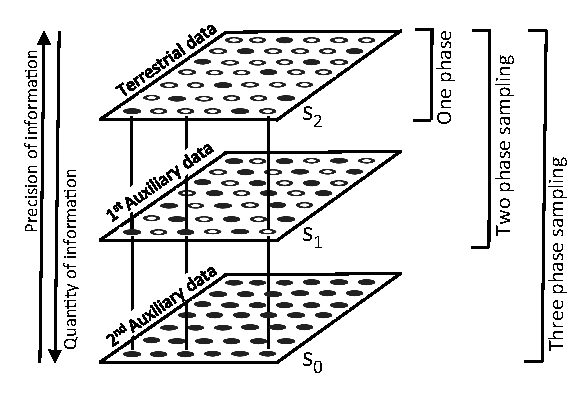
\includegraphics{Grafiken/Jstat_article/phases_graphic(new).eps}}%
		\caption{} \label{fig:concmphase_and_sae_a}
		\end{subfigure}
	\begin{subfigure}[t]{0.5\textwidth}
		\centering
	 \resizebox{0.58\hsize}{!}{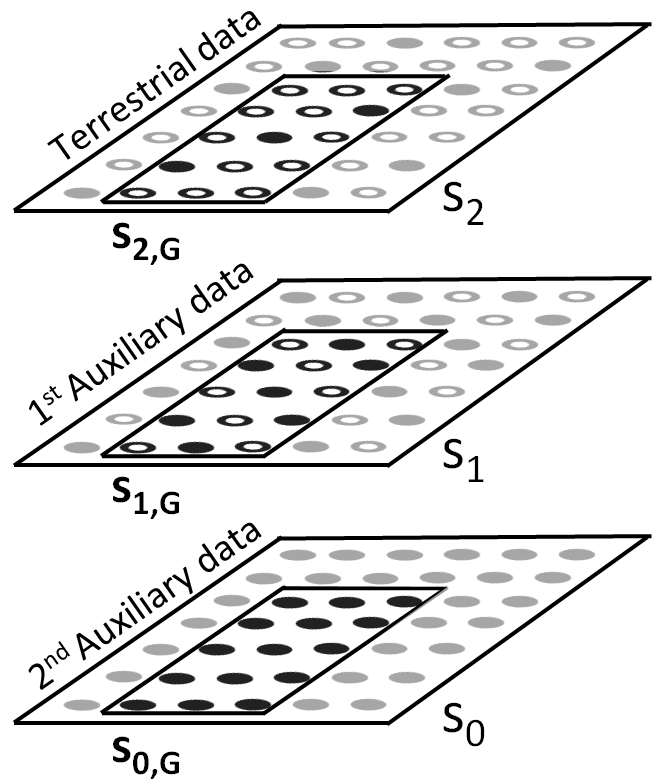
\includegraphics{Grafiken/Jstat_article/sae_graphic.PNG}}%
		\caption{} \label{fig:concmphase_and_sae_b}
	\end{subfigure}
\caption{(a) Concept of multi-phase sampling. The square represents the forest area for which an inventory is being conducted. The points denote the sample locations $x$. Filled points indicate available information. (b) Illustration of the small area estimation problem.}
\label{fig:concmphase_and_sae}
\end{figure}

\subsection{Small area estimation}

Small area estimation does not necessarily refer to small spatial areas but rather to areas that contain little or no terrestrial sample. To formulate this mathematically, we want to make an estimate for a subregion $G$ of the entire inventory area $F$ (Fig. \ref{fig:concmphase_and_sae_b}). As the sample size in the small area, $n_{2,G}$, is usually too small to provide sufficient estimation precision, multi-phase estimation can be efficient. However, $n_{2,G}$ may also be too small to justify fitting a separate regression model just for that area because the estimates produce undesirably large confidence intervals. The idea is then to borrow strength from the entire terrestrial sample $s_2$ of $F$ to fit the model, and to apply this model to the small area. The potential bias of applying that model in $G$ is then corrected for by using the empirical model residuals derived from that small area. If there are no terrestrial plots in $G$ (i.e., $n_{2,G}=0$), one cannot correct for a potential model bias in $G$ and has to accept a potential bias in the estimator. These are called synthetic estimates and despite their potential bias, it is usually still possible to calculate their design-based variance.


\subsection{Design-based vs. model-dependent approach}
\label{sec:db_vs_md}

The subject of model selection gets a lot of attention in the field of forest inventory. This is why it is important to understand that the mathematical interpretation of how a model is used to produce estimates is fundamentally different between the design-based and model-dependent approach. In the model-dependent (also known as model-based) framework, the sample locations $x$ are fixed and the observation $Y(x)$ taken at location $x$ is assumed to be a random variable as the forest is assumed to be the realization of a stochastic process. Although the model does not need to be fit from a probability sample, i.e., the sample locations could arbitrarily be chosen, the model should adequately describe the underlying stochastic process in order to efficiently ensure unbiased results. In practice this means that special attention must be made to ensure that the variable selection is appropriate to avoid overfitting, important variables are not omitted and all model assumptions are reasonably met through empirical verification. If a model is misspecified then estimation based on inference from that model may not be reliable. In the model-dependent framework one thus has to trust the model. In contrast, the design-based approach, on which all \pkg{forestinventory} estimators are based, rests upon the randomization of the sample locations $x$. While the sample locations $x$ are independently and uniformly distributed in the forest, the forest itself and thus the values of the local density surface at any location $x \in F$ are fixed and not the result of a stochastic process. A selected observation $Y(x)$ still remains a random variable, but solely due to the random sample mechanism. A consequence of this approach is that the estimation properties of design-based regression estimators (e.g., unbiasedness) typically hold regardless of the model that is chosen. The philosophy of the design-based approach is thus to use prediction models to improve the efficiency of the estimators without having to rely on their correct specification, which makes them very attractive to be used in official statistics. They are therefore also referred to as model-assisted. It should be noted that the randomization of sample locations upon which design-based inference depends, is in practice often replaced by systematic grids to minimize travelling costs in the terrestrial survey. However, there is reasonable evidence that softening this assumption is acceptable for point and variance estimation as long as the grid does not interact with periodic features in the forest structure \citep{mandallaz2008}. The variance will in most cases be slightly overestimated and lead to wider, more conservative confidence intervals \citep{mandallaz2013a}.

%\newpage

\subsection{Package structure}
\label{sec:packstruc}

In the \pkg{forestinventory} package, estimators for two-phase and three-phase sampling are applied with the \code{twophase()} and \code{threephase()} functions. From these two overall function calls, various estimators for specific inventory scenarios under the chosen sampling design can be applied (Fig. \ref{fig:struct_package}). Choosing an estimator follows a tree-like structure which can serve the user as a guideline throughout this article as well as in future applications. The basic decision to make is whether an estimate and its variance should be computed for an entire inventory area (global estimators) or only for subregions of the entire inventory area (small area estimators). In the second case, the package offers three small area estimators that will in detail be described in the following sections. The estimators are available under exhaustive and non-exhaustive use of the auxiliary data. Additionally, the package can also calculate one-phase estimates solely based on terrestrial samples. All estimators are also available for cluster sampling, in which case a sample unit consists of multiple, spatially agglomerated samples. The following sections describe the mathematical details and the application of the multi-phase estimators implemented in the \proglang{R} package \pkg{forestinventory}. While \cite{mandallaz2008, mandallaz2013techa, mandallaz2013techb,mandallaz2015tech} provides an extensive derivation of all estimators, we will provide the mathematical formulas that are actually implemented in the package. We will also restrict discussion to simple sampling, while the formulas for cluster sampling are available in the technical reports \citep{mandallaz2016, mandallaz2013techa, mandallaz2013techb}. A special case under cluster sampling is described in Section \ref{sec:speccas_and_scen}.

\begin{figure}[htb]
\centering
\resizebox{1\hsize}{!}{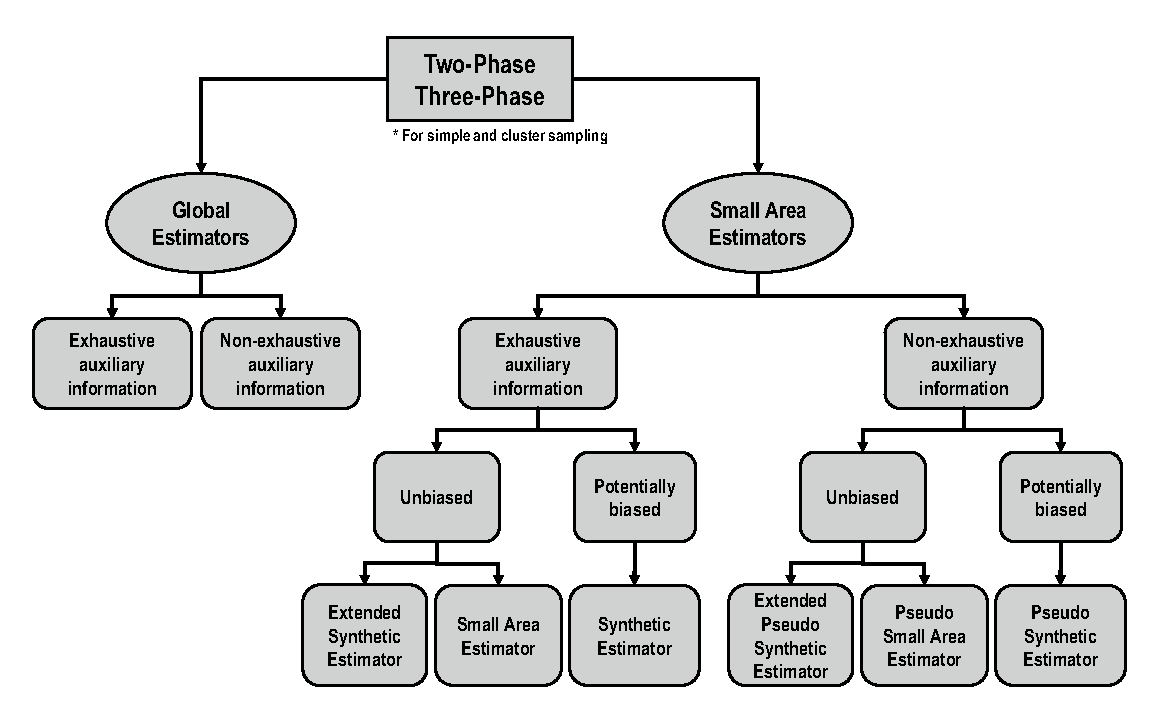
\includegraphics{Grafiken/Jstat_article/Package_structure_5.eps}}
\caption{Structure of the multi-phase estimators in the \proglang{R} package \pkg{forestinventory}.}
\label{fig:struct_package}
\end{figure}

\newpage


%------------------------------------------------------------------------------------------------%
% ---------------------------------- Estimators and their Application -------------------------- %

\section{Two-phase estimators and their application}
\label{sec:twophase_and_appl}


% ---------------------------------------------------------------------------- %
\subsection{Global estimators}
\label{sec:twophase_globest}

\subsubsection{Mathematical background}

The vector of regression coefficients of the OLS regression model is found by using the following solution to the sample-based normal equation:

\begin{equation}\label{normequ_simple}
  \hat{\pmb{\beta}}_{s_2}=\Big(\frac{1}{n_2}\sum_{x\in{s_2}}\pmb{Z}(x)\pmb{Z}^{\top}(x) \Big)^{-1} \Big(\frac{1}{n_2}\sum_{x\in{s_2}}Y(x)\pmb{Z}(x)\Big)
\end{equation}

The individual predictions can then be calculated as $\hat{Y}(x)=\pmb{Z}^{\top}(x)\hat{\pmb{\beta}}_{s_2}$ and the empirical model residuals, which are only available at all sample locations $x \in s_2$, are calculated as $\hat{R}(x)=Y(x)-\hat{Y}(x)$. Unless stated otherwise, \pkg{forestinventory} only uses internal models to calculate estimates. This means that the model fit, i.e., $\hat{\pmb{\beta}}_{s_2}$, is derived from the current inventory data that are passed to the \code{twophase()} and \code{threephase()} functions.  While virtually all inventorists fit their models using the current inventory data, sometimes there is reason to use formulas derived from external models where the sample used to train the model is assumed to be taken from an independent source \citep{massey2015a}. However, this usually occurs when using a model other than the OLS regression model and is beyond the scope of the package at this time.\par

The package provides the calculation of point estimates under exhaustive (EX) and non-exhaustive (NEX) use of the auxiliary information, which means to respectively apply $\hat{\pmb{\beta}}_{s_2}$ to $\bar{\pmb{Z}}$, i.e., the exact spatial mean of $\pmb{Z}(x)$, or to $\hat{\bar{\pmb{Z}}}$, i.e., an estimate of the spatial mean of $\pmb{Z}(x)$:


\begin{subequations}\label{eq:pointest_2p_reg}
\begin{align}
  \hat{Y}_{reg2p,EX} & =\bar{\pmb{Z}}^{\top}\hat{\pmb{\beta}}_{s_2} \label{eq:pointest_2p_reg_ex}\\
  \hat{Y}_{reg2p,NEX} & =\hat{\bar{\pmb{Z}}}^{\top}\hat{\pmb{\beta}}_{s_2} \label{eq:pointest_2p_reg_nex}
\end{align}
\end{subequations}

Note that for internal linear models the mean of the empirical residuals $\frac{1}{n_2}\sum_{x\in{s_2}}\hat{R}(x)$ is zero by construction (zero mean residual property) which is why it does not appear in the point estimate. More explanation about how to obain the auxiliary means is given in the next subsection.

The \pkg{forestinventory} package implements two kinds of variances for each of these point estimates: the g-weight formulation that accounts for the fact that our model is in fact internal, and the external variance formulation that assumes a true external regression model and thus neglects the uncertainty in the regression coefficients \citep{mandallaz2016}.

The g-weight formulation is

\begin{subequations}\label{eq:gw_var_2p_reg}
\begin{align}
  \hat{\var}(\hat{Y}_{reg2p,EX}) & :=\bar{\pmb{Z}}^{\top}\hat{\pmb{\Sigma}}_{\hat{\pmb{\beta}}_{s_2}}\bar{\pmb{Z}} \label{eq:gw_var_2p_reg_ex}\\
  \hat{\var}(\hat{Y}_{reg2p,NEX}) & :=
  \hat{\bar{\pmb{Z}}}^{\top}\hat{\pmb{\Sigma}}_{\hat{\pmb{\beta}}_{s_2}}\hat{\bar{\pmb{Z}}}
  + \hat{\pmb{\beta}}_{s_2}^{\top}\hat{\pmb{\Sigma}}_{\hat{\bar{\pmb{Z}}}}\hat{\pmb{\beta}}_{s_2} \label{eq:gw_var_2p_reg_nex}
\end{align}
\end{subequations}

where the g-weight variance-covariance matrix of $\hat{\pmb{\beta}}_{s_2}$ is calculated as

\begin{equation}\label{eq:estvarmatrix}
  \hat{\pmb{\Sigma}}_{\hat{\pmb{\beta}}_{s_2}}:=\Big(\frac{1}{n_2}\sum_{x\in{s_2}}\pmb{Z}(x)\pmb{Z}^{\top}(x) \Big)^{-1}
  \Big(\frac{1}{n_2^2}\sum_{x\in{s_2}}\hat{R}^2(x)\pmb{Z}(x)\pmb{Z}^{\top}(x)\Big)
  \Big(\frac{1}{n_2}\sum_{x\in{s_2}}\pmb{Z}(x)\pmb{Z}^{\top}(x) \Big)^{-1}
\end{equation}

and the uncertainty caused by using the $s_1$ sample to estimate $\bar{\pmb{Z}}$ by $\hat{\bar{\pmb{Z}}}$ is accounted for by the variance-covariance matrix of the auxiliary vector $\hat{\bar{\pmb{Z}}}$
\begin{equation}\label{estvarcovaux}
\hat{\Sigma}_{\hat{\bar{\pmb{Z}}}}=
\frac{1}{n_{1}(n_{1}-1)}\sum_{x\in{s_{1}}}
(\pmb{Z}(x)-\hat{\bar{\pmb{Z}}})(\pmb{Z}(x)-\hat{\bar{\pmb{Z}}})^{\top}
\end{equation}

The external variance formulation for linear regression models is

\begin{subequations}\label{eq:varexternal_2p_reg}
\begin{align}
  \hat{\var}_{ext}(\hat{Y}_{reg2p,EX}) & = \frac{1}{n_2}\hat{\var}_{s_2}(\hat{R}(x)) \label{eq:varexternal_2p_reg_ex} \\
  \hat{\var}_{ext}(\hat{Y}_{reg2p,NEX}) & = \frac{1}{n_1}\hat{\var}_{s_1}(\hat{Y}(x)) + \frac{1}{n_2}\hat{\var}_{s_2}(\hat{R}(x)) \nonumber  \label{eq:varexternal_2p_reg_nex}
\end{align}
\end{subequations}
where $\hat{\var}_{s_2}$ and $\hat{\var}_{s_1}$ indicate taking the sample variance over $s_2$ and $s_1$ respectively.

Note that when applied to internal linear regression models, the external variance is asymptotically unbiased and usually slightly smaller than the g-weight variance, where the uncertainty of the regression coefficients is accounted for by the variance-covariance matrix (Eq. \ref{eq:estvarmatrix}).  The external variances are provided in the package \pkg{forestinventory} in case the user wants to compare linear models to another model type where no g-weight formulation is possible, as is the case with non-parametric models like kNN.

\subsubsection{Calculation of explanatory variables}

We will now draw our attention to the calculation of the explanatory variables from the auxiliary data for both the non-exhaustive and exhaustive cases. Fig. \ref{fig:exh_nexh_and_boundweights_b} depicts how the non-exhaustive case often looks like in practice: a regular terrestrial grid $s_2$ is given by a terrestrial inventory (the points surrounded by dotted circles) and densified to a larger sample $s_1$ (the points). For every point $x$, each explanatory variable in the vector $\pmb{Z}(x)=(z(x)_1, z(x)_2,...,z(x)_p)^{\top}$ is calculated using a defined spatial extent of auxiliary information around that point called the support (the dark green square tiles). We emphasize that the value of the explanatory variables for $\pmb{Z}(x)$ are associated with the sample point whereas the support is the spatial extent of the auxiliary information used to calculate those values. So far this is in perfect agreement with the presented theory of the non-exhaustive estimator, except for using regular grids rather than randomly placed sample points. The \pkg{forestinventory} package calculates the empirical mean of $\pmb{Z}(x)$ automatically from the input data frame using $\hat{\bar{\pmb{Z}}}=\frac{1}{n_{1}}\sum_{x\in{s_{1}}}\pmb{Z}(x)$.\par

The exhaustive case requires a closer look. In the infinite population approach, $\pmb{Z}(x)$ refers to the sample point $x$ and not the area around it. Deriving the exact spatial mean, $\bar{\pmb{Z}}=\frac{1}{\lambda(F)}\int_{F} \pmb{Z}(x)dx= (\frac{1}{\lambda(F)}\int_{F} z_1(x)dx, ..., \frac{1}{\lambda(F)}\int_{F} z_p(x)dx)^{\top}$, implies that we need to calculate the spatial mean of each component of $\pmb{Z}(x)$ using all possible points in $F$. This is much like the situation we had with calculating the mean of the local density surface for $Y(x)$ in that we need to find the mean of $\pmb{Z}(x)$ over an infinite number of sample points (i.e., $n_1=\infty$). Although it is practically infeasible to assess $\pmb{Z}(x)$ for every $x$, there are few cases where the exact mean can in fact be precisely calculated. The first case is when the explanatory variables are provided by polygon layers (e.g., map of development stages). In this case, one can calculate the exact mean as the area-weighted average of each categorical variable. The second case is when the exact mean can be calculated in one step, e.g., taking the mean of all height pixels of a raster canopy height model will perfectly equal the mean calculated by the use of an infinite number of supports \citep{mandallaz2013b}. However, for most types of explanatory variables we will try to get an approximation of $\bar{\pmb{Z}}$ that is only negligibly different. \par

One implementation to approximate the exact mean $\bar{\pmb{Z}}$ is shown in Fig. \ref{fig:exh_nexh_and_boundweights_a}, where the spatial arrangement of the supports (the dark green tiles) are tessellated to form a perfect partition over the inventory area in order for all of the wall-to-wall auxiliary information to be exploited. Is has to be noted that this setup would allow for a perfect calculation of the exact mean $\bar{\pmb{Z}}$ in the finite population approach, i.e., deriving $\pmb{Z}(x)$ for the finite population of supports that are considered the sampling units. While in the infinite population approach this implementation probably does not produce the true exact mean $\bar{\pmb{Z}}$, $n_1$ is still expected to be reasonably large for the difference to be considered negligible as long as the size of the supports are not unreasonably large. However, the perfect tessellation implementation can also impose drawbacks. One is that a perfect tessellation by the supports strongly depends on the distance between the sample locations of $s_1$ and the support size. Since in practice the support size should ideally be chosen to achieve a best possible explanatory power of the regression model (thus minimizing the residual variation) a perfect tessellation might often not be feasible. In the infinite population frame, the supports are allowed to overlap if this seems necessary to acquire a sufficiently large sample $n_1$ to get a negligibly close approximation of $\bar{\pmb{Z}}$. With this respect, the infinite population approach provides more flexibility than the finite approach.

\begin{figure}[htb]
	\begin{subfigure}[t]{0.5\textwidth}
		\centering
    \resizebox{0.8\hsize}{!}{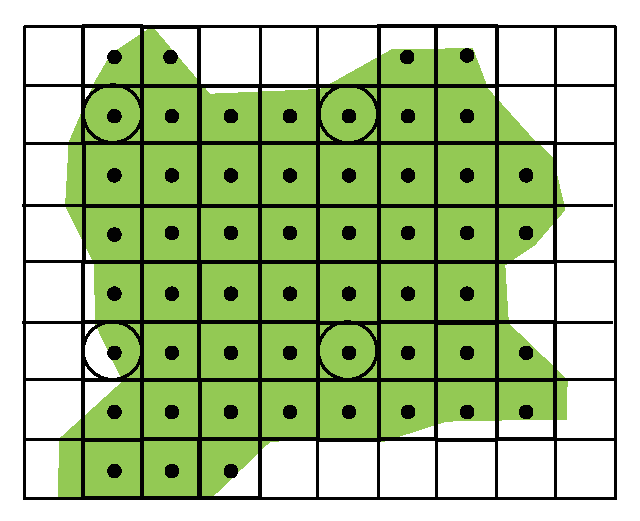
\includegraphics{Grafiken/Jstat_article/boundaryweight_graphic(left).eps}}%
		\caption{} \label{fig:exh_nexh_and_boundweights_a}
		\end{subfigure}
	\begin{subfigure}[t]{0.5\textwidth}
		\centering
   \resizebox{0.8\hsize}{!}{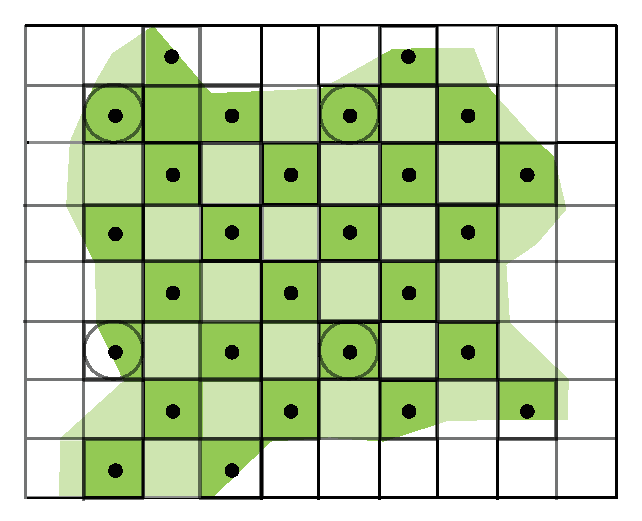
\includegraphics{Grafiken/Jstat_article/boundaryweight_graphic(right).eps}}%
		\caption{} \label{fig:exh_nexh_and_boundweights_b}
	\end{subfigure}
\caption{Concept of (a) exhaustive and (b) non-exhaustive calculation of explanatory variables including boundary adjustment at the support level. Auxiliary data are in both cases available over the entire inventory area marked by the large rectangle. A vector of explanatory variables $\pmb{Z}(x)$ is calculated within the supports (small squares)  at each sample location $x$ (points) that falls into the forest area (green underlying polygon).}
\label{fig:exh_nexh_bw}
\end{figure}

\subsubsection{Boundary adjustment}

An extension to the so-far published estimators by Mandallaz is the consideration of a boundary adjustment. In forest inventories, the sample is often restricted to those sample locations located within the forest area. In case a consistent forest definition can be applied to both the $s_2$ and $s_1$ sample (e.g., by a polygon forest mask layer), it might be desired to restrict the calculation of the explanatory variables to the forest area within the given support (see Fig. \ref{fig:exh_nexh_bw}). This method was suggested in \citet{mandallaz2013b} and led to an improvement in estimation precision. In order to ensure an unbiased calculation of either $\hat{\bar{\pmb{Z}}}$ or $\bar{\pmb{Z}}$, the respective means have then to be calculated as the weighted mean (Eq. \ref{eq:wmeanZ}) where the weight $w(x)$ is equal to the percentage of forested area within the support of sample location $x$.

\begin{equation}\label{eq:wmeanZ}
  \hat{\bar{\pmb{Z}}}=\frac{\sum_{x\in{s_1}}w(x)\pmb{Z}(x)}{\sum_{x\in{s_1}}w(x)}
\end{equation}

% --------------------------- %
\subsubsection{Application}

To demonstrate the use of the global two-phase estimators, we will use the \code{grisons} data set that comes with installing the package from the CRAN repository. The data set contains data from a simple (i.e., non-cluster) two-phase forest inventory conducted in 2007 that was used in \citet{mandallaz2013b} as a case study. The $s_1$ sample is comprised of 306 sample locations arranged on a systematic grid containing auxiliary information in the form of airborne laserscanning (LiDAR) canopy height metrics (\code{mean}, \code{stddev}, \code{max}, \code{q75}). For a systematic subsample of 67 ($s_2$ sample), terrestrial information of the timber volume per hectare (\code{tvol}) on the sample plot level is provided from a terrestrial survey. We can load \pkg{forestinventory} and examine the \code{grisons} data set in the \proglang{R} environment as follows:

\begin{small}
\begin{Schunk}
\begin{Sinput}
R> library("forestinventory")
R> data("grisons", package = "forestinventory")
R> head(grisons)
\end{Sinput}
\end{Schunk}
\end{small}

\begin{small}
\begin{Schunk}
\begin{Soutput}
   phase_id_2p boundary_weights  mean stddev   max   q75 smallarea   tvol
1            2             1.00  9.30  11.84 40.87 21.14         C 107.80
2            1             1.00 12.16  11.35 39.80 21.54         A     NA
3            2             1.00  5.25   5.74 23.82  9.53         D  63.77
4            1             1.00  7.53   9.33 34.10 13.02         A     NA
5            1             0.67  6.11   5.87 23.33 10.55         B     NA
6            1             1.00 12.15  10.16 33.76 20.97         C     NA
7            2             1.00  6.38   4.72 17.96 10.14         D 154.10
8            1             1.00  1.25   3.79 22.72  0.00         B     NA
9            1             1.00 21.56   7.49 32.66 27.81         A     NA
10           2             1.00 13.55   7.20 36.14 18.59         A 256.15
\end{Soutput}
\end{Schunk}
\end{small}

Estimates can be made using the \code{onephase()}, \code{twophase()} or \code{threephase()} functions. The data frame inputted to these functions must have the structure where each row corresponds to a unique sample location and the columns specify the attributes associated to that respective sample location. Attributes that are missing, e.g., because they are associated with sample locations that were not selected in the subsample for the subsequent phase, should be designated as \code{NA} and the phase membership is encoded as numeric.

For global two-phase estimation, we have to specify

\begin{itemize}
  \itemsep0em
  \item the regression model (\code{formula}) as specified in the \code{lm}()-function \citep{R}.
  \item the inputted \code{data.frame} containing the inventory information (\code{data}).
  \item the \code{list}-object \code{phase\_id} containing: the \code{phase.col} argument identifying the name of the column specifying membership to $s_1$ or $s_2$, and the \code{terrgrid.id} argument specifying which numeric value indicates $s_2$ membership in that column. Note that \pkg{forestinventory} implicitly assumes that all rows not indcated as $s_2$ belong to the $s_1$ phase.
  \item the name of the column containing the weights $w(x)$ of the boundary adjustments (optional).
\end{itemize}

The non-exhaustive estimator with boundary weight adjustment can thus be applied as follows:

\begin{small}
\begin{Schunk}
\begin{Sinput}
R> reg2p_nex <- twophase(formula = tvol ~ mean + stddev + max + q75, data = grisons, 
+    phase_id = list(phase.col = "phase_id_2p", terrgrid.id = 2),
+    boundary_weights = "boundary_weights")
\end{Sinput}
\end{Schunk}
\end{small}

The \code{twophase()} function creates an \code{S3} object of class \code{"twophase"} with subclass \code{"global"}. A readable summary of the estimation results can be obtained by passing this object to the \code{summary()} function, which automatically interprets what type of estimator was used and returns pertinent information such as the regression model formula, the point estimate (\code{estimate}), the g-weight and external variance (\code{g\_variance} and \code{ext\_variance}) as well as the sample sizes and the model R$^2$:

\begin{small}
\begin{Schunk}
\begin{Sinput}
R> summary(reg2p_nex)
\end{Sinput}
\begin{Soutput}
Two-Phase global estimation
 
Call: 
twophase(formula = tvol ~ mean + stddev + max + q75, data = grisons, 
    phase_id = list(phase.col = "phase_id_2p", terrgrid.id = 2), 
    boundary_weights = "boundary_weights")

Method used:
Non-exhaustive global estimator
 
Regression Model:
tvol ~ mean + stddev + max + q75

Estimation results:
 estimate ext_variance g_variance  n1 n2 r.squared
 383.5354      279.954   271.5057 306 67 0.6428771

'boundary_weight'- option was used to calculate weighted means of auxiliary variables
\end{Soutput}
\end{Schunk}
\end{small}

% \begin{Schunk}
% \begin{Sinput}
% Two-Phase global estimation
%  
% Call: 
% twophase(formula = tvol ~ mean + stddev + max + q75, data = grisons, 
%     phase_id = list(phase.col = "phase_id_2p", terrgrid.id = 2), 
%     boundary_weights = "boundary_weights")
% 
% Method used:
% Non-exhaustive global estimator
%  
% Regression Model:
% tvol ~ mean + stddev + max + q75
% 
% Estimation results:
%  estimate ext_variance g_variance  n1 n2 r.squared
%  383.5354      279.954   271.5057 306 67 0.6428771
% 
% 'boundary_weight'- option was used to calculate weighted means of auxiliary variables
% \end{Sinput}
% \end{Schunk}

For practical use, one should normally always prefer the g-weight variance over the external variance. This is because when we use internal models, the regression coefficients actually depend on the terrestrial sample realized by the sampling design. In contrast to the external variance, the g-weight variance accounts for this sampling variability which results in more reliable point and variance estimates and also enjoys better statistical calibration properties (g-weights). The external and g-weight variances are asymptotically equivalent but the external variance is really only included here in case the user wants to compare to another estimator where no g-weight variance exists.

The exhaustive estimator can be applied by additionally passing a vector containing the exact means of the explanatory variables, i.e., $\bar{\pmb{Z}}$, to the optional argument \code{exhaustive}. This vector must be calculated beforehand in such a way that any desired boundary adjustment has already been applied. Note that the vector input to \code{exhaustive} must be in the same order that the \code{lm()}-function processes a \code{formula} object including the intercept term whose exact mean will always be 1. Particular caution must be taken if categorical variables are present because the \code{lm()}-function, which is internally used to set up the design-matrix, automatically creates dummy variables with one of the categories used as a reference. Using our \code{grisons} example, the correct order can always be extracted by the following \proglang{R}-code:


\begin{small}
\begin{Schunk}
\begin{Sinput}
R> colnames(lm(formula = tvol ~ mean + stddev + max + q75, data = grisons, 
+    x = TRUE)$x)
\end{Sinput}
\end{Schunk}
\end{small}

The exhaustive estimator can be applied after defining the vector of exact means $\bar{\pmb{Z}}$ taken from \citet{mandallaz2013b}, denoted as \code{true.means.Z}:

\begin{small}
\begin{Schunk}
\begin{Sinput}
R> true.means.Z <- c(1, 11.39, 8.84, 32.68, 18.03)
R> reg2p_ex <- twophase(formula = tvol ~ mean + stddev + max + q75,
+    data = grisons,
+    phase_id = list(phase.col = "phase_id_2p", terrgrid.id = 2),
+    exhaustive = true.means.Z)
\end{Sinput}
\end{Schunk}
\end{small}

An alternative way to look at the estimation results without using the \code{summary()} is to query \code{reg2p\_ex} directly:
\begin{small}
\begin{Schunk}
\begin{Sinput}
R> reg2p_ex$estimation
\end{Sinput}
\begin{Soutput}
  estimate ext_variance g_variance  n1 n2 r.squared
1 376.7426     202.5602   187.2787 Inf 67 0.6428771
\end{Soutput}
\end{Schunk}
\end{small}
Note that both variances of the exhaustive estimation are smaller than those of the non-exhaustive estimation. This is essentially because we eliminated one component of uncertainty by substituting the estimated means of the explanatory variables $\hat{\bar{\pmb{Z}}}$ by their exact means $\bar{\pmb{Z}}$.


%--------------------------------------------------------------------------------------------------%
% ################################################################################################ %
%--------------------------------------------------------------------------------------------------%

\subsection{Small area estimators}
\label{sec:twophase_sae}

\subsubsection{Mathematical background}

The \pkg{forestinventory} package provides three types of small area estimators each of which has an exhaustive and non-exhaustive form. We will use a different nomenclature for the non-exhaustive case in small area estimation since much of the existing literature shows preference for the label pseudo to indicate that the mean of the explanatory variables within the small area was based on a finite sample. The main idea for all these small area estimators is to calculate the regression coefficient vector $\hat{\pmb{\beta}}_{s_2}$ and its variance-covariance matrix $\hat{\pmb{\Sigma}}_{\hat{\pmb{\beta}}_{s_2}}$ on the entire $s_2$ sample according to Eq. \ref{normequ_simple} and \ref{eq:estvarmatrix}, and subsequently use that to make predictions for sample locations restricted to small area $G$.\par

%----------------------------------------------- %
% \textbf{Small and Pseudo Small Area Estimator}\par

We first introduce the small area estimator (SMALL), which uses exhaustively computed explanatory variables, and its non-exhaustive version, the pseudo small area estimator (PSMALL). 

\begin{subequations}\label{eq:pest_2p_small_psmall}
\begin{align}
  \hat{Y}_{G,SMALL,2p} & =\bar{\pmb{Z}}_G^{\top}\hat{\pmb{\beta}}_{s_2} + \frac{1}{n_{2,G}}\hat{R}(x)  \label{eq:pointest_2p_small} \\
  \hat{Y}_{G,PSMALL,2p} & =\hat{\bar{\pmb{Z}}}_G^{\top}\hat{\pmb{\beta}}_{s_2} + \frac{1}{n_{2,G}}\hat{R}(x) \label{eq:pepsmall}
\end{align}
\end{subequations}

In the equations for the point estimates (Eq. \ref{eq:pointest_2p_small} and \ref{eq:pepsmall}), we see that the globally derived regression coefficients are applied to the exhaustively or non-exhaustively calculated means of the explanatory variables ($\bar{\pmb{Z}}_G$, $\hat{\bar{\pmb{Z}}}_G$) which are now only based on the first-phase sample $s_{1,G}$ located within small area $G$. A potential bias of the regression model predictions in the small area $G$, due to fitting the regression model with data also outside of $G$, is then corrected by adding the mean of the empirical model residuals in $G$. This is called the bias or residual correction term.

The package provides the g-weight variance for SMALL and PSMALL respectively (Eq. \ref{eq:var_2p_reg_small}, \ref{eq:var_2p_reg_psmall}) as well as the  external variance (Eq. \ref{eq:varext_2p_reg_small}, \ref{eq:varext_2p_reg_psmall}). Again note that all components are restricted to those available at the sample locations in the small area ($s_{1,G}$ and $s_{2,G}$), with exception of the regression coefficient components $\hat{\pmb{\beta}}_{s_2}$ and $\hat{\pmb{\Sigma}}_{\hat{\pmb{\beta}}_{s_2}}$.


\begin{subequations}\label{eq:var_2p_small_psmall}
\begin{align}
  \hat{\var}(\hat{Y}_{G,SMALL,2p}) & := \bar{\pmb{Z}}_G^{\top}\hat{\pmb{\Sigma}}_{\hat{\pmb{\beta}}_{s_2}}\bar{\pmb{Z}}_G
    + \frac{1}{n_{2,G}}\hat{\var}_{s_{2,G}}(\hat{R}(x))  \label{eq:var_2p_reg_small} \\
  \hat{\var}(\hat{Y}_{G,PSMALL,2p}) & := \hat{\bar{\pmb{Z}}}_G^{\top}\hat{\pmb{\Sigma}}_{\hat{\pmb{\beta}}_{s_2}}\hat{\bar{\pmb{Z}}}_G
  + \hat{\pmb{\beta}}_{s_2}^{\top}\hat{\Sigma}_{\hat{\bar{\pmb{Z}}}_G}\hat{\pmb{\beta}}_{s_2}
  + \frac{1}{n_{2,G}}\hat{\var}_{s_{2,G}}(\hat{R}(x))  \label{eq:var_2p_reg_psmall}
\end{align}
\end{subequations}

\begin{subequations}\label{eq:varext_2p_small_psmall}
\begin{align}
  \hat{\var}_{ext}(\hat{Y}_{G,SMALL,2p}) & := \frac{1}{n_{2,G}}\hat{\var}_{s_{2,G}}(\hat{R}(x))  \label{eq:varext_2p_reg_small} \\
  \hat{\var}_{ext}(\hat{Y}_{G,PSMALL,2p}) & := \frac{1}{n_{1,G}}\hat{\var}_{s_{2,G}}(Y(x)) + \Big(1-\frac{n_{2,G}}{n_{1,G}}\Big)\frac{1}{n_{2,G}}\hat{\var}_{s_{2,G}}(\hat{R}(x)) \label{eq:varext_2p_reg_psmall}
\end{align}
\end{subequations}
where $\hat{\var}_{s_{2,G}}$ indicates taking the sample variance over $s_{2,G}$. If boundary adjustment is applied, the simple mean of the explanatory variable vector over the small area $\hat{\bar{\pmb{Z}}}_G=\frac{1}{n_{1,G}}\sum_{x \in s_{1,G}}\pmb{Z}(x)$ is replaced by its weighted version $\hat{\bar{\pmb{Z}}}_G=\frac{\sum_{x\in{s_{1,G}}}w(x)\pmb{Z}(x)}{\sum_{x\in{s_{1,G}}}w(x)}$, and likewise for exhaustively used auxiliary information.



%------------------------------------------------------------- %
% \textbf{Synthetic and Pseudo Synthetic Estimator}\par

The synthetic estimator (SYNTH) and pseudo synthetic estimator (PSYNTH) are commonly applied when no terrestrial sample is available within the small area $G$ (i.e., $n_{2,G}=0$). In this case, the point estimates (Eq. \ref{eq:pointest_2p_reg_synth} and \ref{eq:pointest_2p_reg_psynth}) are based only on the predictions generated by applying the globally derived regression model to the auxiliary vectors $\bar{\pmb{Z}}_G$ and $\hat{\bar{\pmb{Z}}}_G$ respectively. However, the bias correction using the observed residuals $\hat{R}(x)$ is not applied as was the case in the small and pseudo small area estimator (Eq. \ref{eq:pointest_2p_small} and \ref{eq:pepsmall}). Thus, the (pseudo) synthetic estimator has a potentially unobservable design-based bias. Also note that the residual variation can no longer be considered in the g-weight variance (Eq. \ref{eq:var_2p_reg_synth} and \ref{eq:var_2p_reg_psynth}). Therefore, the synthetic estimators will usually have a smaller variance than estimators incorporating the regression model uncertainties, but at the cost of a potential bias. Due to the absence of available residuals in $G$, there is also no external variance form for the synthetic and pseudo synthetic estimator.

% Left out for simplicity reasons in article, maybe include in Diss:
% However, this assumption is unlikely to be fullfilled in practice resulting in a potentially unobservable design-based bias equal to $-\frac{1}{\lambda(G)}\int_G R(x)$. 

\begin{subequations}\label{eq:pest_2p_synth_psynth}
\begin{align}
  \hat{Y}_{G,SYNTH,2p} & =\bar{\pmb{Z}}_G^{\top}\hat{\pmb{\beta}}_{s_2} \label{eq:pointest_2p_reg_synth} \\
  \hat{Y}_{G,PSYNTH,2p} & =\hat{\bar{\pmb{Z}}}_G^{\top}\hat{\pmb{\beta}}_{s_2} \label{eq:pointest_2p_reg_psynth} \\
  \hat{\var}(\hat{Y}_{G,SYNTH,2p}) & = \bar{\pmb{Z}}_G^{\top}\hat{\pmb{\Sigma}}_{\hat{\pmb{\beta}}_{s_2}}\bar{\pmb{Z}}_G \label{eq:var_2p_reg_synth} \\
  \hat{\var}(\hat{Y}_{G,PSYNTH,2p}) & = \hat{\bar{\pmb{Z}}}_G^{\top}\hat{\pmb{\Sigma}}_{\hat{\pmb{\beta}}_{s_2}}\hat{\bar{\pmb{Z}}}_G
  + \hat{\pmb{\beta}}_{s_2}^{\top}\hat{\pmb{\Sigma}}_{\hat{\bar{\pmb{Z}}}_G}\hat{\pmb{\beta}}_{s_2}  \label{eq:var_2p_reg_psynth}
\end{align}
\end{subequations}

where the variance-covariance matrix of the auxiliary vector $\hat{\bar{\pmb{Z}}}_G$ is estimated by
\begin{equation}\label{estvarcovaux_G}
\hat{\Sigma}_{\hat{\bar{\pmb{Z}}}_{G}}=
\frac{1}{n_{1,G}(n_{1,G}-1)}\sum_{x\in{s_{1,G}}}
(\pmb{Z}(x)-\hat{\bar{\pmb{Z}}}_{G})(\pmb{Z}(x)-\hat{\bar{\pmb{Z}}}_{G})^{\top}
\end{equation}

%------------------------------------------------------------- %
% \textbf{Extended Synthetic and Extended Pseudo Synthetic Estimator}\par

The synthetic estimators, SYNTH and PSYNTH, have attractively compact formulas but come with the downside of potential bias in their point estimates which can make the variances seem deceptively optimistic. The SMALL and PSMALL estimators overcome this issue by using a bias correction term, i.e., $\frac{1}{n_{2,G}}\sum_{x \in s_{2,G}}\hat{R}(x)$. The motivation behind the extended synthetic and extended pseudo synthetic estimator (EXTSYNTH and EXTPSYNTH) is to use the same mathematically elegant formulas of the (pseudo) synthetic estimators while ensuring that the mean of the empirical prediction model residuals in the entire area $F$ and the small area $G$ are by construction both zero at the same time. This is accomplished by extending the vector of auxiliary information $\pmb{Z}(x)$ by a binary categorical indicator variable $I_G(x)$ which takes the value 1 if the sample location $x$ lies inside the target small area $G$ and is otherwise set to 0. Recalling that linear models fitted using OLS have zero mean residual property by construction also if categorical variables are used, this leads to unbiased point estimates. The new extended auxiliary vector thus becomes $\pmb{\mathbb{Z}}^{\top}(x)=(\pmb{Z}^{\top}(x),I^{\top}_G(x))$ and can be used to replace its non-extended counterpart $\pmb{Z}^{\top}(x)$ whereever it is used in Eq. \ref{eq:pest_2p_synth_psynth} and \ref{estvarcovaux_G}. Note that the package functions internally extend the data set by the indicator variable if the EXTSYNTH or EXTPSYNTH estimator is called.

Not every equation needs to be re-written here, but to give an example of the notational change, the regression coefficient under extended model approach becomes

\begin{equation}\label{ext_normequ_simple}
  \hat{\pmb{\theta}}_{s_2}=\Big(\frac{1}{n_2}\sum_{x\in{s_2}}\pmb{\mathbb{Z}}(x)\pmb{\mathbb{Z}}^{\top}(x) \Big)^{-1} \Big(\frac{1}{n_2}\sum_{x\in{s_2}}Y(x)\pmb{\mathbb{Z}}(x)\Big)
\end{equation}

The point estimates and their g-weight variances can then be re-written as

\begin{subequations}\label{eq:pest_2p_extsynth_extpsynth}
\begin{align}
\hat{Y}_{G,EXTSYNTH,2p} & = \bar{\pmb{\mathbb{Z}}}^{\top}_{G}\hat{\pmb{\theta}}_{s_2} \label{eq:pointest_2p_extsynth} \\
\hat{Y}_{G,EXTPSYNTH,2p} & =\hat{\bar{\pmb{\mathbb{Z}}}}_{G}^{\top}\hat{\pmb{\theta}}_{s_2} \label{eq:pointest_2p_extsynth} \\
\hat{\var}(\hat{Y}_{G,EXTSYNTH,2p}) & = \bar{\pmb{\mathbb{Z}}}^{\top}_{G}\hat{\pmb{\Sigma}}_{\hat{\pmb{\theta}}_{s_2}}\bar{\pmb{\mathbb{Z}}}_{G} \label{eq:var_2p_extsynth} \\
\hat{\var}(\hat{Y}_{G,EXTPSYNTH,2p})& =
\hat{\bar{\pmb{\mathbb{Z}}}}_{G}^{\top}\hat{\pmb{\Sigma}}_{\hat{\pmb{\theta}}_{s_2}}
\hat{\bar{\pmb{\mathbb{Z}}}}_{G}
+ \hat{\pmb{\theta}}^{\top}_{s_2}\hat{\pmb{\Sigma}}_{\hat{\bar{\pmb{\mathbb{Z}}}}_{G}}\hat{\pmb{\theta}}_{s_2} \label{eq:var_2p_extpsynth}
\end{align}
\end{subequations}

While the formulas look similar to the synthetic estimators, note that a decomposition of $\hat{\pmb{\theta}}_{s_2}$ reveals that the residual correction term is now included in the regression coefficient $\hat{\pmb{\theta}}_{s_2}$ \citep{mandallaz2016} and thus the estimates are asymptotically design-unbiased.

The package also provides the external variance for both the extended synthetic and extended pseudo synthetic estimator. Note that neither the extended model approach nor external variance estimates are possible in the absence of terrestrial samples and thus model residuals in $G$, which is precisely when one must rely on the (pseudo) synthetic estimates. The external variance forms of EXTSYNTH and EXTPSYNTH are

\begin{subequations}\label{eq:ext_varexternal_2p_extsynth}
\begin{align}
  \hat{\var}_{ext}(\hat{Y}_{G,EXTSYNTH,2p}) & = \frac{1}{n_{2,G}}\hat{\var}_{s_{2,G}}(\hat{\mathbb{R}}(x)) \label{eq:ext_varexternal_2p_extsynth} \\
  \hat{\var}_{ext}(\hat{Y}_{G,EXTPSYNTH,2p}) & = \frac{1}{n_{1,G}}\hat{\var}_{s_{2,G}}(Y(x)) + \Big(1-\frac{n_{2,G}}{n_{1,G}}\Big)\frac{1}{n_{2,G}}\hat{\var}_{s_{2_G}}(\hat{\mathbb{R}}(x)) \label{eq:ext_varexternal_2p_extpsynth}
\end{align}
\end{subequations}
where $\hat{\mathbb{R}}(x)$ are the empirical residuals under the extended auxiliary vector.

To summarize, the synthetic estimators SYNTH and PSYNTH can be applied whether terrestrial inventory sample is found in the small area or not, but has a deceptively small g-weight variance due to its potential bias.  When terrestrial sample is observed in the small area, we can produce (asymptotically) design-unbiased estimates and variances using either SMALL or PSMALL which remove this bias explicitly with a mean residual term, or more elegantly with EXTSYNTH or EXTPSYNTH which simply use the same synthetic formulas while including an indicator variable for the small area in the model formula to remove the bias by construction in OLS.


%------------------------------------------------------------- %
\subsubsection{Application}

Small area estimates in the \pkg{forestinventory} package can be applied by specifying the optional argument \code{small\_area}. The input data set has to include an additional column of class \code{factor} that describes the small area membership of the sample location represented by that row. The argument \code{small\_area} requires a \code{list}-object that comprises

\begin{itemize}
  \itemsep0em
  \item the name of the column specifiying the small area of each observation (\code{sa.col}).
  \item a vector specifying the small area(s) for which estimations are desired (\code{areas}).
  \item the argument \code{unbiased} that controls which of the three available estimators is applied.
\end{itemize}

In order to apply the pseudo small area estimator (PSMALL) with boundary adjustment, we set \code{unbiased=TRUE} as well as the optional argument \code{psmall=TRUE}:
\begin{small}
\begin{Schunk}
\begin{Sinput}
R> psmall_2p <- twophase(formula = tvol ~ mean + stddev + max + q75, 
+    data = grisons, phase_id = list(phase.col = "phase_id_2p", terrgrid.id = 2),
+    small_area = list(sa.col = "smallarea", areas = c("A", "B"),
+    unbiased = TRUE), psmall = TRUE, boundary_weights = "boundary_weights")
\end{Sinput}
\end{Schunk}
\end{small}

\begin{small}
\begin{Schunk}
\begin{Sinput}
R> summary(psmall_2p)
\end{Sinput}
\begin{Soutput}
Two-phase small area estimation
 
Call: 
twophase(formula = tvol ~ mean + stddev + max + q75, data = grisons, 
    phase_id = list(phase.col = "phase_id_2p", terrgrid.id = 2), 
    small_area = list(sa.col = "smallarea", areas = c("A", "B"), 
        unbiased = TRUE), boundary_weights = "boundary_weights", 
    psmall = TRUE)

Method used:
Pseudo small area estimator
 
Regression Model:
tvol ~ mean + stddev + max + q75

Estimation results:
 area estimate ext_variance g_variance  n1 n2 n1G n2G r.squared
    A 393.9713     1009.034   1308.117 306 67  94  19 0.6428771
    B 419.6416     1214.035   1259.472 306 67  81  17 0.6428771

'boundary_weight'- option was used to calculate weighted means of auxiliary variables
\end{Soutput}
\end{Schunk}
\end{small}

The small area functions all return an \code{S3} object of class \code{"twophase"} with subclass \code{"smallarea"}. In addition to global estimation, the \code{estimation} object now comprises the estimates and variances for all small areas (column \code{area}). We can view the sample sizes by looking into the object itself
\begin{small}
\begin{Schunk}
\begin{Sinput}
R> psmall_2p$samplesizes
\end{Sinput}
\begin{Soutput}
$A
      n1G n2G  n1 n2
plots  94  19 306 67

$B
      n1G n2G  n1 n2
plots  81  17 306 67
\end{Soutput}
\end{Schunk}
\end{small}

The extended pseudo synthetic estimator (EXTPSYNTH) can be applied by setting \code{unbiased=TRUE} and leaving the optional argument \code{psmall} to its default value of \code{FALSE}:


\begin{small}
\begin{Schunk}
\begin{Sinput}
R> extpsynth_2p <- twophase(formula = tvol ~ mean + stddev + max + q75, 
+    data = grisons, phase_id = list(phase.col = "phase_id_2p", terrgrid.id = 2),
+    small_area = list(sa.col = "smallarea", areas = c("A", "B"),
+    unbiased = TRUE), boundary_weights = "boundary_weights")
R> extpsynth_2p$estimation
\end{Sinput}
\begin{Soutput}
  area estimate ext_variance g_variance  n1 n2 n1G n2G r.squared
1    A 391.9356     995.5602   1017.633 306 67  94  19 0.6526503
2    B 419.7231    1214.6053   1019.191 306 67  81  17 0.6428854
\end{Soutput}
\end{Schunk}
\end{small}

The \pkg{forestinventory} package automatically includes the indicator variable for the small area behind the scenes so there is no need for the user to implement it. Notice that the $R^2$s (\code{r.squared}) under the EXTPSYNTH estimator vary between the small areas, while they are identical under the PSMALL estimator. This is because under the EXTPSYNTH estimator, the regression model is recalculated for each small area estimation after adding the indicator variable for the respective small area in the globally derived design matrix. In case of the PSMALL estimator, the regression model stays the same for each small area estimation. Although the results of both estimators should always be close to each other, we recommend applying both estimators and compare the results afterwards in order to reveal unsuspected patterns in the data, particularly in the case of cluster sampling (see Section \ref{sec:speccas_and_scen}).\par

Setting the argument \code{unbiased=FALSE} applies the pseudo synthetic estimator to the selected small areas. Note that in the \code{grisons} data set, all small areas possess much more than the suggested minimum number of terrestrial observations (a rule of thumb is that $n_{2,G} \geq 6$) required to produce reliable design-unbiased estimates. Hence, choosing to use PSYNTH is probably not desireable and is just applied here for demonstration purposes. In this case the residual correction will not be applied.


\begin{small}
\begin{Schunk}
\begin{Sinput}
R> psynth_2p <- twophase(formula = tvol ~ mean + stddev + max + q75, 
+    data = grisons, phase_id = list(phase.col = "phase_id_2p", terrgrid.id = 2),
+    small_area = list(sa.col = "smallarea", areas = c("A", "B"),
+    unbiased = FALSE), boundary_weights = "boundary_weights")
\end{Sinput}
\end{Schunk}
\end{small}

\begin{small}
\begin{Schunk}
\begin{Sinput}
R> psynth_2p$estimation
\end{Sinput}
\begin{Soutput}
  area estimate ext_variance g_variance  n1 n2 n1G n2G r.squared
1    A 421.8863           NA   546.8651 306 67  94  19 0.6428771
2    B 418.7399           NA   566.3361 306 67  81  17 0.6428771
\end{Soutput}
\end{Schunk}
\end{small}

We see here that the PSYNTH variances are almost only half the variances of the PSMALL and EXTPSYNTH estimator. However, PSMALL and EXTPSYNTH are design unbiased and their variances reflect the fact that they account for potential bias of the regression model predictions. The g-weight variance of PSYNTH completely neglects a potential bias and as a result risks severely overstating the estimation precision.\par

The exhaustive versions of the small area estimators (Eq. \ref{eq:pointest_2p_small}, \ref{eq:var_2p_reg_small}, \ref{eq:varext_2p_reg_small}, \ref{eq:pointest_2p_reg_synth}, \ref{eq:var_2p_reg_synth}) are specified via the optional argument \code{exhaustive}. Its application requires that we know the exact means of all explanatory variables within the small area(s) of interest. In contrast to the global estimators, the exact means have now to be delivered in the form of a \code{data.frame}, where each row corresponds to a small area, and each column specifies the exact mean of the respective explanatory variable. Note that likewise the case of global estimation, the order of the explanatory variables in the data frame has to match the order in which they appear in the design matrix defined by the \code{lm()}-function in \proglang{R}. In order to tell \proglang{R} which row describes which small area, the row names have to match the respective names of the small areas specified in the \code{areas} argument.

For the \code{grisons} data set, the exact means of the explanatory variables for the small areas used in \citet{mandallaz2013b} are thus defined by
\begin{small}
\begin{Schunk}
\begin{Sinput}
R> colnames(lm(formula = tvol ~ mean + stddev + max + q75, data = grisons, 
+    x = TRUE)$x)
\end{Sinput}
\end{Schunk}
\end{small}
\begin{small}
\begin{Schunk}
\begin{Sinput}
R> true.means.Z.G <- data.frame(Intercept = rep(1, 4),
+    mean = c(12.85, 12.21, 9.33, 10.45),
+    stddev = c(9.31, 9.47, 7.90, 8.36),
+    max = c(34.92, 35.36, 28.81, 30.22),
+    q75 = c(19.77, 19.16, 15.40, 16.91))
R> rownames(true.means.Z.G) <- c("A", "B", "C", "D")
\end{Sinput}
\end{Schunk}
\end{small}
\begin{small}
\begin{Schunk}
\begin{Sinput}
R> true.means.Z.G
\end{Sinput}
\begin{Soutput}
  Intercept  mean stddev   max   q75
A         1 12.85   9.31 34.92 19.77
B         1 12.21   9.47 35.36 19.16
C         1  9.33   7.90 28.81 15.40
D         1 10.45   8.36 30.22 16.91
\end{Soutput}
\end{Schunk}
\end{small}

The extended synthetic estimator (EXTSYNTH) can then be applied by
\begin{small}
\begin{Schunk}
\begin{Sinput}
R> extsynth_2p <- twophase(formula = tvol ~ mean + stddev + max + q75, 
+    data = grisons, phase_id = list(phase.col = "phase_id_2p", terrgrid.id = 2),
+    small_area = list(sa.col ="smallarea", areas = c("A", "B"),
+    unbiased = TRUE), exhaustive = true.means.Z.G)
\end{Sinput}
\end{Schunk}
\end{small}

\begin{small}
\begin{Schunk}
\begin{Sinput}
R> extsynth_2p$estimation
\end{Sinput}
\begin{Soutput}
  area estimate ext_variance g_variance  n1 n2 n1G n2G r.squared
1    A 372.6930     744.3658   696.5739 Inf 67 Inf  19 0.6526503
2    B 387.5116     693.8576   708.1105 Inf 67 Inf  17 0.6428854
\end{Soutput}
\end{Schunk}
\end{small}

Just as in the global case, we see that the variance has again been significantly decreased by substituting the exact auxiliary means and both first phase sample sizes are now infinity. Note that the function extracts the required exact means for small area \code{"A"} and \code{"B"} from the complete set of exact means defined in \code{true.means.Z.G}.

\newpage

\section{Three-phase estimators and their application}
\label{sec:threephase_and_appl}

% ---------------------------------------------------------------------------- %
% ---------------------------------------------------------------------------- %
\subsection{Global estimators}
\label{sec:glob_est_3p}


% ------------------------------------- %
\subsubsection{Mathematical background}


Solving the sample-based normal equations, the vector of regression coefficients $\hat{\pmb{\alpha}}_{s_2}$ for the reduced model, i.e., using the reduced set of explanatory variables $\pmb{Z}^{(0)}(x)$ available at $x \in s_0$, and likewise the vector of regression coefficients $\hat{\pmb{\beta}}_{s_2}$ for the full model, i.e., using the full set of explanatory variables $\pmb{Z}^{\top}(x)=(\pmb{Z}^{(0)\top}(x),\pmb{Z}^{(1)\top}(x))$ available only at a subset $x \in s_1 \subset s_0$, are derived as

\begin{subequations}\label{eq:normequ_3p}
\begin{align}
\hat{\pmb{\alpha}}_{s_2}&=\Big(\frac{1}{n_2}\sum_{x\in{s}_2}\pmb{Z}^{(0)}(x)\pmb{Z}^{(0)\top}(x)
\Big)^{-1}\frac{1}{n_2}\sum_{x\in{s}_2}Y(x)\pmb{Z}^{(0)}(x)  \label{eq:normequ_redmod} \\
\hat{\pmb{\beta}}_{s_2}&=\Big(\frac{1}{n_2}\sum_{x\in{s}_2}\pmb{Z}(x)\pmb{Z}^{\top}(x)
\Big)^{-1}\frac{1}{n_2}\sum_{x\in{s}_2}Y(x)\pmb{Z}(x) \label{eq:normequ_fullmod}
\end{align}
\end{subequations}

The package allows for the calculation of point estimates under exhaustive and non-exhaustive use of the auxiliary information in the $s_0$ phase. Fitting the model using $s_2$ (i.e., internally) ensures the zero mean residual property over $s_2$.

\begin{subequations}\label{eq:reg3p}
\begin{align}
\hat{Y}_{reg3p,EX}&=\frac{1}{\lambda(F)}\int_{F} \pmb{Z}^{(0)\top}(x)\hat{\pmb{\alpha}}_{s_2} + \frac{1}{n_1}\sum_{x\in s_1} (\pmb{Z}^{\top}(x)\hat{\pmb{\beta}}_{s_2}-\pmb{Z}^{(0)\top}(x)\hat{\pmb{\alpha}}_{s_2}) + \frac{1}{n_2}\sum_{x\in s_2}(Y(x)-\pmb{Z}^{\top}(x)\hat{\pmb{\beta}}_{s_2})
\nonumber \\&= (\bar{\pmb{Z}}^{(0)}_0-\hat{\bar{\pmb{Z}}}^{(0)}_1)^{\top}\hat{\pmb{\alpha}}_{s_2} +
\hat{\bar{\pmb{Z}}}^{\top}_1\hat{\pmb{\beta}}_{s_2} \label{eq:reg3p_ex} \\
\hat{Y}_{reg3p,NEX}&=\frac{1}{n_0}\sum_{x\in s_0} \pmb{Z}^{(0)\top}(x)\hat{\pmb{\alpha}}_{s_2} + \frac{1}{n_1}\sum_{x\in s_1} (\pmb{Z}^{\top}(x)\hat{\pmb{\beta}}_{s_2}-\pmb{Z}^{(0)\top}(x)\hat{\pmb{\alpha}}_{s_2}) + \frac{1}{n_2}\sum_{x\in s_2}(Y(x)-\pmb{Z}^{\top}(x)\hat{\pmb{\beta}}_{s_2})
\nonumber \\&=(\hat{\bar{\pmb{Z}}}^{(0)}_0-\hat{\bar{\pmb{Z}}}^{(0)}_1)^{\top}\hat{\pmb{\alpha}}_{s_2}  +
\hat{\bar{\pmb{Z}}}^{\top}_1\hat{\pmb{\beta}}_{s_2} \label{eq:reg3p_nex}
\end{align}
\end{subequations}

Intuitively, the three phase estimator is simply the mean of the predictions using the reduced model, corrected by the mean difference between the reduced model predictions and the more accurate full model predictions, corrected by the mean difference between the ground truth and the full model predictions. For the compact version of the formula in the non-exhaustive case, the estimated means of $\pmb{Z}^{(0)}(x)$ over both the $s_0$ and $s_1$ phase, as well as the estimated mean of $\pmb{Z}(x)$ over the $s_1$ phase are calculated according to Eq. \ref{meanvalues3pnex}. If the exact mean over $s_0$ is known, the estimated mean $\hat{\bar{\pmb{Z}}}^{(0)}_0$ can simply be replaced by the exact mean $\bar{\pmb{Z}}^{(0)}_0$. Note that in case of applied boundary adjustment (Section \ref{sec:twophase_and_appl}), the simple mean is again replaced by the weighted mean analogous to Eq. \ref{eq:wmeanZ}.

\begin{equation}\label{meanvalues3pnex}
\hat{\bar{\pmb{Z}}}^{(0)}_0=\frac{1}{n_0}\sum_{x\in{s_0}} \pmb{Z}^{(0)}(x), \quad \hat{\bar{\pmb{Z}}}^{(0)}_1=\frac{1}{n_1}\sum_{x\in{s}_1}\pmb{Z}^{(0)}(x) ,
\quad \hat{\bar{\pmb{Z}}}_1=\frac{1}{n_1}\sum_{x\in{s}_1}\pmb{Z}(x)
\end{equation}

The package again provides the g-weight and external variances. The g-weight variance formulation is

\begin{subequations}\label{eq:dbvar_reg3p}
\begin{align}
\hat{\var}(\hat{Y}_{reg3p,EX})& =\frac{n_2}{n_1}\bar{\pmb{Z}}^{(0)\top}\hat{\pmb{\Sigma}}_{\hat{\pmb{\alpha}}_{s_2}}
\bar{\pmb{Z}}^{(0)}+(1-\frac{n_2}{n_1})\hat{\bar{\pmb{Z}}}_1^{\top}\hat{\pmb{\Sigma}}_{\hat{\pmb{\beta}}_{s_2}}
\hat{\bar{\pmb{Z}}}_1 \label{eq:dbvar_reg3p_ex} \\
\hat{\var}(\hat{Y}_{reg3p,NEX})& =\hat{\pmb{\alpha}}_{s_2} ^{\top}\hat{\pmb{\Sigma}}_{\hat{\bar{\pmb{Z}}}^{(0)}_0}\hat{\pmb{\alpha}}_{s_2}
+\frac{n_2}{n_1}\hat{\bar{\pmb{Z}}}^{(0)\top}_0
\hat{\pmb{\Sigma}}_{\hat{\pmb{\alpha}}_{s_2}}\hat{\bar{\pmb{Z}}}^{(0)}_0 + (1-\frac{n_2}{n_1})\hat{\bar{\pmb{Z}}}^{\top}_1\hat{\pmb{\Sigma}}_{\hat{\pmb{\beta}}_{s_2}}\hat{\bar{\pmb{Z}}}_1 \label{eq:dbvar_reg3p_nex}
\end{align}
\end{subequations}

with the variance-covariance matrix of $\hat{\bar{\pmb{Z}}}^{(0)}_0$ and the variance-covariance matrices of the regression coefficients $\hat{\pmb{\alpha}}_{s_2}$ and $\hat{\pmb{\beta}}_{s_2}$:

\begin{subequations}\label{eq:covar3p}
\begin{align}
  \hat{\pmb{\Sigma}}_{\hat{\bar{\pmb{Z}}}^{(0)}_0}&=
  \frac{1}{n_{0}(n_{0}-1)}\sum_{x\in{s_{0}}}
  (\pmb{Z}^{(0)}(x)-\hat{\bar{\pmb{Z}}}^{(0)}_{0})(\pmb{Z}^{(0)}(x)-\hat{\bar{\pmb{Z}}}^{(0)}_{0})^{\top} \\
  \hat{\pmb{\Sigma}}_{\hat{\pmb{\alpha}}_{s_2}}&=\Big(\frac{1}{n_2}\sum_{x\in{s_2}}\pmb{Z}^{(0)}(x)\pmb{Z}^{(0)\top}(x) \Big)^{-1}
  \Big(\frac{1}{n_2^2}\sum_{x\in{s_2}}\hat{R}^{(0)2}(x)\pmb{Z}^{(0)}(x)\pmb{Z}^{(0)\top}(x)\Big)
  \Big(\frac{1}{n_2}\sum_{x\in{s_2}}\pmb{Z}^{(0)}(x)\pmb{Z}^{(0)\top}(x) \Big)^{-1} \label{eq:covar_alpha} \\
  \hat{\pmb{\Sigma}}_{\hat{\pmb{\beta}}_{s_2}}&=\Big(\frac{1}{n_2}\sum_{x\in{s_2}}\pmb{Z}(x)\pmb{Z}^{\top}(x) \Big)^{-1}
  \Big(\frac{1}{n_2^2}\sum_{x\in{s_2}}\hat{R}^2(x)\pmb{Z}(x)\pmb{Z}^{\top}(x)\Big)
  \Big(\frac{1}{n_2}\sum_{x\in{s_2}}\pmb{Z}(x)\pmb{Z}^{\top}(x) \Big)^{-1} \label{eq:covar_beta}
\end{align}
\end{subequations}

Note that $\hat{R}(x)=Y(x)-\pmb{Z}^{\top}(x)\hat{\pmb{\beta}}_{s_2}$ denotes the empirical residuals of the full model, whereas $\hat{R}^{(0)}(x)=Y(x)-\pmb{Z}^{(0)\top}\hat{\pmb{\alpha}}_{s_2}$ denotes the empirical residuals of the reduced model. The external variance form under linear regression models is defined as

\begin{subequations}\label{eq:extvar_reg3p}
\begin{align}
\hat{\var}_{ext}(\hat{Y}_{reg3p,EX})&=\frac{1}{n_1}\hat{\var}_{s_2}(\hat{R}^{(0)}(x)) + (1-\frac{n_2}{n_1})\frac{1}{n_2}\hat{\var}_{s_2}(\hat{R}(x))\label{eq:extvar_reg3p_ex} \\
\hat{\var}_{ext}(\hat{Y}_{reg3p,NEX})&=\frac{1}{n_0}\hat{\var}_{s_0}(\hat{Y}^{(0)}(x))
+\frac{1}{n_1}\hat{\var}_{s_2}(\hat{R}^{(0)}(x)) + (1-\frac{n_2}{n_1})\frac{1}{n_2}\hat{\var}_{s_2}(\hat{R}(x)) \label{eq:extvar_reg3p_nex}
\end{align}
\end{subequations}
where $\hat{\var}_{s_0}$ indicates taking the sample variance over $s_0$.


% ------------------------------------- %
\subsubsection{Application}

In order to demonstrate the three-phase estimators in the package, we created an artificial three-phase scenario by recoding the phase indicators in the \code{grisons} data set (column \code{phase\_id\_3p}) according to the terminology used in this article (\code{0} for $s_0$, \code{1} for $s_1$, \code{2} for $s_2$). We now assume that the mean canopy height (\code{mean}) is available at all 306 sample locations $x \in s_0$, whereas we have the explanatory variables \code{stddev}, \code{max} and \code{q75} only at 128 subsamples $s_1$ of $s_0$. At 40 further subsamples $s_2$ we have the observations $Y(x)$ from the field inventory. Based on this setup, we can now define the reduced and full regression model formulas to be used in the \code{threephase()} function (note that the models are nested):

\begin{small}
\begin{Schunk}
\begin{Sinput}
R> formula.rm <- tvol ~ mean
R> formula.fm <- tvol ~ mean + stddev + max + q75
\end{Sinput}
\end{Schunk}
\end{small}

Compared to the \code{twophase()}-function, we now have to specify two regression models, i.e., the nested reduced (\code{formula.s0}) and full (\code{formula.s1}) regression model. In addition, we also have to specify the indication of the $s_1$ phase (\code{s1.id}) in the argument \code{phase\_id} (note that \pkg{forestinventory} implicitly assumes that all other rows in the input data set belong to $s_0$). The global three-phase estimation can thus be applied by

\begin{small}
\begin{Schunk}
\begin{Sinput}
R> reg3p_nex <- threephase(formula.s0 = formula.rm, formula.s1 = formula.fm, 
+    data = grisons, phase_id = list(phase.col = "phase_id_3p", s1.id = 1,  
+    terrgrid.id = 2), boundary_weights = "boundary_weights")
\end{Sinput}
\end{Schunk}
\end{small}

\begin{small}
\begin{Schunk}
\begin{Sinput}
R> summary(reg3p_nex)
\end{Sinput}
\begin{Soutput}
Three-phase global estimation
 
Call: 
threephase(formula.s0 = formula.rm, formula.s1 = formula.fm, 
    data = grisons, phase_id = list(phase.col = "phase_id_3p", 
        s1.id = 1, terrgrid.id = 2), boundary_weights = "boundary_weights")

Method used:
Non-exhaustive global estimator
 
Full Regression Model:
tvol ~ mean + stddev + max + q75

Reduced Regression Model:
tvol ~ mean

Estimation results:
 estimate ext_variance g_variance  n0  n1 n2 r.squared_reduced
 372.0896     454.4064   451.3626 306 128 40          0.527363
 r.squared_full
      0.7166608

'boundary_weight'- option was used to calculate weighted means of auxiliary variables
\end{Soutput}
\end{Schunk}
\end{small}

The \code{summary()} of a \code{threephase()}-function now recalls both regression model formulas and also gives the $R^2$ for both the reduced (\code{r.squared\_reduced}) and the full (\code{r.squared\_full}) models. We are told that including \code{stddev}, \code{max} and \code{q75} yields a 20 \% improvement in R$^2$. When comparing to using only \code{mean} under a two-phase approach, we would see a considerable reduction in variance by the three-phase extension.


%--------------------------------------------------------------------------------------------------%
% ################################################################################################ %
%--------------------------------------------------------------------------------------------------%

% ---------------------------------------------------------------------------- %
\subsection{Small area estimators}
\label{sec:threephase_sae}

% ------------------------------------- %
\subsubsection{Mathematical background}

The three two-phase small area estimators described in Section \ref{sec:twophase_sae} can also be extended to the three-phase scenario. The general principle thereby stays the same, i.e., the regession coefficients of the reduced and full model and their variance-covariance matrices are calculated on the entire $s_2$ sample according to Eq. \ref{eq:normequ_redmod}, \ref{eq:normequ_fullmod}, \ref{eq:covar_alpha} and \ref{eq:covar_beta}, and are subsequently used to make predictions for sample locations restricted to small area $G$.


%----------------------------------------------- %
% \textbf{Small and Pseudo Small Area Estimator}\par

The unbiased point estimates of the SMALL and PSMALL estimator are calculated by applying the globally derived reduced and full regression model coefficients to the small area means of the explanatory variables, and then corrected for a potential model bias in $G$ by adding the small area mean of the full model residuals, i.e., $\hat{R}_{G}(x)=Y_G(x)-\pmb{Z}_G^{\top}(x)\hat{\pmb{\beta}}_{s_2}$, to the point estimate. The difference between the mean $\hat{\bar{\pmb{Z}}}^{(0)}_{1,G}$ and the more precise or exact mean $\hat{\bar{\pmb{Z}}}^{(0)}_{0,G}$ and $\bar{\pmb{Z}}^{(0)}_{0,G}$ is again considered as a correction term likewise in the global estimation (Eq. \ref{eq:reg3p}).

\begin{subequations}\label{eq:pest_3p_small_psmall}
\begin{align}
\hat{Y}_{G,SMALL,3p}&=(\bar{\pmb{Z}}^{(0)}_{0,G}-\hat{\bar{\pmb{Z}}}^{(0)}_{1,G})^{\top}\hat{\pmb{\alpha}}_{s_2} +
\hat{\bar{\pmb{Z}}}^{\top}_{1,G}\hat{\pmb{\beta}}_{s_2}+\frac{1}{n_{2,G}}\hat{R}_{G}(x) \label{eq:pe_3p_small} \\
\hat{Y}_{G,PSMALL,3p}&=(\hat{\bar{\pmb{Z}}}^{(0)}_{0,G}-\hat{\bar{\pmb{Z}}}^{(0)}_{1,G})^{\top}\hat{\pmb{\alpha}}_{s_2} +
\hat{\bar{\pmb{Z}}}^{\top}_{1,G}\hat{\pmb{\beta}}_{s_2}+\frac{1}{n_{2,G}}\hat{R}_{G}(x) \label{eq:pe_3p_psmall}
\end{align}
\end{subequations}

The g-weight variance is then calculated as

\begin{subequations}\label{eq:var_3p_small_psmall}
\begin{align}
\hat{\var}(\hat{Y}_{G,SMALL,3p})& =\frac{n_2}{n_1}\bar{\pmb{Z}}^{(0)\top}_{0,G}\hat{\pmb{\Sigma}}_{\hat{\pmb{\alpha}}_{s_2}}
\bar{\pmb{Z}}^{(0)}_{0,G}+(1-\frac{n_2}{n_1})\hat{\bar{\pmb{Z}}}_{1,G}^{\top}\hat{\pmb{\Sigma}}_{\hat{\pmb{\beta}}_{s_2}}
\hat{\bar{\pmb{Z}}}_{1,G} +
\frac{1}{n_{2,G}}\hat{\var}_{s_{2,G}}(\hat{R}(x)) \label{eq:var_3p_reg_small}&\\
\hat{\var}(\hat{Y}_{G,PSMALL,3p})& = \hat{\pmb{\alpha}}_{s_2}^{\top}\hat{\pmb{\Sigma}}_{\hat{\bar{\pmb{Z}}}^{(0)}_{0,G}}\hat{\pmb{\alpha}}_{s_2} +
\frac{n_2}{n_1}\hat{\bar{\pmb{Z}}}^{(0)\top}_{0,G}\hat{\pmb{\Sigma}}_{\hat{\pmb{\alpha}}_{s_2}}
\hat{\bar{\pmb{Z}}}^{(0)}_{0,G}+(1-\frac{n_2}{n_1})\hat{\bar{\pmb{Z}}}_{1,G}^{\top}\hat{\pmb{\Sigma}}_{\hat{\pmb{\beta}}_{s_2}}
\hat{\bar{\pmb{Z}}}_{1,G} + \frac{1}{n_{2,G}}\hat{\var}_{s_{2,G}}(\hat{R}(x)) \label{eq:var_3p_reg_psmall}
\end{align}
\end{subequations}

with the variance-covariance matrix

\begin{equation}\label{estvarcovaux3pG}
\hat{\Sigma}_{\hat{\bar{\pmb{Z}}}^{(0)}_{0,G}}=
\frac{1}{n_{0,G}(n_{0,G}-1)}\sum_{x\in{s_{0,G}}}
(\pmb{Z}^{(0)}(x)-\hat{\bar{\pmb{Z}}}^{(0)}_{0,G})(\pmb{Z}^{(0)}(x)-\hat{\bar{\pmb{Z}}}^{(0)}_{0,G})^{\top}
\end{equation}

The external variance is defined as:

\begin{subequations}\label{eq:pest_3p_small_psmall}
\begin{flalign}
\hat{\var}_{ext}(\hat{Y}_{G,SMALL,3p})&= \frac{1}{n_{1,G}}\hat{\var}_{s_{2,G}}(\hat{R}^{(0)}(x)) +
 (1-\frac{n_{2,G}}{n_{1,G}})\frac{1}{n_{2,G}}\hat{\var}_{s_{2,G}}(\hat{R}(x)) \label{eq:var_3p_reg_small}&\\
\hat{\var}_{ext}(\hat{Y}_{G,PSMALL,3p})&= \frac{1}{n_{0,G}}\hat{\var}_{s_{2,G}}(Y(x)) + (1-\frac{n_{1,G}}{n_{0,G}}) \frac{1}{n_{1,G}}\hat{\var}_{s_{2,G}}(\hat{R}^{(0)}(x)) \nonumber &\\
 &+ (1-\frac{n_{2,G}}{n_{1,G}})\frac{1}{n_{2,G}}\hat{\var}_{s_{2,G}}(\hat{R}(x)) \label{eq:var_3p_reg_psmall}
\end{flalign}
\end{subequations}
where $\hat{R}^{(0)}(x)=Y(x)-\hat{Y}^{(0)}(x)$ with $\hat{Y}^{(0)}(x)=\pmb{Z}^{(0)\top}(x)\hat{\pmb{\alpha}}_{s_2}$.

%------------------------------------------------------------- %
% \textbf{Synthetic and Pseudo Synthetic Estimator}\par

The synthetic (SYNTH) and pseudo synthetic (PSYNTH) estimator can be applied if no terrestrial samples are available in the small area, i.e., $n_{2,G}=0$. Consequently, the residual correction and the residual variation term of the full model can no longer be applied and drops from the point estimate (Eq. \ref{eq:pe_3p_synth} and \ref{eq:pe_3p_psynth}) and g-weight variance (Eq. \ref{eq:var_3p_reg_synth} and \ref{eq:var_3p_reg_psynth}) formulas. The point estimates are again potentially biased since $\frac{1}{n_{2,G}}\sum_{x \in s_{2,G}}\hat{R}(x)=0$ for the full model residuals can not be ensured within small area $G$. Also the variance will be small but to the cost of ignoring the model uncertainties. Note that there is again no external variance formula for the synthetic and pseudo synthetic estimation.

\begin{subequations}\label{eq:3p_synth_psynth}
\begin{align}
\hat{Y}_{G,SYNTH,3p}&=(\bar{\pmb{Z}}^{(0)}_{0,G}-\hat{\bar{\pmb{Z}}}^{(0)}_{1,G})^{\top}\hat{\pmb{\alpha}}_2 +
\hat{\bar{\pmb{Z}}}^{\top}_{1,G}\hat{\pmb{\beta}}_{s_2} \label{eq:pe_3p_synth} \\
\hat{Y}_{G,PSYNTH,3p}&=(\hat{\bar{\pmb{Z}}}^{(0)}_{0,G}-\hat{\bar{\pmb{Z}}}^{(0)}_{1,G})^{\top}\hat{\pmb{\alpha}}_2 +
\hat{\bar{\pmb{Z}}}^{\top}_{1,G}\hat{\pmb{\beta}}_{s_2}\label{eq:pe_3p_psynth} \\
\hat{\var}(\hat{Y}_{G,SYNTH,3p})& =\frac{n_2}{n_1}\bar{\pmb{Z}}^{(0)\top}_{0,G}\hat{\pmb{\Sigma}}_{\hat{\pmb{\alpha}}_{s_2}}
\bar{\pmb{Z}}^{(0)}_{0,G}+(1-\frac{n_2}{n_1})\hat{\bar{\pmb{Z}}}_{1,G}^{\top}\hat{\pmb{\Sigma}}_{\hat{\pmb{\beta}}_{s_2}}
\hat{\bar{\pmb{Z}}}_{1,G} \label{eq:var_3p_reg_synth}\\
\hat{\var}(\hat{Y}_{G,PSYNTH,3p})& = \hat{\pmb{\alpha}}_2^{\top}\hat{\pmb{\Sigma}}_{\hat{\bar{\pmb{Z}}}^{(0)}_{0,G}}\hat{\pmb{\alpha}}_2 +
\frac{n_2}{n_1}\hat{\bar{\pmb{Z}}}^{(0)\top}_{0,G}\hat{\pmb{\Sigma}}_{\hat{\pmb{\alpha}}_{s_2}}
\hat{\bar{\pmb{Z}}}^{(0)}_{0,G}+(1-\frac{n_2}{n_1})\hat{\bar{\pmb{Z}}}_{1,G}^{\top}\hat{\pmb{\Sigma}}_{\hat{\pmb{\beta}}_{s_2}}
\hat{\bar{\pmb{Z}}}_{1,G} \label{eq:var_3p_reg_psynth}
\end{align}
\end{subequations}


%------------------------------------------------------------- %
% \textbf{Extended Synthetic and Extended Pseudo Synthetic Estimator}\par

The extended synthetic (EXTSYNTH) and extended pseudo synthetic (EXTPSYNTH) estimator ensures that the residuals of the full model over both the entire inventory area $F$ and the small area $G$ are zero at the same time, i.e., $\frac{1}{n_{2}}\sum_{x \in s_{2}}\hat{R}(x) = \frac{1}{n_{2,G}}\sum_{x \in s_{2,G}}\hat{R}(x)=0$. This is again realized by extending the vector of explanatory variables by a binary categorical indicator variable $I_G(x)$ which takes the value 1 if the observation lies inside the small area $G$ and is otherwise set to 0. The extended auxiliary vector is thus defined as $\pmb{\mathbb{Z}}^{\top}(x)=(\pmb{\mathbb{Z}}^{(0)\top}(x),\pmb{Z}^{(1)\top}(x))$, where $\pmb{\mathbb{Z}}^{(0)\top}(x)=(\pmb{Z}^{(0)\top}(x), I_G^{\top}(x))$. In other words, when the extended option is chosen, \pkg{forestinventory} automatically adds the binary indicator variable for the desired small area for all observations in the input data frame (i.e., $s_0$). The regression coefficients, point estimates and variance estimates are calculated by replacing $\pmb{Z}$ with $\pmb{\mathbb{Z}}$ (and likewise $\pmb{Z}^{(0)}$ with $\pmb{\mathbb{Z}}^{(0)}$) into Eq. \ref{eq:normequ_3p}, \ref{eq:covar3p}, \ref{eq:pest_3p_small_psmall} and \ref{eq:3p_synth_psynth}. Just as in the two-phase case, the resulting point estimates are now unbiased and have an associated g-weight variance that accounts for the variability of the regression coefficients resulting from the random sample $s_2$.


%------------------------------------------------------------- %
\subsubsection{Application}


We will demonstrate the use of three-phase small area estimation in the package \pkg{forestinventory} by applying the EXTSYNTH and SYNTH estimator to the \code{grisons} data set. The setup is thus exactly the same as in the example for global three-phase estimation (Section \ref{sec:glob_est_3p}). However, this time will use the exact auxiliary mean of the mean canopy height variable (\code{mean}) and assume that we do not know the exact means of the remaining explanatory variables \code{stddev}, \code{max} and \code{q75}. We thus first define the true means for each small area just as we did in the \code{twophase()} example (Section \ref{sec:twophase_sae}):

\begin{small}
\begin{Schunk}
\begin{Sinput}
R> truemeans.G <- data.frame(Intercept = rep(1, 4),
+    mean = c(12.85, 12.21, 9.33, 10.45))
R> rownames(truemeans.G) <- c("A", "B", "C", "D")
\end{Sinput}
\end{Schunk}
\end{small}

Three-phase small area estimation in the package can in general be applied by additionally specifying the \code{small\_area} list argument. The exhaustive estimators can be called by optionally passing a \code{data.frame} containing the exact auxiliary means to the \code{exhaustive} argument. The EXTSYNTH estimator can be applied by setting the argument \code{unbiased} to \code{TRUE} (default):

\begin{small}
\begin{Schunk}
\begin{Sinput}
R> extsynth_3p <- threephase(formula.rm, formula.fm, data = grisons,
+    phase_id = list(phase.col = "phase_id_3p", s1.id = 1, terrgrid.id = 2),
+    small_area = list(sa.col = "smallarea", areas = c("A", "B"), unbiased = TRUE),
+    exhaustive = truemeans.G, boundary_weights = "boundary_weights")
\end{Sinput}
\end{Schunk}
\end{small}


\begin{small}
\begin{Schunk}
\begin{Sinput}
R> extsynth_3p$estimation
\end{Sinput}
\begin{Soutput}
  area estimate ext_variance g_variance  n0  n1 n2 n0G n1G n2G
1    A 382.6405     1642.055   1518.741 Inf 128 40 Inf  38  12
2    B 368.9013     1501.211   1530.576 Inf 128 40 Inf  34  11
  r.squared_reduced r.squared_full
1         0.5454824      0.7242913
2         0.5354637      0.7171512
\end{Soutput}
\end{Schunk}
\end{small}

The SYNTH estimator can be applied by changing the argument \code{unbiased} to \code{FALSE}, which causes the function to not apply a bias correction in the respective small area.

\begin{small}
\begin{Schunk}
\begin{Sinput}
R> synth_3p <- threephase(formula.rm, formula.fm, data = grisons,
+    phase_id = list(phase.col = "phase_id_3p", s1.id = 1, terrgrid.id = 2),
+    small_area = list(sa.col = "smallarea", areas = c("A", "B"), unbiased = FALSE),
+    exhaustive = truemeans.G, boundary_weights = "boundary_weights")
\end{Sinput}
\end{Schunk}
\end{small}

\begin{small}
\begin{Schunk}
\begin{Sinput}
R> synth_3p$estimation
\end{Sinput}
\begin{Soutput}
  area estimate ext_variance g_variance  n0  n1 n2 n0G n1G n2G
1    A 409.3390           NA   410.7529 Inf 128 40 Inf  38  12
2    B 375.4608           NA   461.8250 Inf 128 40 Inf  34  11
  r.squared_reduced r.squared_full
1          0.527363      0.7166608
2          0.527363      0.7166608
\end{Soutput}
\end{Schunk}
\end{small}

We see that the \code{threephase()}-function returns the sample sizes in the entire inventory area as well as within each small area. The value \code{Inf} for \code{n0G} indicates that the explanatory variables at $s_0$ sample locations used in the reduced model were in our case derived exhaustively. If we compare the two results, we see that the SYNTH estimation again yields a much smaller variance than the EXTSYNTH estimation, but at the cost of a potential bias.

We can also analyse how the exhaustive derivation of \code{mean} performed compared to the case where \code{mean} is non-exhaustively available but at a very large $s_0$ phase with $n_{0,G}>>n_{1,G}$. To do this, we additionally compute the EXTPSYNTH estimates. As we can see, the exhaustive derivation of \code{mean} only yielded a slightly smaller variance.

\begin{small}
\begin{Schunk}
\begin{Sinput}
R> extpsynth_3p <- threephase(formula.rm, formula.fm, data = grisons,
+    phase_id = list(phase.col = "phase_id_3p", s1.id = 1, terrgrid.id = 2),
+    small_area = list(sa.col = "smallarea", areas = c("A", "B"), unbiased = TRUE), 
+    boundary_weights = "boundary_weights")
\end{Sinput}
\end{Schunk}
\end{small}

\begin{small}
\begin{Schunk}
\begin{Sinput}
R> extpsynth_3p$estimation
\end{Sinput}
\begin{Soutput}
  area estimate ext_variance g_variance  n0  n1 n2 n0G n1G n2G
1    A 395.1882     1901.211   1858.204 306 128 40  94  38  12
2    B 389.8329     1846.995   1816.655 306 128 40  81  34  11
  r.squared_reduced r.squared_full
1         0.5454824      0.7242913
2         0.5354637      0.7171512
\end{Soutput}
\end{Schunk}
\end{small}


\newpage



%------------------------------------------------------------------------------------------------%
% ---------------------------------- Calculation of Confidence Intervals ----------------------- %

\section{Calculation of confidence intervals}
\label{sec:confint_calc}

Converting the estimated variance into a 95\% confidence interval (CI) allows for a more practical interpretation of a point estimate's precision. The correct interpretation of a CI is not that there is a 95\% probability that it contains the true value. In the design-based context, the true value of the population parameter we are trying to estimate, albeit unknown, is fixed and the sample is randomly generated under the sample design. Theoretically, if we were to repreatedly conduct the inventory using the same estimation method, estimator and auxiliary information under newly drawn random samples and calculate the 95\%  CI from each sample, then 95\% of the CIs are expected to contain the true population parameter. The confidence level $1-\alpha$ (e.g., 95\%) is thus the expected frequency or proportion of possible confidence intervals to contain the unknown population parameter under resampling and is therefore often also referred to as coverage rate. The CI is also linked to hypothesis testing in that its associated point estimate is considered statistically different from any given value that lies outside the CI boundaries.

Based on the central limit theorem it can be assumed that under hypothetical repeated sampling the point estimates will asymptotically follow a normal distribution. However, on the recommendation of \citet{mandallaz2013a}, better confidence intervals can obtained using the Student's \textit{t} distribution defined as

\vspace{4mm}

One-phase estimation:

\begin{equation}\label{ci_1phase}
CI_{1-\alpha}(\hat{Y})=\bigg{\lbrack}\hat{Y}-t_{n_{2}-1, 1-\frac{\alpha}{2}}\sqrt{\hat{\var}(\hat{Y})},
                              \hat{Y}+t_{n_{2}-1, 1-\frac{\alpha}{2}}\sqrt{\hat{\var}(\hat{Y})}\bigg{\rbrack}
\end{equation}


% ------------------------------------------ %
Two-phase and three-phase global estimation:

\begin{equation}\label{ci_2phase_global}
CI_{1-\alpha}(\hat{Y})=\bigg{\lbrack}\hat{Y}-t_{n_{2}-p, 1-\frac{\alpha}{2}}\sqrt{\hat{\var}(\hat{Y})},
                              \hat{Y}+t_{n_{2}-p, 1-\frac{\alpha}{2}}\sqrt{\hat{\var}(\hat{Y})}\bigg{\rbrack}
\end{equation}

% ------------------------------------------ %
Two-phase and three-phase small area estimation:

\begin{equation}\label{ci_2phase_sae}
CI_{1-\alpha}(\hat{Y})=\bigg{\lbrack}\hat{Y}-t_{n_{2,G}-1, 1-\frac{\alpha}{2}}\sqrt{\hat{\var}(\hat{Y})},
                              \hat{Y}+t_{n_{2,G}-1, 1-\frac{\alpha}{2}}\sqrt{\hat{\var}(\hat{Y})}\bigg{\rbrack}
\end{equation}

\vspace{4mm}

where $\hat{Y}$ is the point estimate, $\hat{\var}(\hat{Y})$ is the estimated variance, $1-\alpha$ is the confidence level and $p$ constitutes the number of parameters used in the (full) regression model. In case of cluster-sampling, $n_{2,G}$ is the number of terrestrial clusters (a cluster constitutes the sample unit and comprises multiple sample plots). Note that in case of synthetic estimations (SYNTH, PSYNTH), the degrees of freedom are $n_{2}-p$ as is the case for global estimation. In \pkg{forestinventory}, the confidence intervals for all estimation methods and estimators can be computed by the S3 generic method \code{confint()}, which requires an estimation object created by either the \code{onephase()}, \code{twophase()} or \code{threephase()} function. For example, the 95\% confidence interval for the small area estimates by the EXTPSYNTH estimator (Section \ref{sec:twophase_sae}) are calculated by:

\begin{small}
\begin{Schunk}
\begin{Sinput}
R> confint(extpsynth_2p)
\end{Sinput}
\begin{Soutput}
95% Confidence Intervals for twophase small area estimation
 
  area estimate ci_lower_ext ci_upper_ext ci_lower_g ci_upper_g
1    A 391.9356     325.6463     458.2250   324.9155   458.9558
2    B 419.7231     345.8418     493.6043   352.0456   487.4006
\end{Soutput}
\end{Schunk}
\end{small}


\newpage


%------------------------------------------------------------------------------------------------%
% ---------------------------------- Special Cases and Scenarios ------------------------------- %

\section{Special cases and scenarios}
\label{sec:speccas_and_scen}

% --------------------------------------------------------- %
\subsection{Post-stratification}

A special case of multi-phase regression estimation is post-stratification, which can further be divided into the cases of multi-phase sampling for stratification and multi-phase sampling for regression within strata. Both imply the use of one or more categorical variables in the regression model(s), leading to classical ANOVA and ANCOVA models.

To demonstrate post-stratification, we first create an artificial categorical variable development stage (\code{stage}) by clustering the mean canopy heights of the \code{grisons} data set into 3 height classes:

\begin{small}
\begin{Schunk}
\begin{Sinput}
R> grisons$stage <- as.factor(kmeans(grisons$mean, centers = 3)$cluster)
\end{Sinput}
\end{Schunk}
\end{small}

Two-phase sampling for stratification is applied if the model only contains categorical variables, in this case the factor variable \code{stage}. Linear regression models only fitted with categorical variables produce ANOVA models, which when used in multi-phase regression estimators, is equivalent to post-stratification. For our example, this means that the model predictions are simply the means of the terrestrial response values within each development stage (within-strata means).

\begin{small}
\begin{Schunk}
\begin{Sinput}
R> twophase(formula = tvol ~ stage, data = grisons, 
+    phase_id = list(phase.col = "phase_id_2p", terrgrid.id = 2),
+    boundary_weights = "boundary_weights")
\end{Sinput}
\end{Schunk}
\end{small}

Two-phase sampling for regression within strata implies the combination of continuous and categorical variables within the model (i.e., we have an ANCOVA model). If an interaction term is not present between categorical and continuous variables, the regression lines within the strata will have the same slope but different intercepts. If an interaction term is present, both the intercept and the slope are allowed to vary within the strata. Note that one can actually use the entire range of OLS regression techniques in the multi-phase estimators, including higher order terms and transformations of the explanatory variables, which makes them very flexible.

\begin{small}
\begin{Schunk}
\begin{Sinput}
R> twophase(formula=tvol ~ mean + stddev + max + q75 + stage, data = grisons,
+    phase_id = list(phase.col = "phase_id_2p", terrgrid.id = 2),
+    boundary_weights = "boundary_weights")
\end{Sinput}
\end{Schunk}
\end{small}

The variance of all design-based estimators included in \pkg{forestinventory} can be decreased by reducing the sum of squared residuals of the regression model. In case of post-stratification, this particularly implies minimizing the within strata residual square sum. Also, for post-stratification, the g-weight variance should be trusted over the external variance because it has the advantage that the strata weights are estimated from the large sample rather than the terrestrial sample $s_2$.

% --------------------------------------------------------- %
\subsection{Small area estimation under cluster sampling}

As mentioned in Section \ref{sec:packstruc}, cluster sampling is a special case of sample designs where the sample consists of more than one spatially agglomerated sample points. One randomly places the sample location $x$ in the inventory area as in the simple sampling design, but then $M-1$ additional sample locations $x_2,...,x_M$ are created close to the cluster origin $x$ by adding a fixed set of spatial vectors $e_2,...,e_M$ to $x$. The idea of cluster sampling is to increase the amount of information without increasing the travel costs of the terrestrial campaign. However, the information gathered at all sub-locations of a cluster is then averaged on the cluster level, and this average value then references exactly one point, i.e., the cluster origin $x$. Without going into too much mathematical detail, the estimators under simple sampling are thus extended in a way that all parameters (local density, mean vector of explanatory variables, mean model residuals) have to be calculated as the weighted cluster means with $M(x)$ being the cluster weights. Whereas the geometric form and the number of sample locations per cluster $M$ is fixed (i.e., defined by the inventorist), the actual number of points $M(x)$ falling into the forest area $F$ at sample location $x$ is random because the cluster origin $x$ is random. The \pkg{forstinventory} package identifies clusters via a unique cluster ID that is assigned to a column in the input data set. Its column name is passed to the argument \code{cluster} in the \code{twophase()} and \code{threephase()} function calls.

For small area applications, the scenario might occur where the points of a cluster at sample locations $x$ spread over more than one small area, i.e., only a subset $M_{G}(x) < M(x)$ is included in the small area of interest. In this case, the zero mean residual property within the small area, $\frac{\sum_{x \in s_{2,G}}M(x)\hat{R}_{c}(x)}{\sum_{x \in s_{2,G}}M(x)}=0$, is no longer guaranteed when using the extended and pseudo extended synthetic estimator (see EXTSYNTH and EXTPSYNTH in Sections \ref{sec:twophase_sae} and \ref{sec:threephase_sae}). In this case, it is adviseable to use the (pseudo) small area estimator (SMALL or PSMALL) where the zero mean residual property is still ensured.

In order to keep track of such cases, \pkg{forestinventory} tells the user to do so by returning a warning message:

\begin{small}
\begin{Schunk}
\begin{Sinput}
R> extpsynth.clust <- twophase(formula = basal ~ stade + couver + melange, 
+    data = zberg, phase_id = list(phase.col = "phase_id_2p", terrgrid.id = 2),
+    cluster = "cluster",  small_area = list(sa.col = "ismallold", areas = c("1"),
+    unbiased = TRUE))
Warning message:
At least one terrestrial cluster not entirely included within small area 1.
Zero mean residual assumption for small area maybe violated.
Check mean_Rc_x_hat_G and consider alternative estimator 'psmall' 
\end{Sinput}
\end{Schunk}
\end{small}

\begin{small}
\begin{Schunk}
\begin{Sinput}
R> psmall.clust <- twophase(formula = basal ~ stade + couver + melange, 
+    data = zberg, phase_id = list(phase.col = "phase_id_2p", terrgrid.id = 2),
+    cluster = "cluster", small_area = list(sa.col = "ismallold", areas = c("1"),
+    unbiased = TRUE), psmall = TRUE)
\end{Sinput}
\end{Schunk}
\end{small}

\begin{small}
\begin{Schunk}
\begin{Sinput}
R> extpsynth.clust$estimation
\end{Sinput}
\begin{Soutput}
  area estimate ext_variance g_variance  n1 n2 n1G n2G r.squared
1    1 25.54748     14.03806   14.16853 298 73  29   8  0.205741
\end{Soutput}
\end{Schunk}
\end{small}

\begin{small}
\begin{Schunk}
\begin{Sinput}
R> psmall.clust$estimation
\end{Sinput}
\begin{Soutput}
  area estimate ext_variance g_variance  n1 n2 n1G n2G r.squared
1    1 23.98581     16.30509   15.69473 298 73  29   8 0.1873795
\end{Soutput}
\end{Schunk}
\end{small}

Comparing the EXTPSYNTH and PSMALL estimates, we see that in this particular case the point estimates are close and more important, the external as well as the g-weight variances only differ marginally. This can be taken as evidence that the violation of the zero mean residual property can here be expected to have negligible consequences.

% --------------------------------------------------------------------- %
\subsection{Violation of nesting in sample design}

As explained in Section \ref{sec:str_and_mod}, a basic prerequisite for the application of multi-phase estimators is that the sample phases ($s_0$, $s_1$, $s_2$) are nested in each other. The correct nesting thereby concerns the spatial arrangement of the sample phases (Fig. \ref{fig:concmphase_and_sae_a}) as well as the availability of terrestrial and auxiliary information per phase and sample location. For the latter, \pkg{forestinventory} runs validity checks in the background, provides warning and error messages and, if possible, applies first-aid adjustments to the inventory data set to prevent the calculations from failing. We will demonstrate possible nesting violations by applying the global three-phase estimator to the \code{grisons} and \code{zberg} data sets.

\subsubsection*{Violation 1}

Based on the nesting rule, $s_2 \in s_1 \in s_0$, each $s_2$ and $s_1$ sample location must have all explanatory variables available that are used in the full (and thus reduced) regression model. If e.g., an $s_2$ and/or $s_1$ point misses a variable which is used in the full and reduced model (in this case \code{mean}), the function will delete this sample point from the dataset and produce the following messages:  

\begin{small}
\begin{Schunk}
\begin{Sinput}
R> grisons[which(grisons$phase_id_3p == 2)[1], "mean"] <- NA
\end{Sinput}
\end{Schunk}
\end{small}

\begin{small}
\begin{Schunk}
\begin{Sinput}
R> threephase(formula.s0 = tvol ~ mean, 
+    formula.s1 = tvol ~  mean + stddev + max + q75, data = grisons,
+    phase_id = list(phase.col = "phase_id_3p", s1.id = 1, terrgrid.id = 2),
+    boundary_weights = "boundary_weights")
Warning messages:
1: In threephase(formula.s0 = tvol ~ mean, formula.s1 = tvol ~ mean +  :
  Sample design not nested: for 1 terrestrial plots at least one auxiliary 
  parameter of the first phase (s1) is missing
2: In threephase(formula.s0 = tvol ~ mean, formula.s1 = tvol ~ mean +  :
  Sample design not nested: for 1 terrestrial plots at least one auxiliary 
  parameter of the zero phase (s0) is missing
3: In threephase(formula.s0 = tvol ~ mean, formula.s1 = tvol ~ mean +  :
  1 rows deleted due to missingness in the set of auxiliary parameters for the 
  zero phase (s0) (1 terrestrial plots affected by deletion)
\end{Sinput}
\end{Schunk}
\end{small}

\subsubsection*{Violation 2}

However, if an $s_2$ and/or $s_1$ point is missing a variable which is only used in the full regression model (in this example \code{q75}), the function will recode the phase indicator of that point to $s_0$, since the point still provides the required information for the reduced model. If this concerns an $s_2$ sample location, the associated value of the response variable can no longer be used.

\begin{small}
\begin{Schunk}
\begin{Sinput}
R> grisons[which(grisons$phase_id_3p == 2)[1], "q75"] <- NA
\end{Sinput}
\end{Schunk}
\end{small}

\begin{small}
\begin{Schunk}
\begin{Sinput}
R> threephase(formula.s0 = tvol ~ mean, 
+    formula.s1 = tvol ~  mean + stddev + max + q75, data = grisons,
+    phase_id = list(phase.col="phase_id_3p", s1.id = 1, terrgrid.id = 2),
+    boundary_weights = "boundary_weights")
Warning messages:
1: In threephase(formula.s0 = tvol ~ mean, formula.s1 = tvol ~ mean +  :
  Sample design not nested: for 1 terrestrial plots at least one auxiliary 
  parameter of the first phase (s1) is missing
2: In threephase(formula.s0 = tvol ~ mean, formula.s1 = tvol ~ mean +  :
  Changed the phase_id for 1 rows to the zero phase (s0) due to missingness in 
  the set of auxiliary parameters for the first phase (s1) (1 terrestrial 
  information no longer usable by this change)
\end{Sinput}
\end{Schunk}
\end{small}


\subsubsection*{Violation 3}

If an $s_0$ point misses at least one of the explanatory variables used in the reduced model, the sample locations are deleted from the data set.

\begin{small}
\begin{Schunk}
\begin{Sinput}
R> grisons[which(grisons$phase_id_3p == 0)[1], "mean"] <- NA
\end{Sinput}
\end{Schunk}
\end{small}

\begin{small}
\begin{Schunk}
\begin{Sinput}
R> threephase(formula.s0 = tvol ~ mean, 
+    formula.s1 = tvol ~  mean + stddev + max + q75,  data = grisons,
+    phase_id = list(phase.col = "phase_id_3p", s1.id = 1, terrgrid.id = 2),
+    boundary_weights = "boundary_weights")
Warning message:
In threephase(formula.s0 = tvol ~ mean, formula.s1 = tvol ~ mean +  :
  1 rows deleted due to missingness in the set of auxiliary parameters for the 
  zero phase (s0) (0 terrestrial plots affected by deletion)
\end{Sinput}
\end{Schunk}
\end{small}

Note that all the automatic data adjustments (deletion, recoding) have to be accepted with caution. Recapitulating, the unbiasedness of estimators in the design-based framework is based on the uniform and independent randomization of the sample locations. This means that every possible location within the forest area $F$, as well as pairs of locations, have inclusion and joint inclusion probabilities greater than zero. Whereas this is already violated in practice by the use of regular grids, one can still expect that these grids do not exclude specific forest structures. If any information should be missing at the sample locations, one should clarify the reason for this and make sure that the information can reasonably be assumed to be completely missing at random.


\subsubsection*{Violation 4}

If a categorical variable is used in the regression model(s) and the terrestrial sample $s_2$ is considerably small compared to the $s_1$ phase, it might occur that a category is only present in the $s_1 \backslash s_2$ sample, and thus missing in the $s_2$ sample. Therefore, an internal regression model cannot be calculated and the function stops with the following error message:

\begin{small}
\begin{Schunk}
\begin{Sinput}
R> zberg <- zberg[-which(zberg.n$phase_id_2p == 2 & zberg.n$stade == "300"), ]
\end{Sinput}
\end{Schunk}
\end{small}

\begin{small}
\begin{Schunk}
\begin{Sinput}
R> twophase(formula = basal ~ stade + couver + melange, data = zberg,
+    phase_id = list(phase.col = "phase_id_2p", terrgrid.id = 2),
+    cluster = "cluster")
Error in check.mandatoryInputs(formula, data, phase_id) : 
 Level '300' of factor variable 'stade' existing in s1(s0)-but not in s2 sample.
 Calculation of coefficient not feasible.
\end{Sinput}
\end{Schunk}
\end{small}


\newpage



%------------------------------------------------------------------------------------------------%
% ----------------------------- Visualization and Analysis of Estimation Results --------------- %


\section{Analysis and visualization}
\label{sec:anal_and_vis}

\subsection{Analysis}

We often want to compare the results and performances of different estimation methods and estimators for a given global or small area inventory, which can be easily accomplished in \pkg{forestinventory} using the \code{estTable()} function. This function restructures the results from the \code{onephase()}, \code{twophase()} and \code{threephase()} objects and merges them into one single data set that provides the basis for further analysis. For demonstration purposes, we will first recalculate the one-phase estimator as well as the two-phase and three-phase EXTPSYNTH and PSYNTH estimator for the \code{grisons} data set:

\begin{small}
\begin{Schunk}
\begin{Sinput}
R> op <- onephase(formula = tvol~1, data = grisons,
+    phase_id = list(phase.col = "phase_id_2p", terrgrid.id = 2),
+    area = list(sa.col = "smallarea", areas = c("A", "B", "C", "D")))
\end{Sinput}
\end{Schunk}
\end{small}


\begin{small}
\begin{Schunk}
\begin{Sinput}
R> extpsynth_2p <- twophase(formula = tvol ~ mean + stddev + max + q75, 
+    data = grisons, phase_id = list(phase.col = "phase_id_2p", terrgrid.id = 2),
+    small_area = list(sa.col = "smallarea", areas = c("A", "B","C", "D"),
+    unbiased = TRUE), boundary_weights = "boundary_weights")
\end{Sinput}
\end{Schunk}
\end{small}

\begin{small}
\begin{Schunk}
\begin{Sinput}
R> psynth_2p <- twophase(formula = tvol ~ mean + stddev + max + q75, 
+    data = grisons, phase_id = list(phase.col = "phase_id_2p", terrgrid.id = 2),
+    small_area = list(sa.col = "smallarea", areas = c("A", "B", "C", "D"),
+    unbiased = FALSE), boundary_weights = "boundary_weights")
\end{Sinput}
\end{Schunk}
\end{small}
          
\begin{small}
\begin{Schunk}
\begin{Sinput}
R> extpsynth_3p <- threephase(formula.s0 = tvol ~ mean,
+    formula.s1 = tvol ~ mean + stddev + max + q75, data = grisons,
+    phase_id = list(phase.col = "phase_id_3p", s1.id = 1, terrgrid.id = 2),
+    small_area = list(sa.col = "smallarea", areas = c("A", "B", "C", "D"),
+    unbiased = TRUE), boundary_weights = "boundary_weights")
\end{Sinput}
\end{Schunk}
\end{small}

\begin{small}
\begin{Schunk}
\begin{Sinput}
R> psynth_3p <- threephase(formula.s0 = tvol ~ mean,
+   formula.s1 = tvol ~ mean + stddev + max + q75, data = grisons,
+   phase_id = list(phase.col = "phase_id_3p", s1.id = 1, terrgrid.id = 2),
+   small_area = list(sa.col = "smallarea", areas = c("A", "B", "C", "D"),
+   unbiased = FALSE), boundary_weights = "boundary_weights")
\end{Sinput}
\end{Schunk}
\end{small}

We can then aggregate all estimation objects in a \code{list} and pass it to the \code{estTable()}-function:

\begin{small}
\begin{Schunk}
\begin{Sinput}
R> grisons.sae.table <- estTable(est.list = list(op, extpsynth_2p, psynth_2p,
+    extpsynth_3p, psynth_3p), sae = TRUE, vartypes = c("variance", "g_variance", 
+    "ext_variance"))
\end{Sinput}
\end{Schunk}
\end{small}

The function merges the estimation results and returns a \code{list} object with the subclasses \code{"esttable"  "smallarea"}. The \code{vartypes} argument can be used to restrict the \code{estTable()} output to certain types of variances. If one prefers the \code{data.frame} format for further analysis, this can easily be done using \code{as.data.frame(grisons.sae.table)}. Note however that \pkg{forestinventory} provides several \code{S3} generic methods specifically for the class \code{"esttable"}.

The structure of an \code{esttable} object is very similar to the objects created by the small area estimation functions of the package. However, the point estimates and variances from all estimation objects passed to \code{estTable()} have been stored in one single column (\code{estimate} and \code{variance}) and can be distinguished by the variables \code{method}, \code{estimator} and \code{vartype} which specify the estimation method (one, two or three-phase), the estimator and the type of variance that was applied (\code{g\_} for \textit{g-weight} and \code{ext\_} for external variance). By default, the confidence intervals are also added.

\begin{small}
\begin{Schunk}
\begin{Sinput}
R> str(grisons.sae.table)
\end{Sinput}
\end{Schunk}
\end{small}

\begin{small}
\begin{Schunk}
\begin{Sinput}
List of 20
 $ area             : chr [1:28] "A" "A" "A" "A" ...
 $ domain           : Factor w/ 2 levels "global","smallarea": 1 2 2 2 2 2 2 1 2  ...
 $ method           : Factor w/ 3 levels "onephase","twophase",..: 1 3 3 3 2 2 2  ...
 $ estimator        : Factor w/ 3 levels "onephase","psynth extended",..: 1 2 2 3 ...
 $ vartype          : Factor w/ 3 levels "ext_variance",..: 3 1 2 2 1 2 2 3 1 2 ...
 $ estimate         : num [1:28] 410 395 395 422 392 ...
 $ variance         : num [1:28] 1987 1901 1858 726 996 ...
 $ std              : num [1:28] 44.6 43.6 43.1 26.9 31.6 ...
 $ error            : num [1:28] 10.86 11.03 10.91 6.39 8.05 ...
 $ n2               : num [1:28] 19 40 40 40 67 67 67 17 40 40 ...
 $ n2G              : num [1:28] NA 12 12 12 19 19 19 NA 11 11 ...
 $ n1               : num [1:28] NA 128 128 128 306 306 306 NA 128 128 ...
 $ n1G              : num [1:28] NA 38 38 38 94 94 94 NA 34 34 ...
 $ n0               : int [1:28] NA 306 306 306 NA NA NA NA 306 306 ...
 $ n0G              : int [1:28] NA 94 94 94 NA NA NA NA 81 81 ...
 $ r.squared        : num [1:28] NA NA NA NA 0.653 ...
 $ r.squared_reduced: num [1:28] NA 0.545 0.545 0.527 NA ...
 $ r.squared_full   : num [1:28] NA 0.724 0.724 0.717 NA ...
 $ ci_lower         : num [1:28] 317 299 300 367 326 ...
 $ ci_upper         : num [1:28] 504 491 490 476 458 ...
 - attr(*, "row.names")= int [1:28] 1 2 3 4 5 6 7 8 9 10 ...
 - attr(*, "class")= chr [1:3] "list" "esttable" "smallarea"
\end{Sinput}
\end{Schunk}
\end{small}

Note that \code{estTable()} also returns the estimation error (\code{error}) that is defined as the standard error devided by the point estimate:

\begin{equation}\label{eq:esterror}
  error_{[\%]}=\frac{\sqrt{\hat{\var}(\hat{Y})}}{\hat{Y}}\cdot100
\end{equation}

As multi-phase estimation techniques are primary intended to increase estimation precision, the function \code{mphase.gain()} can be applied to quantify the potential benefit of a multi-phase global or small area estimate compared to its respective one-phase estimate. The function takes an \code{esttable} object as input and returns a summary of which multi-phase method and estimator performed best using the precision from the one-phase estimator as a baseline. If the \code{esttable} object contains more than one multi-phase estimation object, \code{mphase.gain()} identifies the one with the smallest variance and compares it to the \code{onephase} estimation. The argument \code{pref.vartype} can be used to define what type of variance (g-weight or external) should be used for the comparison. Synthetic estimates (SYNTH and PSYNTH estimator) are not considered for the comparison under the default setting (\code{exclude.synth = TRUE}) since they usually have a much smaller variance at the cost of a potential bias.

\begin{small}
\begin{Schunk}
\begin{Sinput}
R> mphase.gain(grisons.sae.table, pref.vartype = "g_variance")
\end{Sinput}
\begin{Soutput}
  area var_onephase var_multiphase     method       estimator gain  rel.eff
1    A     1987.117      1017.6327   twophase psynth extended 48.8 1.952686
2    B     3175.068      1019.1913   twophase psynth extended 67.9 3.115281
3    C     1180.853       763.0731 threephase psynth extended 35.4 1.547496
4    D     2290.652      1110.2454   twophase psynth extended 51.5 2.063194
\end{Soutput}
\end{Schunk}
\end{small}

% Interpretation: (gain and rel.eff)
The function call returns a data frame containing the one-phase variance (\code{var\_onephase}) and the variance of the best performing multi-phase estimator (\code{var\_multiphase}). The multi-phase estimation procedure is again specified in the \code{method} and \code{estimator} column. The last two columns quantify the potential benefit of the multi-phase estimation. The \code{gain} is the reduction (if its value is positive) in variance when applying the multi-phase as alternative to the one-phase estimation. For example, it is indicated that the two-phase extended PSYNTH estimation procedure for small area \code{"B"} leads to a 67.9 \% reduction in variance compared to the one-phase procedure. The column \code{rel.eff} specifies the relative efficiency which is defined as the ratio between the one-phase variance and the multi-phase variance:

\begin{equation}\label{eq:releff}
  rel.eff=\frac{\hat{\var}_{onephase}(\hat{Y})}{\hat{\var}_{multiphase}(\hat{Y})}
  \end{equation}

The relative efficiency can be interpreted as the relative sample size of the one-phase estimator needed to achieve the variance of the multi-phase estimator. For small area \code{"B"} we can thus see that we would have to increase the terrestrial sample size by factor 3 in the one-phase approach in order to get the same estimation precision as the two-phase EXTPSYNTH estimator. If the average costs for a terrestrial sample plot survey are known, the relative efficiency can thus be a simple means of quantifying the financial benefit of using multi-phase estimation for forest inventories.


\subsection{Visualization}

The \pkg{forestinventory} package also provides a \code{S3} generic plot method based on the \pkg{ggplot2} package \citep{ggplot2} to visualize the estimation results in two ways: 1) the point estimates with overlayed confidence intervals, and 2) the estimation errors. Both plots can be obtained by passing the \code{esstable} object to the \code{plot()} function.

\begin{small}
\begin{Schunk}
\begin{Sinput}
R> plot(grisons.sae.table, ncol = 2)
\end{Sinput}
\end{Schunk}
\end{small}

\begin{figure}[h]
\centering
\resizebox{0.85\hsize}{!}{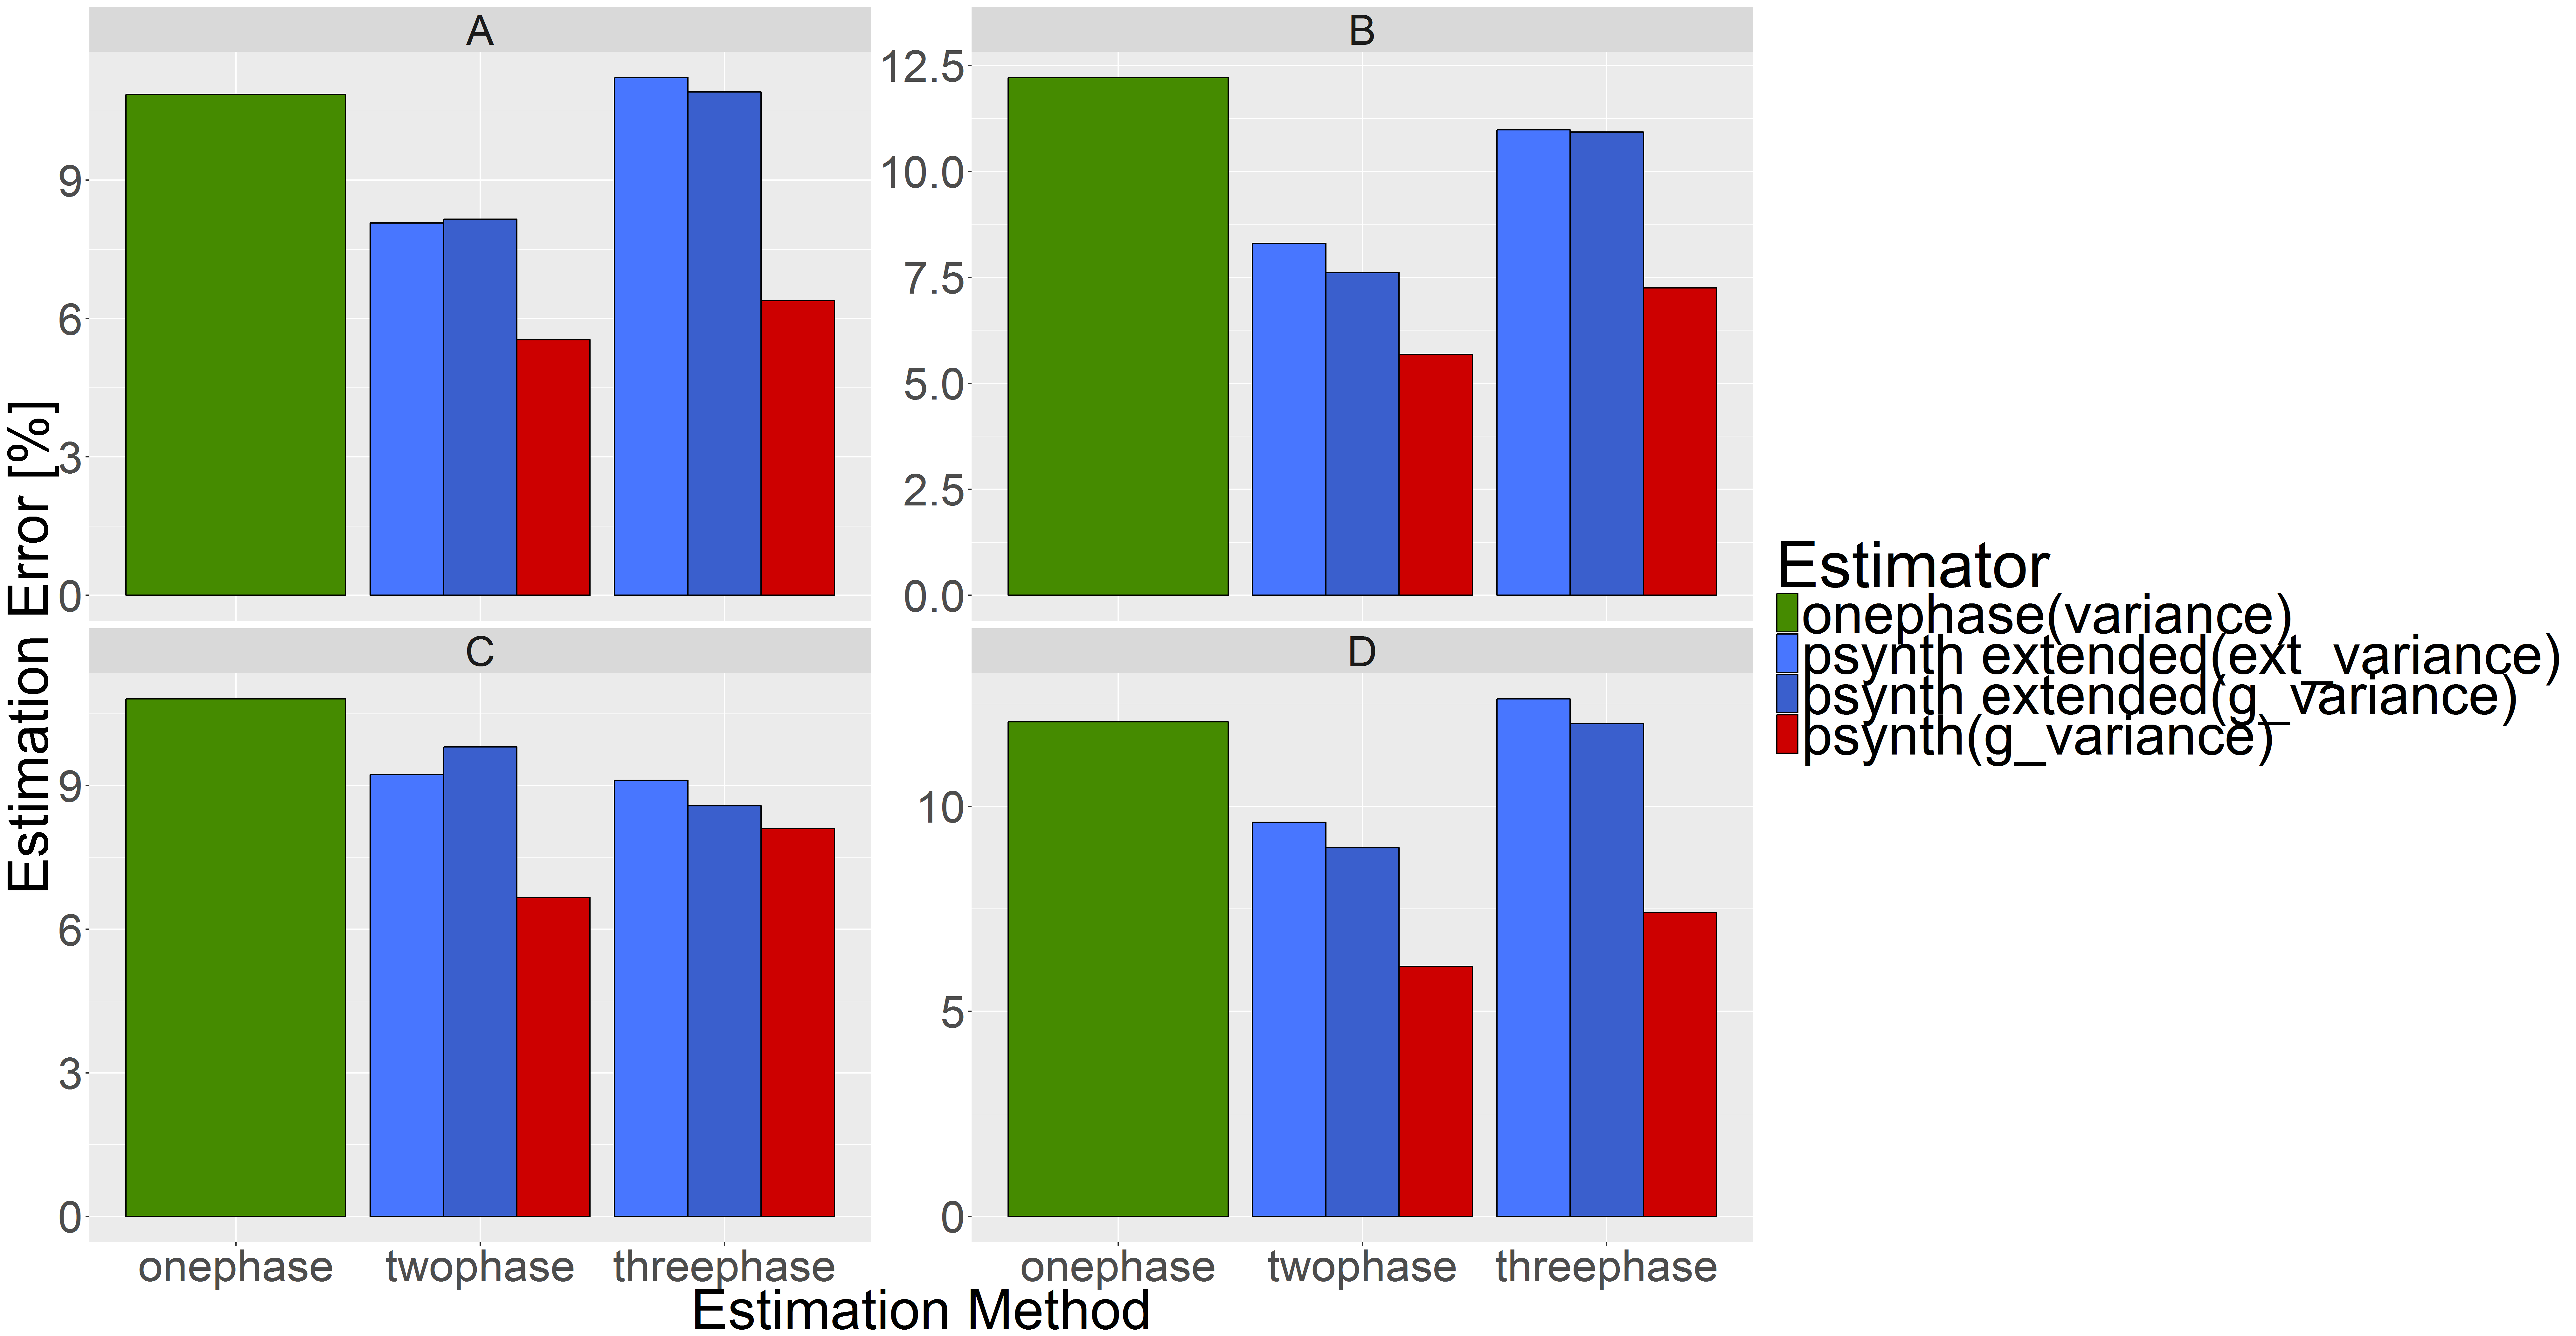
\includegraphics{Grafiken/Jstat_article/plot_error.png}}
\end{figure}

\newpage

Whereas the estimation errors are plotted by default, the point estimates and confidence intervals are returned when setting the argument \code{yvar = "estimate"}. Note that the graphics can arbitrarily be extended by additional \pkg{ggplot2} parameterizations.

\begin{small}
\begin{Schunk}
\begin{Sinput}
R> plot(grisons.sae.table, ncol = 2, yvar = "estimate") +
+    ylab("Timber Volume [m3/ha]")
\end{Sinput}
\end{Schunk}
\end{small}

\begin{figure}[h]
\centering
\resizebox{0.85\hsize}{!}{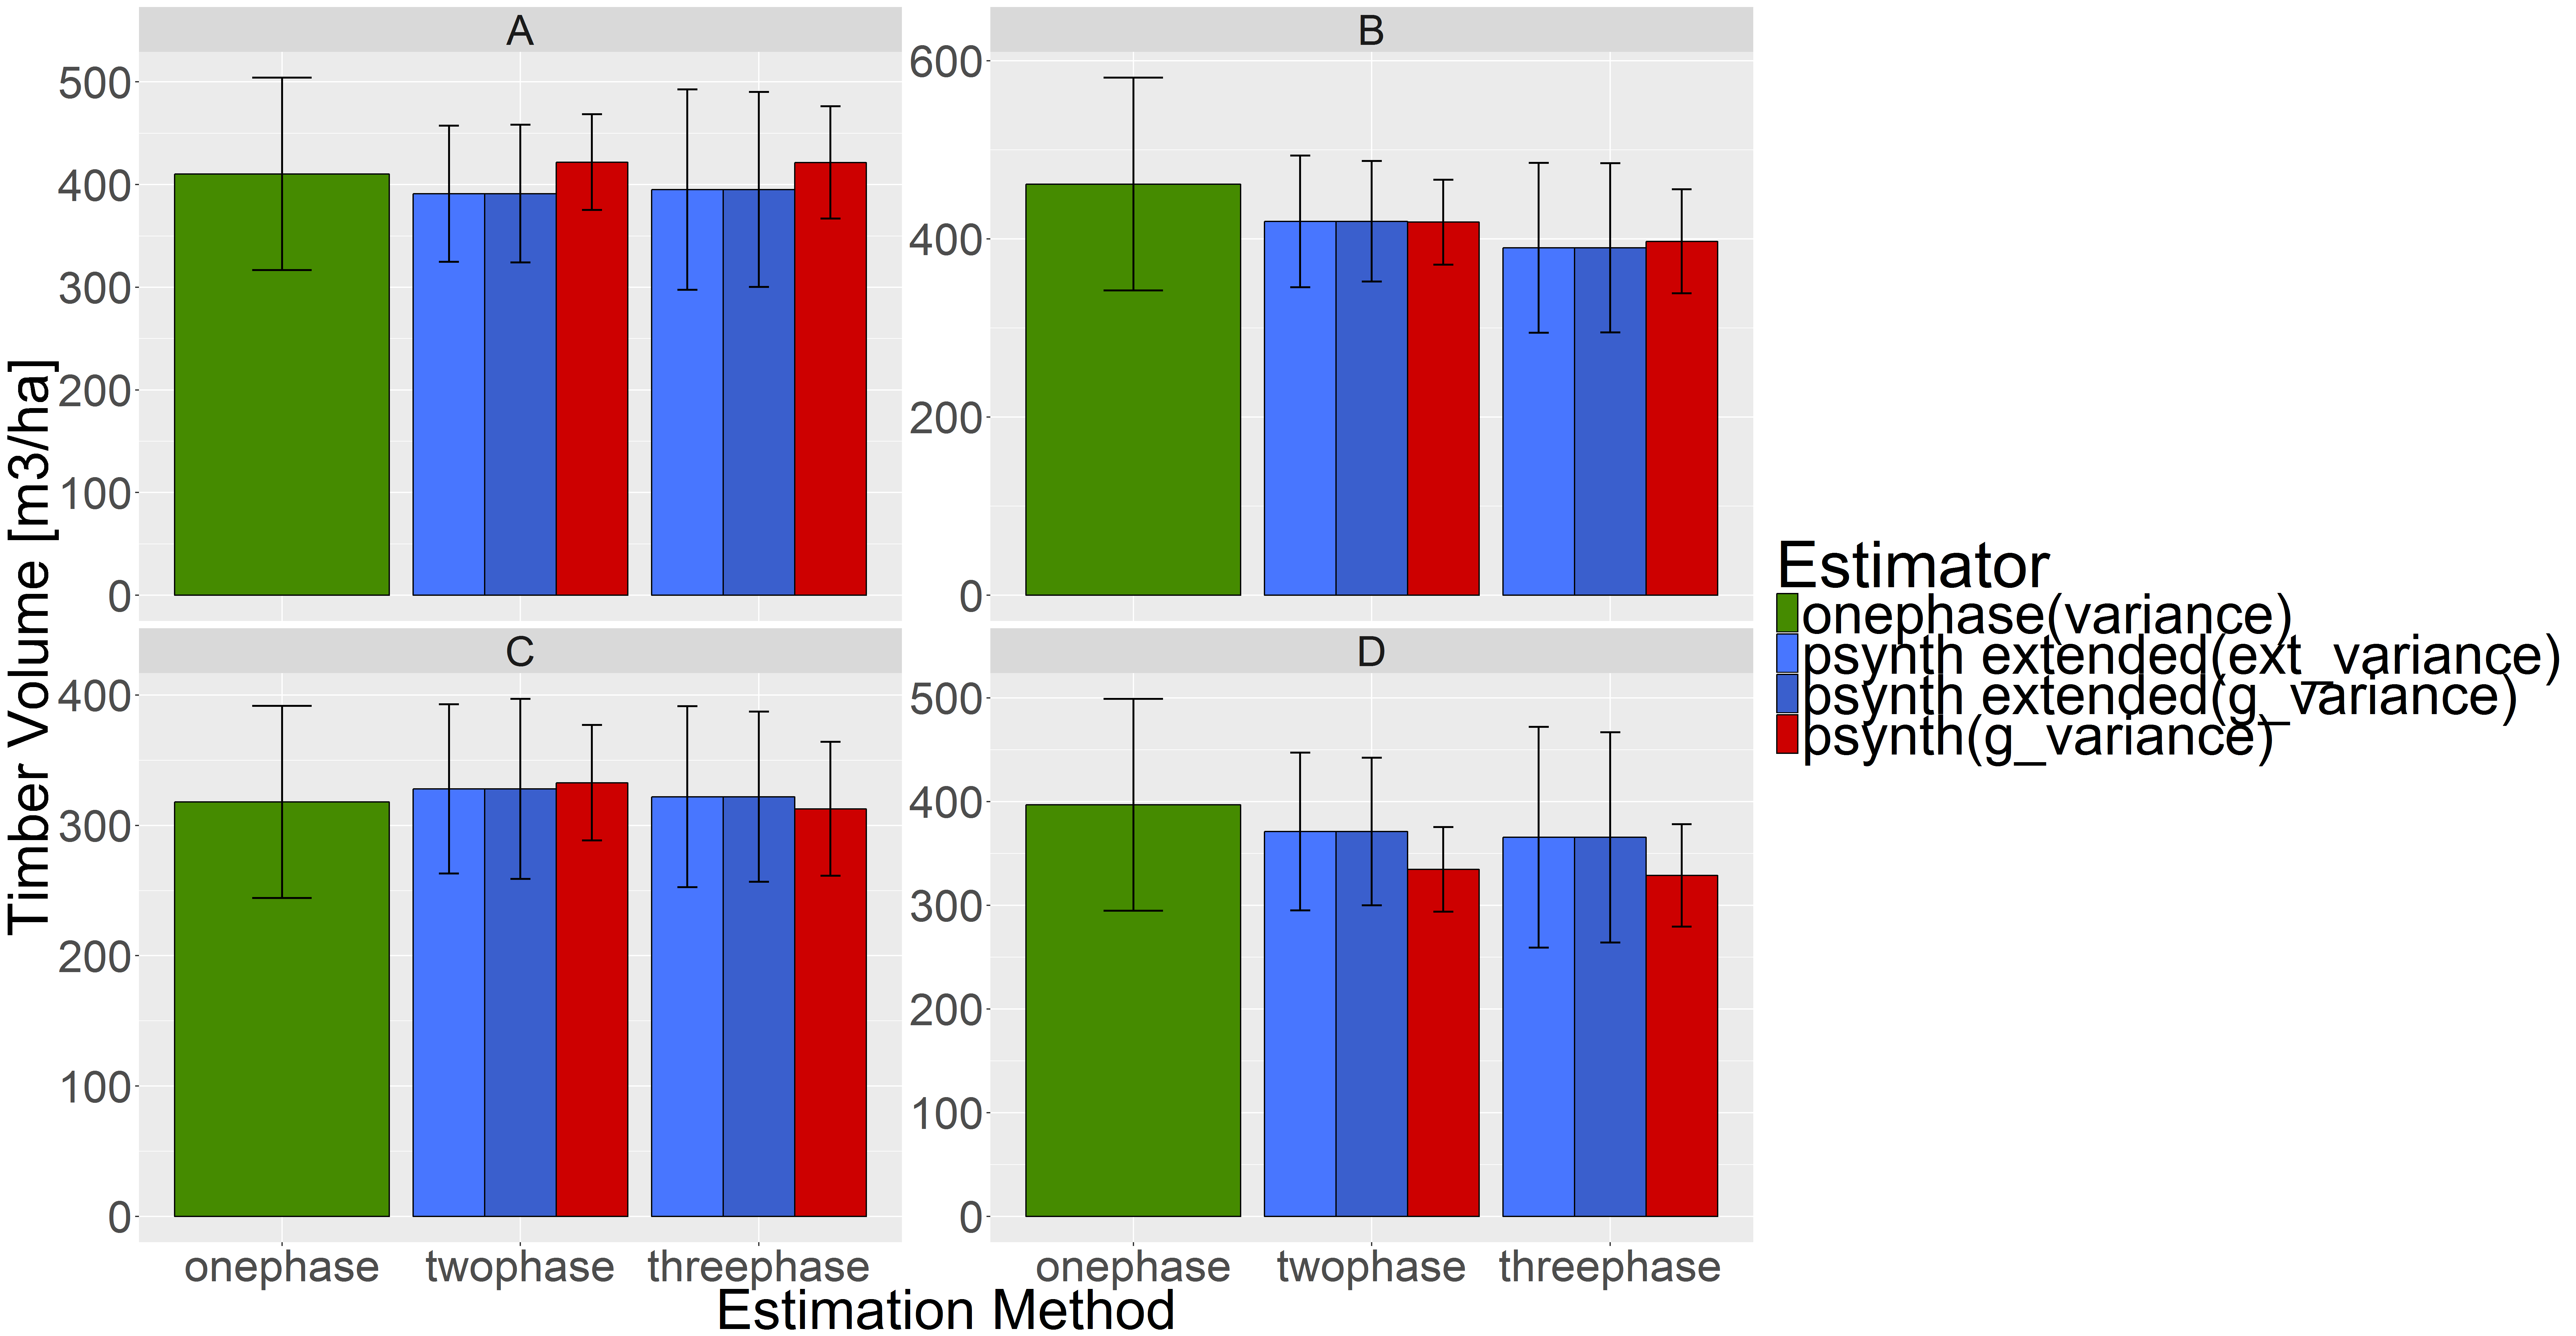
\includegraphics{Grafiken/Jstat_article/plot_est_ci.png}}
\end{figure}


%------------------------------------------------------------------------------------------------%
% ---------------------------------------- Future Plans---- ------------------------------------ %

\section{Future plans}
\label{sec:future}

The \pkg{forestinventory} package currently provides a fairly well-rounded toolkit for forestry inventorists to integrate auxiliary information into their estimates using the model-assisted methods under the design-based approach.  Although 32 combinations of inventory scenarios, estimators and sample designs are covered, there are still potential improvements planned for the future. As this is an open-source project, everyone is encouraged to give feedback and/or make contributions on the package's development page on GitHub \citep{github_forestinventory}. Currently planned extensions include:

\begin{itemize}
\item Implement parallel procedures for efficiently calculating many small areas.
\item Allow functions to accept objects of class \code{data.table} from the \pkg{data.table} package \citep{dt2017} to improve memory efficiency.
\item Enable the user to choose other types of models than linear regressions fitted with OLS.
\end{itemize}

%------------------------------------------------------------------------------------------------%
% ---------------------------------------- Acknowledgements ------------------------------------ %

\section*{Acknowledgements}

We want to express our gratitude to Prof. H. Heinimann (Chair of Land Use Engineering, ETH Zurich) for supporting this study and providing the possibility of working on the package. We also want to thank Daniel Mandallaz for his support in completing the range of the already published estimators in the frame of the three-phase small area estimators, as well as many helpful discussions and advice throughout the implementation of our package. Our thanks also go to Meinrad Abegg for proofreading the manuscript, and to the Amt f{\"u}r Wald und Naturgefahren of the Swiss canton of grisons for providing the example data.


	\clearpage
	\newpage
	\mbox{}
	\pagebreak
	\thispagestyle{empty}
	
%%% ------------------------------ Artikel 2 Regression Model ----------------------------------------- %%
\chapter{Combining canopy height and tree species map information for large scale timber volume estimations under strong heterogeneity of auxiliary data and variable sample plot sizes}
\label{chap:regmod}
{\large Andreas Hill$^1$, Henning Buddenbaum$^2$, Daniel Mandallaz$^1$}\\

\vspace{3cm}
\noindent
$^1$ETH Z\"urich\\Department of Environmental Systems Science, Universit\"atstrasse 16, 8092 Z\"urich, Switzerland \\

\noindent
$^2$Trier University\\Environmental Remote Sensing and Geoinformatics Department, Behringstrasse 21, 54286 Trier, Germany \\



\vspace{\fill}
\noindent
Submitted to:\\
\textit{European Journal of Forest Research} (in review).

\newpage
\thispagestyle{plain}
\renewcommand{\labelitemi}{--}
\begin{itemize}
	\item Henning Buddenbaum processed the airborne Laserscanning data and supported writing the manuscript.
	\item Daniel Mandallaz supported the statistical data analysis.
\end{itemize}

\clearpage
%%%%%%%%%%%%%%
%% Abstract %%
%%%%%%%%%%%%%%
\section*{Abstract}
\label{chap:regmod:Abstract}
A timber-volume regression model applicable to the entire forest area of the federal German state of Rhineland-Palatinate is identified using a combination of airborne laser scanning (ALS)-derived metrics and information from a satellite-based tree species classification map available on the federal state level. As is common in many forest inventory datasets, strong heterogeneity in the LiDAR data due to different acquisition dates and misclassifications in the tree species classification map had noticeable effects on the regression model's performance. This article specifically addresses techniques that improve the performance of ordinary least square regression models under such restricting conditions. We introduce a calibration technique to neutralize the effect of misclassifications in the tree species variable that originally caused a residual inflation of \changed{0.05} in adjusted $R^2$. Incorporating the calibrated tree species information improved the model accuracy by up to \changed{0.07} in adjusted $R^2$ and suggests the use of such information in forthcoming inventories. We also found that including ALS quality information as categorical variables within the regression model considerably mitigates issues with time lags between the ALS and terrestrial data acquisition and ALS quality variations (increase of \changed{0.09} in adjusted $R^2$). The model achieved an adjusted $R^2$ of 0.48 and a cross-validated root mean square error (RMSE$_{cv}$) of 46.7\% under incorporation of the tree species and ALS quality information, and was thus improved by \changed{0.12} in adjusted $R^2$ (5\% in RMSE$_{cv}$) compared to the simple model only containing ALS height metrics (adjusted $R^2$=0.36, RMSE$_{cv}$=51.7\%).


%------------------------------------------------------------------------------------------------%
% ---------------------------------- Introduction ---------------------------------------------- %

\section{Introduction}
\label{sec:intro}

Forest inventory methods are the primary tools used to assess the current state and development of forests over time. They provide reliable evidence-based information that is used to define and identify management actions as well as to adapt forest management strategies to both national and international guidelines. Two methods that have become particularly attractive are so-called \textit{double-sampling} \citep[\added{Ch. 5}]{mandallaz2008} and \textit{mapping} \changed{\citep{brosofske2014}} procedures. The core concept of these methods is to use predictions of the terrestrial target variable at additional sample locations where the terrestrial information has not been gathered. These predictions are produced by models that use explanatory variables derived from \textit{auxiliary data}, commonly in the form of spatially exhaustive remote sensing data in the inventory area. \added{Especially models to predict timber volume based on airborne laser scanning (ALS) have been extensively investigated for a long time \citep{naesset1997}.} The specific scope of double-sampling is to enlarge the terrestrial sample size by a much larger sample of predictions of the target variable in order to gain higher estimation precision without performing additional expensive terrestrial measurements. Model-dependent and design-based regression estimators are used in a broad range of double sampling concepts and methods \citep{gregoire2007, kohl2006, schreuder1993, saborowski2010, mandallaz2013a, mandallaz2013c} and have been applied to existing inventory systems \citep{breidenbach2012, vonLuebke2014, mandallaz2013b, magnussen2014, massey2014a}. While double-sampling methods provide reliable estimates for a given spatial unit, e.g. a forest district, they do not provide information about the spatial distribution of the estimated quantity within this area. For this reason, the same modeling technique used in double-sampling procedures has also been intensively used to produce exhaustive prediction maps that provide pixelwise estimations of a target variable in high spatial resolution \citep{bohlin2017, latifi2010, tonolli2011, hill2014, nink2015}.\par

To allow for an area-wide application of the prediction model, both double sampling and mapping methods require that the remote sensing data are available over the entire inventory area. This is usually not a limiting factor in \textit{small-scale} applications. In the optimal case, the remote sensing data are in principle collected in accordance to the specific study objective. Quality standards that have often been addressed are that \textit{a)} the remote sensing data should be acquired close to or even at the time of the terrestrial inventory in order to ensure best possible comparability between the target variable on the ground and the remote sensing derived variables \citep{mcroberts2015}; \textit{b)} the remote sensing technology and its spectral and spatial resolution should be chosen according to the modelling purpose \citep{kohl2006}; and \textit{c)} the variation in quality of the remote sensing data over the inventory area should be minimized in order to avoid artificial noise in the data \citep{naesset2014inmaltamo}. Despite the increasing availability and decreasing costs of remote sensing data \citep{white2016}, these quality standards of the remote sensing data can often not be guaranteed for \textit{large-scale} applications \citep{maack2016}, and trade-offs must be accepted \citep{jakubowski2013}. The prime objective is then to produce the best possible prediction model given the restrictions imposed by the available remote sensing information. The exploration of scarcely used remote sensing products and the optimization of prediction models under severe quality restrictions in the remote sensing data are thus one of the challenges in large-scale model-supported inventory applications.\par

Among the still rarely used remote sensing data in large scale applications, the integration of tree species information in prediction models - especially for timber volume estimation - has been stated as some of the most promising but often missing information \citep{koch2010, white2016}. As timber volume estimations on the single tree level in forest inventories are often based on species-specific biomass and volume equations \citep{husmann2017,zianis2005}, the application of species-specific models is expected to be a key factor for improving estimation precision \citep{white2016}. \changed{This has been supported by studies from \citet{breidenbach2008} who achieved a substantial improvement in accuracy of their timber volume prediction model when including a variable estimating the deciduous proportion derived from leaf-off ALS data. Similar gains in model performance were also reported by \citet{straub2009} and \citet{latifi2012} who used broadleaf and coniferous information based on color infrared orthophotos as a categorical explanatory variable. However, studies that explore the use of more species-specific information (i.e. a further discrimination of tree species) as explanatory variables have been rare. Further investigations are thus necessary especially in countries whose forests are characterized by a larger variety of tree species that may also occur in mixed and uneven-aged stands \citep{mcroberts2010}.} The area-wide tree species information in most studies was obtained from satellite and airborne remote sensing sensors based on automatic classification methods. Whereas the presence of misclassifications has already been addressed \citep{latifi2012}, an issue that has so far been neglected is how misclassifications actually affect the prediction model \citep{gustafson2003}.\par

A frequently encountered problem in large scale forest inventories is the lack of temporal synchronicity between the remote sensing acquisition and the terrestrial survey. As a result, the available remote sensing data often exhibit notable time-lags with respect to the date of the terrestrial inventory. This has often been addressed as a major drawback, especially for the application of design-based change estimation \citep{massey2015b}.\par

Our study is embedded in the current implementation of design-based regression estimators \citep{mandallaz2013a, mandallaz2013b, mandallaz2013c} for estimating the standing timber volume within the state and communal forest management units over the entire state of Rhineland-Palatinate (RLP, Germany). With respect to this overall objective, the aim of this study was to derive an ordinary least square (OLS) regression model to generate predictions of the standing timber volume associated with a sample location of the Third German National Forest Inventory (BWI3) over the entire state and communal forest area (6155 km$^2$). A merged ALS dataset from different acquisition years and a satellite-based tree species classification map for the five main tree species in RLP was available for the entire inventory area and consequently used to derive predictor variables. The major limiting factors for using these data in a regression analysis are \textbf{(i)} variation in the ALS data quality as well as time-lags of up to 10 years between the ALS acquisitions and the terrestrial survey, \textbf{(ii)} misclassifications in the tree species classification map and \textbf{(iii)} the ambiguous choice of a suitable extraction area (\textit{support}) for all remote sensing information under angle count sampling in the terrestrial survey (variable sample plot sizes). For this reason, we address the following specific research questions:

\begin{enumerate}
	\setlength\itemsep{1em}
	\item How can tree species map information be optimally used within a regression model that predicts timber volume? What effects do misclassifications have on the predictions and how can these effects be minimized?
	\item What are the effects of quality restrictions and substantial time lags between the ALS- and terrestrial data acquisition on the regression model and how can these effects be mitigated?
	\item Does support size influence model accuracy? What is the optimal support size and what are the determining factors?
\end{enumerate}

%---------------------------------------------------------------------------------------------------------%
% ---------------------------------- Materials and Methods ---------------------------------------------- %

\section{Materials and Methods}
\label{sec:MatMeth}

% ----------------------------------------------------------------------- %
% ----------------------------------------------------------------------- %
\subsection{Study Area}
\label{sec:studyarea}

The German federal state Rhineland-Palatinate (RLP) is located in the western part of Germany and borders Luxembourg, France and Belgium (figure \ref{fig:Study Area}). With 42.3\% (appr. 8400 km$^2$) of the entire state area (19850 km$^2$) covered by forest, RLP is one of the two states with the highest forest coverage among all federal states of Germany \citep{bwi3}. \added{The forest area of RLP is divided into three ownership classes, i.e. state forest (27\%), communal forest (46\%) and privately owned forest (27\%).} The most frequent tree species in RLP are European beech (\textit{Fagus sylvatica}, 21.8\%), oak (\textit{Quercus petrea} and \textit{Quercus robur}, 20.2\%), Norway spruce (\textit{Picea abies}, 19.5\%), Scots pine (\textit{Pinus sylvestris}, 9.9\%), Douglas fir (\textit{Pseudozuga menziesii}, 6.4\%), European larch (\textit{Larix decidua}, 2.4\%) and Silver fir (\textit{Abies alba}, 0.7\%). The share of broadleaf tree species is 58.7\%. The forests of RLP further exhibit heterogeneous structures \citep{bwi3}: around 82\% of the forest area in RLP are mixed forest stands (i.e. at least two different tree species occur in the same stand) and 69\% of the forest area exhibit a multi-layered vertical structure. While the average tree age is around 80 years, most of the forest area (20\%) is occupied by trees between 40 and 60 years of age, whereas 27\% of the trees are older than 100 years. Spatially variable climate conditions have a strong influence on the local growth dynamics as well as tree species composition and create a large variety of forest structures, ranging from characteristic oak coppices (Moselle valley), pure spruce, beech and Scots pine forests (e.g. Hunsr{\"u}ck and Palatinate forest) to mixed forests comprising variable proportions of oak, larch, spruce, Scots pine and beech. Accordingly, RLP has been divided into 16 bioclimatic growing regions that form homogeneous areas with respect to the afore mentioned characteristics \citep{gauer2005}.

\begin{figure}[H]
	\centering
	\resizebox{0.65\hsize}{!}{\includegraphics*{Grafiken/Regmod_article/terr_sampledesign_bw.png}}
	\caption{Spatial distribution of the \bwi{} cluster samples over Rhineland-Palatinate}
	\label{fig:Study Area}
\end{figure}

% ----------------------------------------------------------------------- %
% ----------------------------------------------------------------------- %
\subsection{Terrestrial Inventory Data}
\label{sec:terrdata}
The German National Forest Inventory (NFI) is carried out over the entire forest area of Germany in reoccurring time periods of 10 years. The most recent inventory (\bwi{}) has been conducted in the years 2011 and 2012. In this framework, Rhineland-Palatinate is covered by a 2x2 km grid that defines the sample locations for the terrestrial survey. A sample unit consists of four sample locations (also referred to as \textit{sample plots}) that are arranged in squares (so called \textit{clusters}) with a side length of 150 metres (figure \ref{fig:Study Area}). The number of plots per cluster can however vary between 1 and 4 depending on forest/non-forest decisions on the plot level \citep{bwi3_aufn}. In the field survey of the \bwi{}, sample trees for timber volume estimations are selected according to the angle count sampling technique \citep{bitterlich1984}, using a basal area factor ($BAF$) of 4 that is respectively adjusted for boundary effects at the forest border \citep{bwi3_aufn}. A further selection criterion for a tree to be recorded is a diameter at breast height ($dbh$) of at least 7 cm. \added{This sampling technique was applied to 8092 sample plots (2810 clusters) in RLP, resulting in the collection of 56561 sample trees for which the dbh, the tree diameter at 7 m ($D7$) and the tree species were recorded for all trees. Tree height measurements were conducted only for a subset of all sample trees and used to predict the height for the remaining sample. During the last inventory, all plot center positions were remeasured with differential global positioning system (DGPS) technique. Knowledge about the exact plot positions were considered crucial to provide optimal comparability between the terrestrial observations and the information derived from the auxiliary data. A detailed analysis by \citet{lambrecht2017} indicated that horizontal DGPS errors do not exceed 8 meters for 80\% of all plots in RLP. For 162 plots, the DGPS coordinates were replaced by their former target coordinates due to missing or implausible values.} In order to derive a volume estimation for each sample tree, the \bwi{} estimates a taper curve for each sample tree by calibrating the random effects term of linear mixed-effects taper models with the set of diameters and corresponding height measurements taken from the respective sample tree \citep{kublin2013}. The integration of the derived taper curves consequently lead to a volume prediction for each sample tree. \changed{Since the overall objective of the study was to subsequently use the identified regression model for design-based timber volume estimations of state and communal forest management units, we already restricted the sample plots used for modeling to the state and communal forest area (73\% of the entire forest area of RLP). This provides the advantage that when the regression model is used as an \textit{internal model} in design-based estimators, the model predictions hold the assumption on the residuals to be zero on average over the state and communal forest area by construction of OLS technique \citep{mandallaz2013a, mandallaz2013b, mandallaz2013c}.} The dataset of this study hence comprised 5791 plots (2055 clusters). For this sample, the timber volume density per hectare on plot level, $Y(x)$, was calculated according to the formula of one-phase one-stage sampling \citep[\added{Ch. 4.2}]{mandallaz2008}. The timber volume density per hectare on plot level was used as the response variable in the regression analysis.

% table of field measured values:

\begin{table}[ht]
	\centering
	\caption{Descriptive statistics of the forest observed on NFI sample plots located iwithin communal and state forest area (n=5791).}
	\label{tab:fieldata}
	\begin{tabular}{lllrrr}
		\hline
		Variable & Mean & SD & Maximum \\ 
		\hline
Timber Volume (m$^3$/ha) & 300.86 & 195.55 & 1375.31 \\
Mean DBH (mm) & 354.90 & 137.22 & 1123.20 \\
Mean height (dm) & 239.60 & 72.43 & 497.43 \\
Mean stem density per hectare & 101.00  & 114.01 & 1010.31 \\
\hline
\hline
\end{tabular}
\end{table}

% ----------------------------------------------------------------------- %
% ----------------------------------------------------------------------- %
\subsection{Auxiliary Data}
\label{sec:auxinfo}

% ----------------------------------------------------------- %
\subsubsection{ALS Canopy Height Model}
\label{sec:chm}

% new version:
Between 2003 and 2013, the topographic survey institution of RLP acquired airborne laser scanning (ALS) data over the entire state of RLP at leaf-off condition (Figure \ref{abb:lidaryears}). The objective of this campaign was to derive a countrywide digital terrain and surface model based on the acquired ALS point clouds. During the extended acquisition period, airborne laser scanning technology and data quality evolved significantly. The tiles recorded in 2002 and 2003 have a rather poor quality with about only \changed{0.04 points per m$^2$}, while more recently acquired datasets \changed{contained about} \changed{5 points per m$^2$}. \changed{The data was delivered as two separate datasets comprising the Vegetation First Pulse (VEF) and Ground (GRD) points. All point clouds were stored as three-column (easting, northing, and height above sea level) ASCII files in tiles of 1 km$^2$. In order to create a surface model (DSM) in a given raster resolution, the highest point of the combined VEF and GRD dataset was identified in each raster cell and saved as a thinned surface point cloud. For the elevation model (DEM), the mean of all GRD points in the cell was calculated, and the result was saved as a thinned ground point cloud. The thinned point clouds were then aggregated to larger tiles and interpolated to raster images using a Delauney interpolation in the Matlab software \citep{matlab}. The resulting DSM and DEM raster sets were then subtracted from each other to calculate a canopy height model (CHM) in raster format, providing discrete information about the canopy surface height of the entire forest area of RLP in a spatial resolution of 5 meters. The thinning process led to much smaller datasets that could be processed in larger tiles and considerably lowered processing times compared to the original dense point clouds. Since the data was recorded in leaf-off condition, the original point clouds contained many returns from within the crowns of deciduous trees. The thinned dataset provided the advantage that those measurements did not skew the vegetation height estimate in the final CHM.}\par

As explanatory variables, the mean canopy height (\textit{meanheight}) and the standard deviation ($stddev$) were calculated as the mean and standard deviation of all raster values within a predefined circle (i.e. \textit{support} of the explanatory variable, see section \ref{sec:supp}) around each sample plot center. \changed{In order to correct for edge effects at the forest border, each support area was previously intersected with the state and communal forest area, which was defined by a polygon mask provided by the forest service (figure \ref{fig:sf2}). Restricting the support area and thus the evaluation of the auxiliary data to the forest area is a means to optimize the coherence between explanatory variables computed at the forest boundary and the corresponding terrestrial response variable \citep{mandallaz2013b}.} The tree height is one prominent predictor variable in the taper functions of the \bwi{} that are used to calculate a timber volume value for each sample tree \citep{kublin2003, kublin2013}. A visual inspection of the tree volumes of all sample trees collected in the \bwi{} within RLP against their tree heights also revealed the characteristic shape of an allometric relationship between these variables (Online Resource 1). It was hypothesized that this relationship on single-tree level is also apparent on the aggregated level of a sample plot and cluster, and can be used within the frame of regression modeling.\par
The strength of correlation between \textit{meanheight} and timber volume on plot level was expected to show high variation according to the mentioned time-lag up to 10 years between ALS acquisition and terrestrial survey. The quality of the height information was also expected to vary according to changing sensor technologies and different point densities used over the years. For these reasons, the ALS acquisition year (\textit{ALSyear}) for each sample plot was considered as a potential categorical explanatory variable to explain the variation in the data introduced by these factors. For this purpose, the acquisition year \textit{2008} was further divided into \textit{2008} and \textit{2008\_1}. In the latter, the data quality turned out to be very poor due to sensor failures during the acquisition. Additionally, the years \textit{2006} and \textit{2007} as well as \textit{2012} and \textit{2013} were pooled in order to increase the number of observations per factor level for modelling reasons. As a result, the \textit{ALSyear} variable comprised nine categories (\textit{2002}, \textit{2003}, \textit{2007}, \textit{2008}, \textit{2008\_1}, \textit{2009}, \textit{2010}, \textit{2011} and \textit{2012}).

\begin{figure}[H]
	\centering
	\resizebox{0.45\hsize}{!}{\includegraphics*{Grafiken/Regmod_article/lidar_years_quality.png}}
	\caption{Separate ALS acquisitions in Rhineland-Palatinate over the years. The colors also indicate the quality of the data: \textit{light}: low point densities (0.04/$m^2$), \textit{dark}: high point densities ($>$4/$m^2$). \added{Blue semitransparent layer: state and communal forest area.}}
	\label{abb:lidaryears}
\end{figure}



% ----------------------------------------------------------- %
\subsubsection{Tree Species Classification Map}
\label{sec:tspecclass}

A countrywide satellite-based classification map of the five main tree species (European beech, Sessile and Pedunculate oak, Norway spruce, Douglas fir, Scots pine) described in \citet{stoffels2015} was used to derive tree species information on sample plot level. The classified tree species map has a grid size of 5 meters and predicts five of the seven tree species that are used in the \bwi{} taper functions \citep{kublin2013} to calculate the timber volume of a sample tree. Due to unavailable satellite data for the classification, the tree species map excluded one patch with an area of 415 km$^2$ in the south-west part of RLP, and two further patches with an area of 76 km$^2$ and 100 km$^2$ in the northern part \citep{stoffels2015}. The tree species information was consequently missing for \changed{411} (7\%) of the 5791 sample locations.

\subsubsection*{Prediction of main plot tree species}

A visual inspection of all \bwi{} sample trees of RLP suggested that a stratification of the relation between tree height and timber volume according to these seven tree species may provide a considerable reduction in variation within the tree species groups (Online Resource 1). This led to the hypothesis that this tree species specific signal might also be apparent on sample plot and cluster level and can consequently be used to increase the accuracy of the prediction model. Based on the tree species classification map, the main tree species of each sample plot was calculated as an additional categorical explanatory variable ($treespecies$) with six categories following a similar approach as \citet{latifi2012}: one of the five tree species was assigned as the main plot tree species if its proportion within the edge-corrected support around the sample location exceeded a predefined threshold. If this threshold was not reached by any of the five tree species, the respective sample plot was assigned the category 'Mixed'. \changed{We hypothesized that the choice of the threshold-value might have an influence on the resulting classification accuracy and the regression model accuracy (section \ref{sec:modval}). We thus investigated the application of 5 threshold settings, i.e. 0\%, 50\%, 60\%, 80\% and 100\%.}
\par


\subsubsection*{Calibration}

\changed{Our analyses revealed that the prediction of the main tree species for a sample plot can be subject to misclassifications (section \ref{sec:supp_tspec_res}). Errors in the explanatory variables of linear regression models can however lead to a bias of the regression coefficients in the direction of zero due to an artificial introduction of noise \citep[Ch. 3]{carroll2006}. This can cause an inflation of the residual variance and a consequent decrease of the model accuracy \citep{magnussen2010}. In case of classification, the impacts of misclassifications on the model properties are even harder to predict \citep[Ch. 3]{gustafson2003}. While errors in the explanatory variables do not affect the unbiasedness of the estimators in the design-based framework, a reduction or elimination of the classification errors could provide an improvement of the regression model accuracy and thereby potentially lead to smaller prediction and estimation errors. We therefore addressed the effect of misclassifications in the \textit{treespecies} variable categories as well as means to correct these errors.\par
	
	We transferred the concept of \textit{regression calibration} as known from classical measurement error statistics \citep{carroll2006} to the problem of misclassifications in the \textit{treespecies} variable. In regression calibration, one considers an error-prone explanatory variable $W$ that can be measured in high quantity, whereas $X$ constitutes the same but error-free variable whose determination is however very expensive. In order to yield a corrected or less error-prone version of $W$, one can define a calibration model $f_{calmod}(X,W)$ that predicts $X$ as a function of $W$. After calibration on a training set, $f_{calmod}()$ can then be applied to any observed $W$ and yields the corrected, less error-prone variable $W_{calib}$. Using $W_{calib}$ instead of $W$ in the regression model then asymptotically provides an unbiased estimate of the regression coefficients and thus corrects for the attenuation to zero.\par
	
	We transferred this concept by using a random forest algorithm \citep{breiman2001} as calibration model. We considered the main tree species of the sample trees at each plot location $x$ as the error-free variable $treespecies_{terr}$, that would also yield the highest model accuracies when used as predictor variable. The objective of the calibration model was thus to provide an improved classification accuracy of each predicted main plot tree species category with respect to $treespecies_{terr}$. The calibration model was considered to correct for potential systematic misclassifications and thus minimize the effect of misclassifications on the regression model when substituting the uncalibrated with the calibrated $treespecies$ variable. The random forest algorithm is a machine learning algorithm that grows a large number of decorrelated classification trees by considering only a subset of all provided predictor variables for each split. In the case of classification, new data are thus predicted by aggregating the predictions of all trees using a majority vote. We calibrated the random forest algorithm ($f_{RF}$) with a set of $p$ predictor variables that comprised the initial prediction of the main plot tree species (\textit{treespecies}), the mean canopy height (\textit{meanheight}) and standard deviation ($stddev$) derived from the CHM, the proportion of coniferous trees estimated from the tree species classification map ($prop.conif$) and the bioclimatic growing region ($wgb$) at the sample location (equation \ref{eq:calibmod}). An advantage for using those explanatory variables in the calibration model was that they also provided explanatory power in the regression model. This approach thus saved computation time and minimized data storage. The calibration model was implemented using the random forest algorithm \citep{liaw2002} in the statistical software $R$ \citep{R}. The algorithm was grown with 2000 trees, considering $\sqrt{p} \approx$ 3 of the predictors for each split.\par
	
	\begin{equation} \label{eq:calibmod}
	\begin{split}
	treespecies_{terr}(x) = f_{RF}(&treespecies, meanheight, \\
	&stddev, prop.conif, wgb)
	\end{split}
	\end{equation}
	
	The calibration model was subsequently applied to the entire dataset. We then investigated the effect on the regression model performance (regression coefficients, model accuracy) when substituting the calibrated (less error-prone) for the uncalibrated (most error-prone) variable, and likewise for the actual (error-free) main plot tree species derived from the sampled trees of the respective sample plot under identical threshold settings.\par
	
}

% ----------------------------------------------------------------------- %
% ----------------------------------------------------------------------- 
\subsection{Choice of Support under Angle Count Sampling}
\label{sec:supp}

One characteristic of angle count sampling applied in the \bwi{} is that a sample plot does not have a fixed radius in which trees are selected (\textit{fixed-radius plot}), but each tree generates an individual radius from the plot center depending on its diameter at breast height (\textit{variable-radius plot}). This tree-individual radius is known as the \textit{limiting distance} from the plot center where the tree would still be included in the sample. A consequence of the absence of a fixed plot radius is the question about the optimal support \citep{hollaus2007}, i.e. the spatial extent around the plot center in which the auxiliary information is evaluated and transformed into an explanatory variable. It has widely been hypothesized that the best relationship between the target variable on the ground and any explanatory variable derived from the auxiliary information is obtained if the support is spatially identical to the sample plot extent. In case of angle count sampling, an individual extent for each sample plot can be approximated by regarding the maximum limiting distances of its sample trees as the outer plot radius. However, many design-based applications under double-sampling do not allow for a between-plot change of the support for a specific explanatory variable \citep{mandallaz2013c, mandallaz2013a}.\par
For this reason, the task is to find a unique support for each auxiliary information that leads to the best overall model accuracy. \citet{deo2016} conducted extensive analysis to identify optimal supports for modelling standing timber volume for \textit{variable-radius plot} designs in conifer forests. They analysed 24 different radii (i.e. circular supports) in which they extracted 57 metrics from a ALS derived point cloud with an average point density of 18 pulses per square meter. They successively evaluated the prediction performance of each support size by using the ALS metrics in a random forest algorithm and comparing the resulting model accuracies. In order to identify the best-performing supports for our explanatory variables, we followed a similar approach. The explanatory variables were calculated using $individual$ (i.e. plot-varying) supports ($ind$), i.e. an individual support radius was used for each plot according to the maximum limiting distance of all sample trees associated to the respective sample plot. We then compared the model accuracies achieved by the individual supports against the model accuracies from a set of $fixed$ (i.e. non plot-varying) supports. The extents of the fixed supports were chosen from the cumulative distribution function (ECDF) of the maximum limiting distances of all 5791 sample plots of the analysed forest area (Fig. \ref{fig:sf1}). We considered the $25^{th}$ ($q25$, 9 meters), $50^{th}$ ($q50$, 12 meters), $80^{th}$ ($q80$, 15 meters) and the $100^{th}$ ($q100$, 38 meters) percentiles, resulting in support radii of 18, 24, 30 and 76 meters (Fig. \ref{fig:tspec_supps}). While in this study we also used circular supports to extract the auxiliary information, also other support-shapes are possible (e.g. rectangles, hexagons). We also want to emphasize that the use of different support sizes for each explanatory variable is perfectly valid in the infinite population framework of design-based estimators \citep{mandallaz2013c, mandallaz2013a}.

%\begin{figure}[h]
%	\centering
%	\subcaptionbox{ECDF of maximum limiting distances of all \bwi{} sample locations in RLP \label{fig:sf1}}{
%		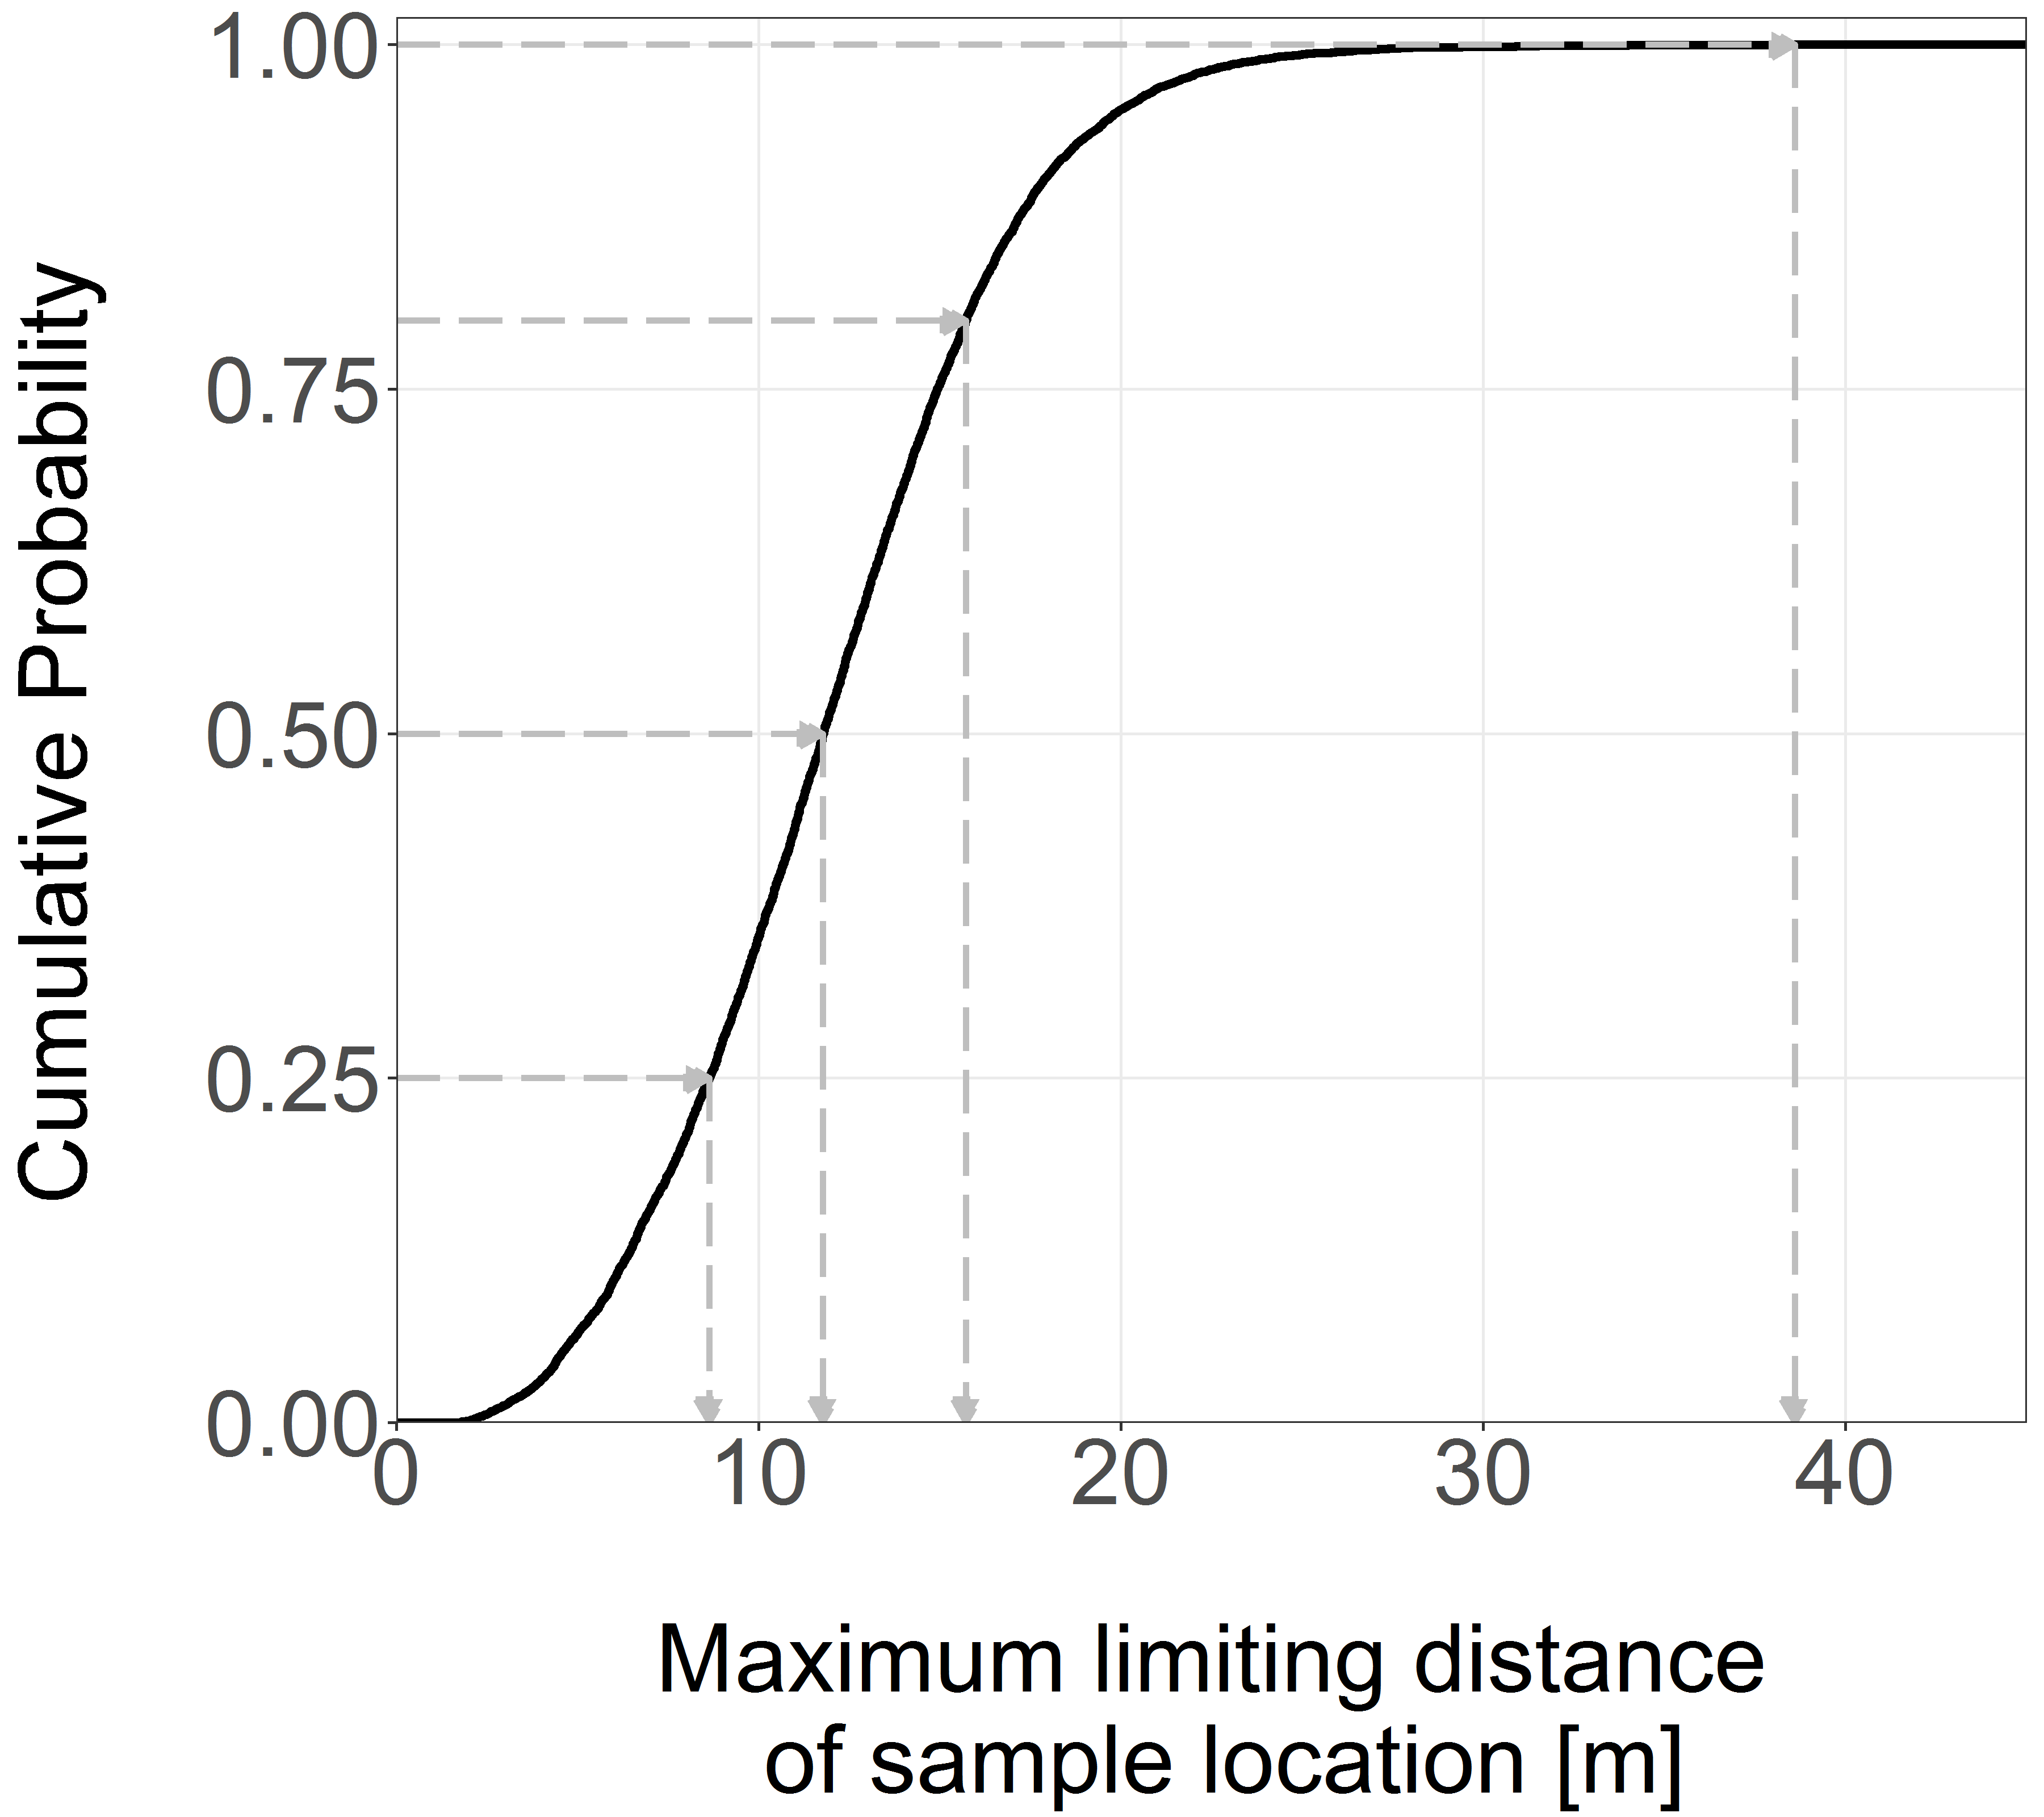
\includegraphics[width=0.36\textwidth]{Grafiken/Regmod_article/cdf_maxri.png}%
%	}\par\medskip
%	\subcaptionbox{Circular supports used to extract explanatory variables around sample locations. \textit{Dash dot dot line}: q100, \textit{dash dot line}: q80, \textit{dot dot line}: q50, \textit{dot line}: q25, \textit{solid line}: individual support, \textit{triangles}: sample trees \label{fig:sf2}}{
%		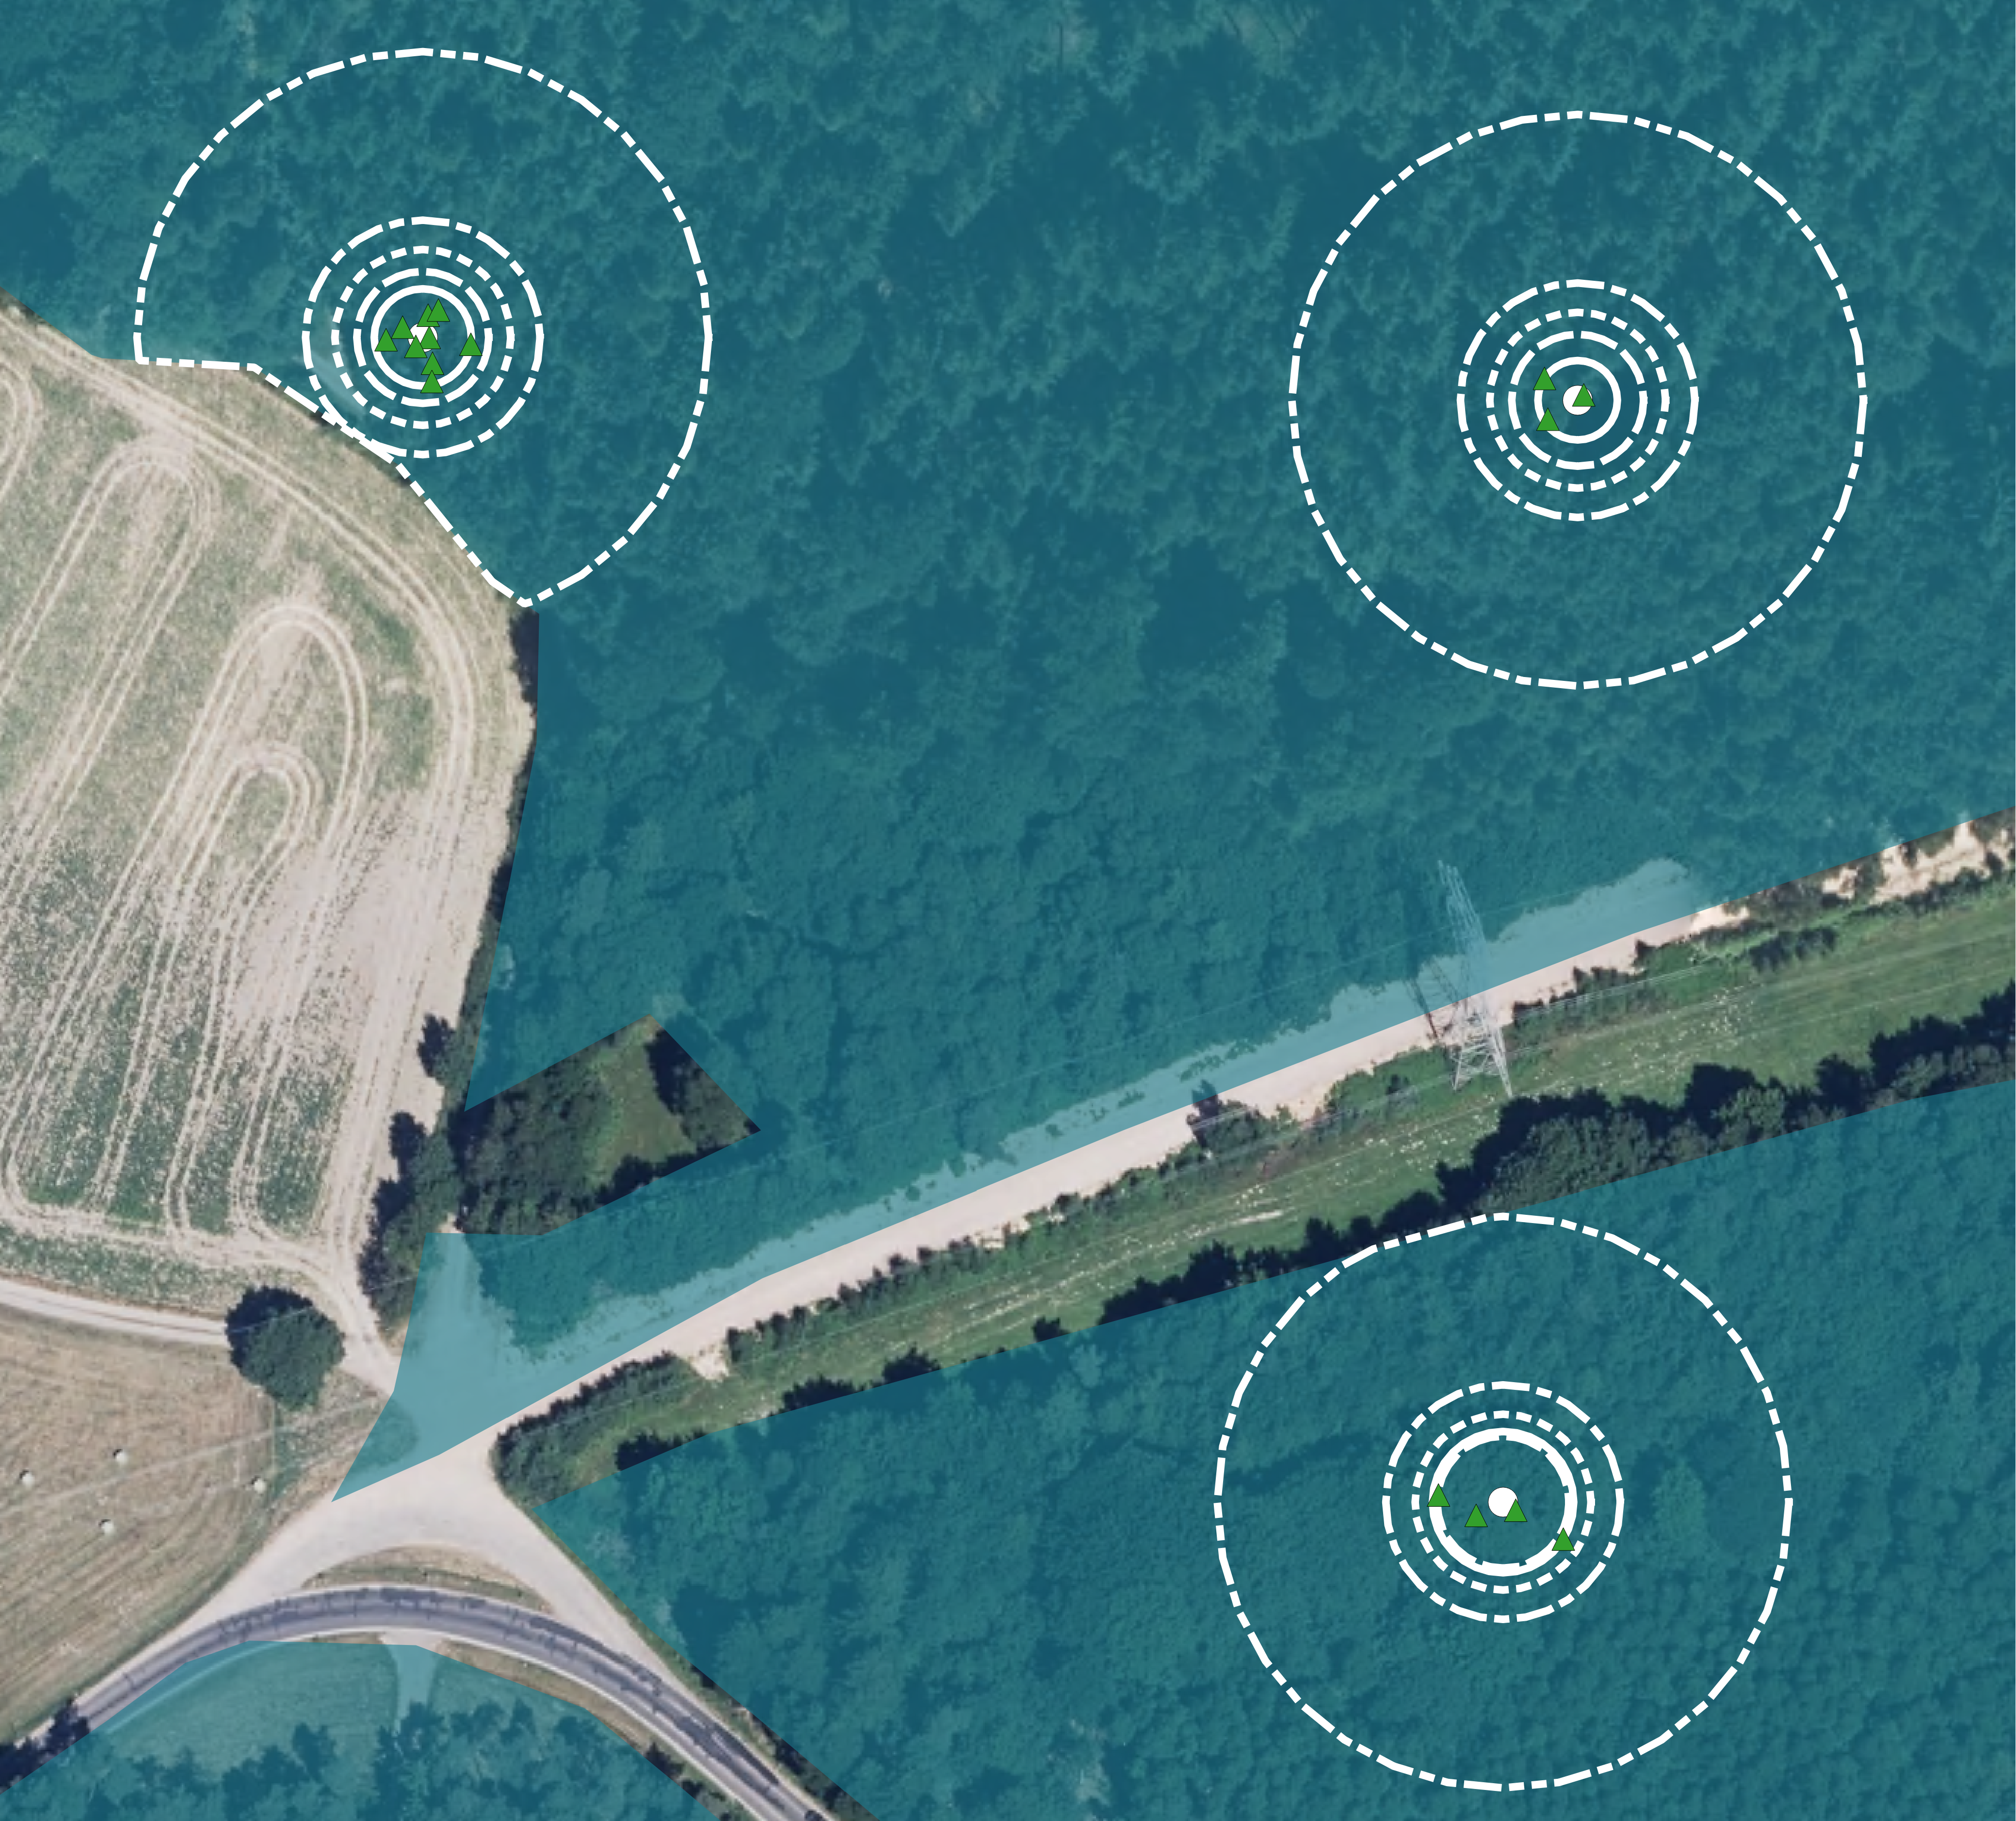
\includegraphics[width=0.36\textwidth]{Grafiken/Regmod_article/choice_of_support.png}
%	}\par\medskip
%	\caption{Identification (\textit{a}) and visualization (\textit{b}) of potential supports used for calculating the predictor variables on plot level}
%	\label{fig:tspec_supps}
%\end{figure}


\begin{figure}[h]
	\begin{subfigure}[t]{0.5\textwidth}
		\centering
		\resizebox{0.85\hsize}{!}{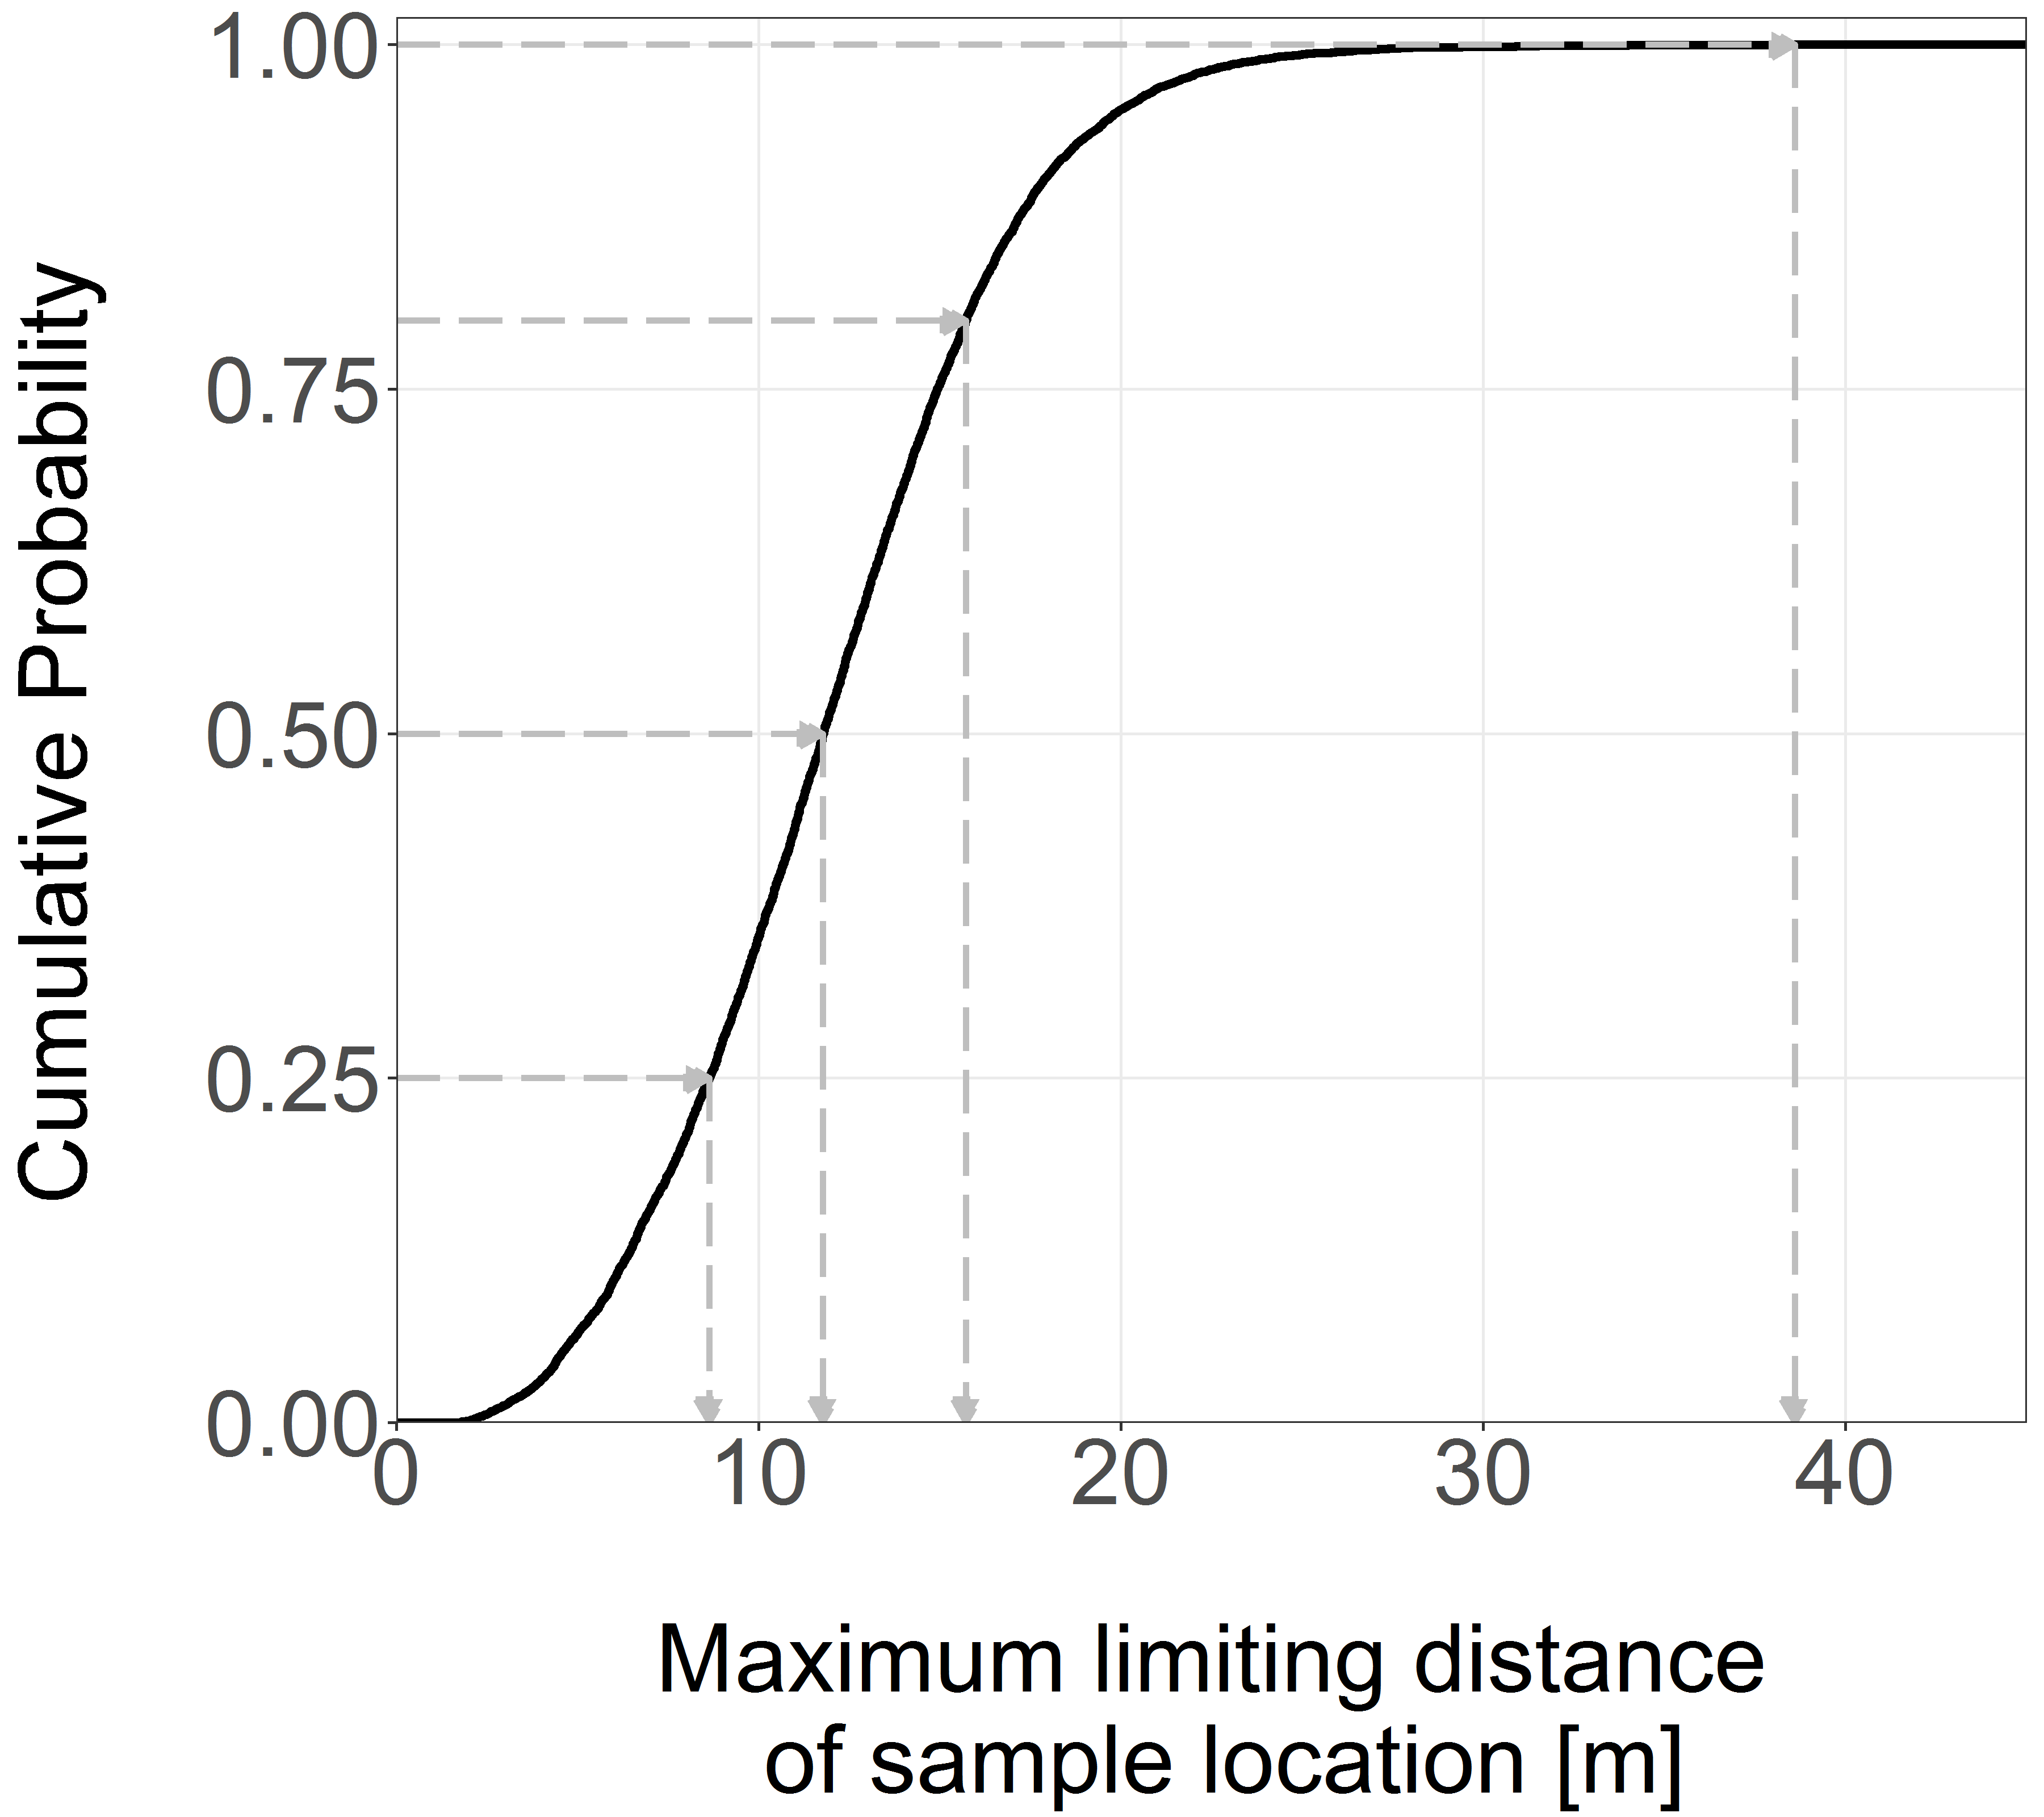
\includegraphics{Grafiken/Regmod_article/cdf_maxri.png}}%
		\caption{} \label{fig:sf1}
	\end{subfigure}
	\begin{subfigure}[t]{0.5\textwidth}
		\centering
		\resizebox{0.85\hsize}{!}{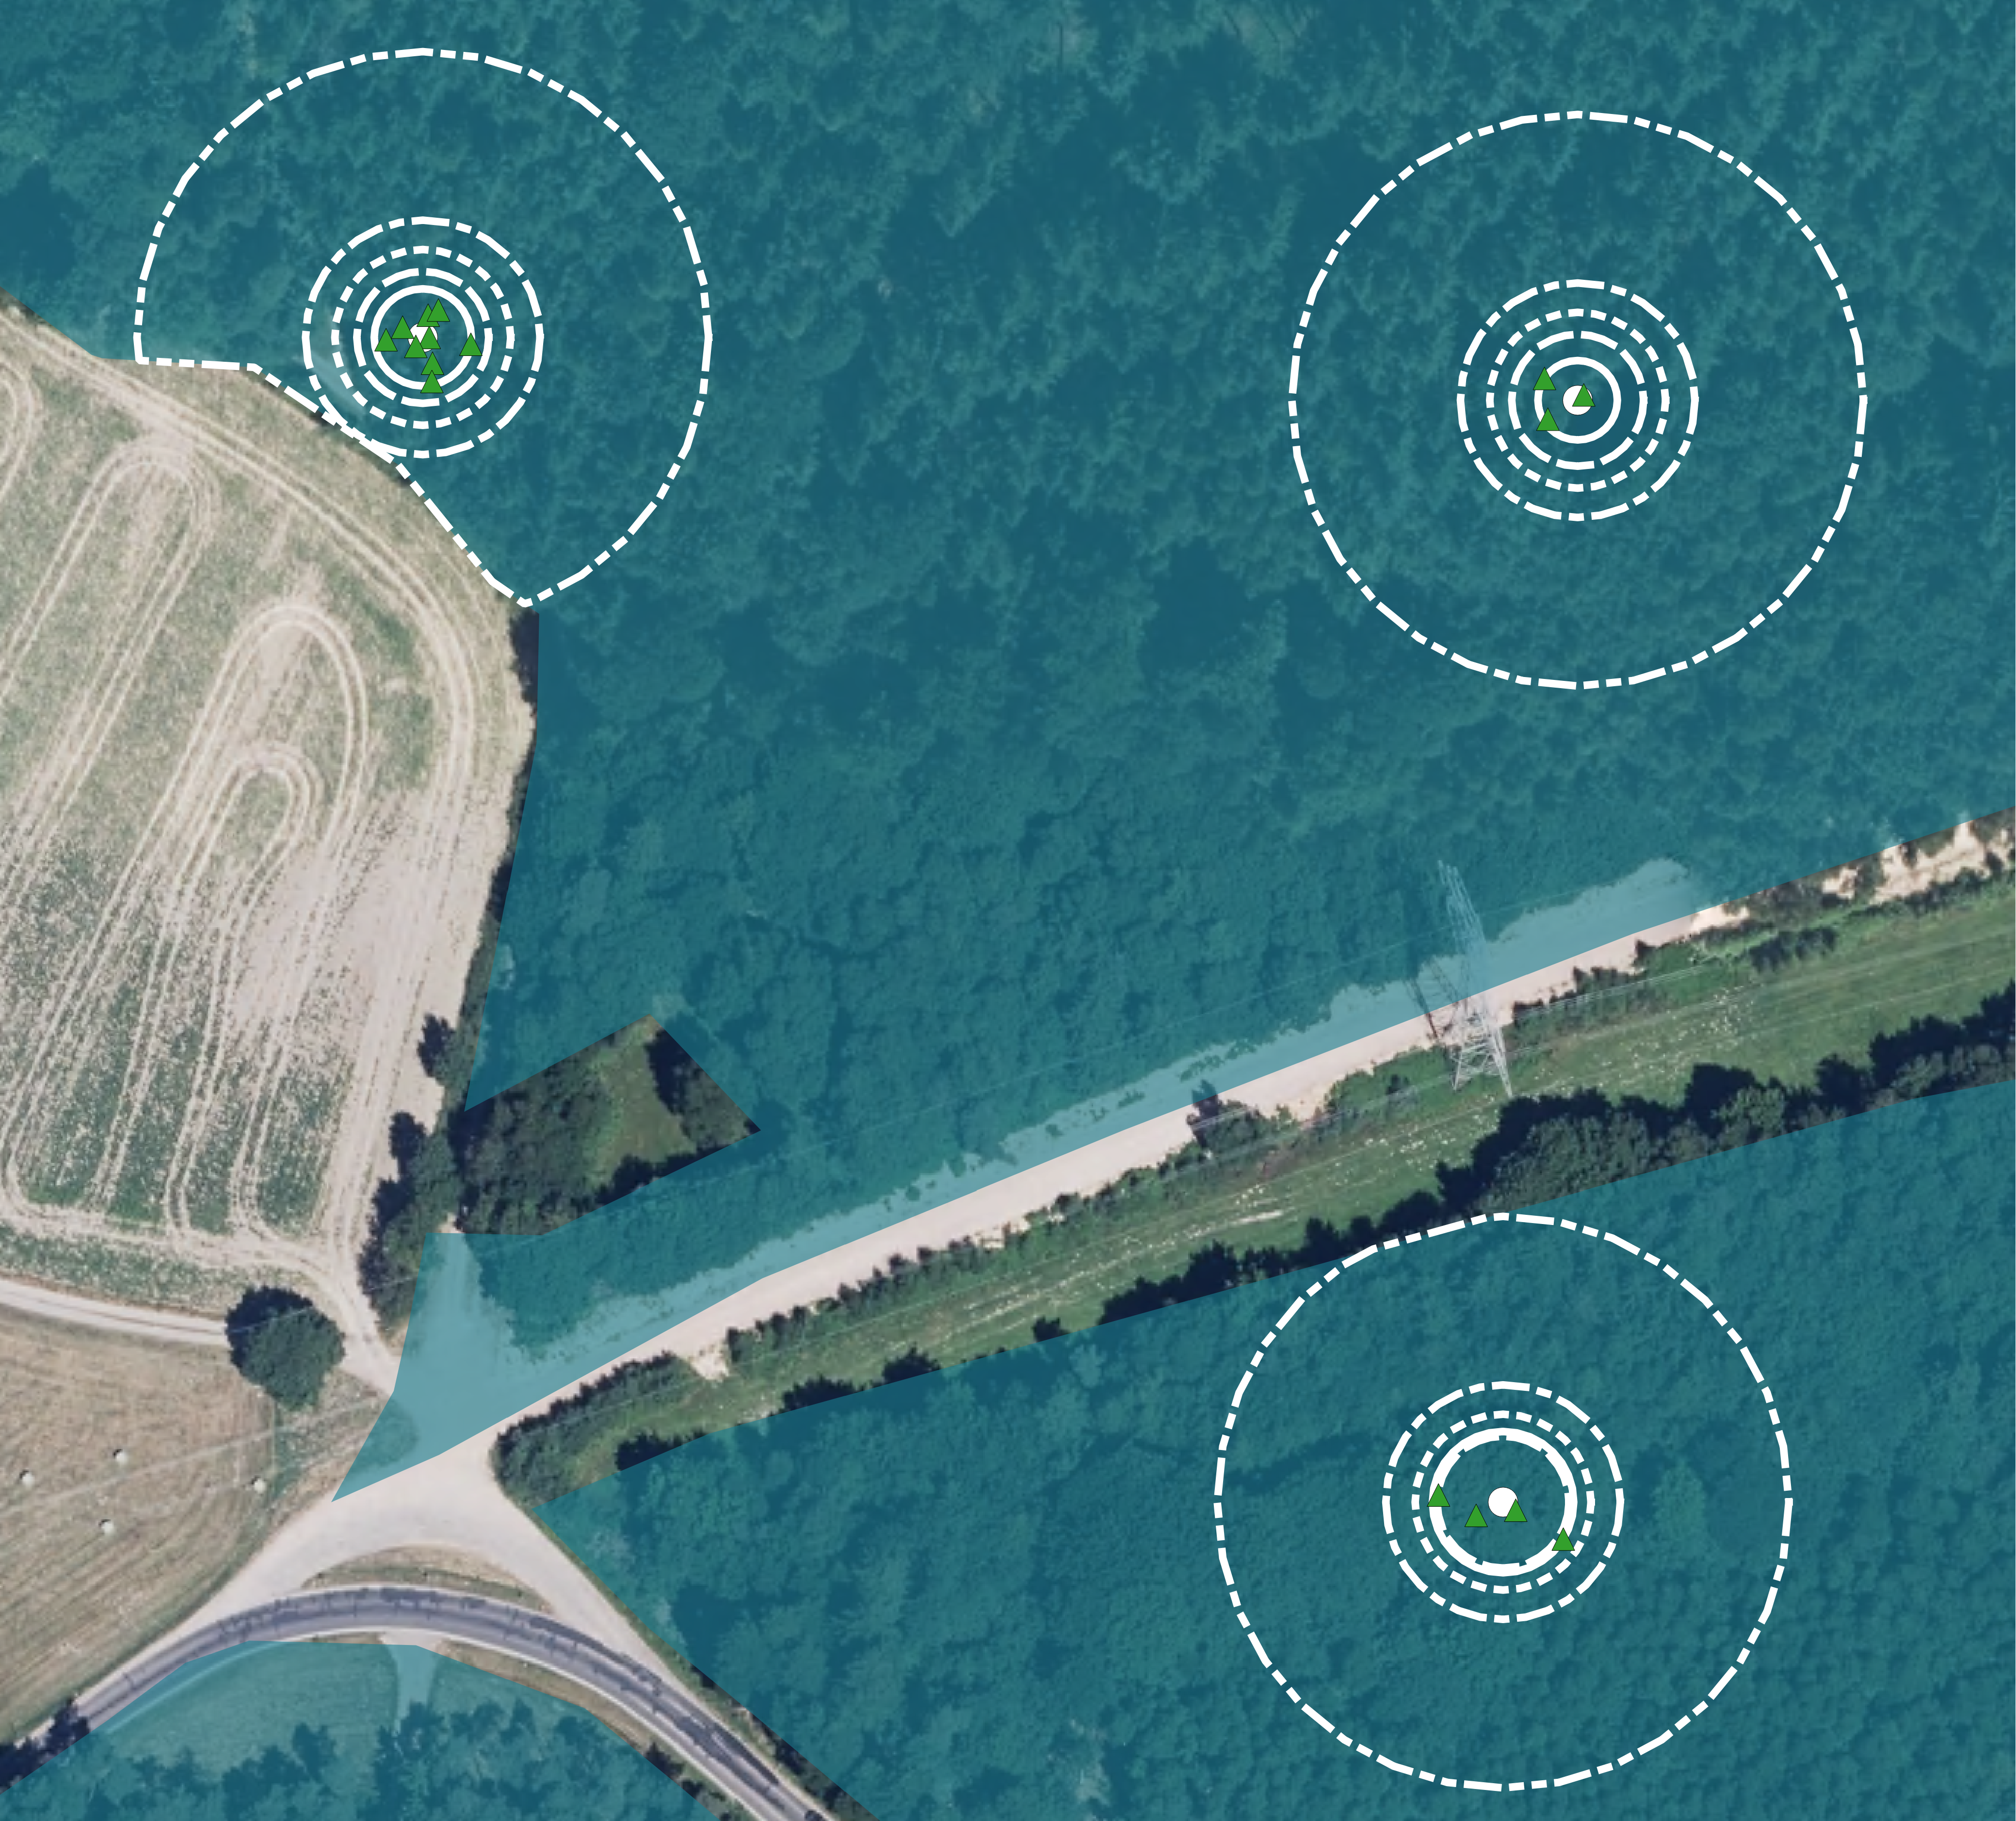
\includegraphics{Grafiken/Regmod_article/choice_of_support.png}}%
		\caption{} \label{fig:sf2}
	\end{subfigure}
     \caption{Identification (\textit{a}) and visualization (\textit{b}) of potential support radii used for calculating the predictor variables on plot level based on ECDF of maximum limiting distances of all \bwi{} sample locations in RLP.}
      \label{fig:tspec_supps}
\end{figure}

% ----------------------------------------------------------------------- %
% ----------------------------------------------------------------------- %
\subsection{\changed{Model Building and Evaluation}}
\label{sec:modval}

\changed{In order to judge the quality of the \textit{treespecies} variable, the user's accuracy for each classified species category and the overall accuracy of the classification scheme was calculated based on the confusion matrix \citep{congalton2008}. As reference data, we calculated the actual main plot tree species by applying the respective threshold to the sample trees of each sample plot.} The classification accuracy was evaluated for all support sizes for both the calibrated and the uncalibrated \textit{treespecies} variables. The measures of the regression model accuracy using both CHM- and $treespecies$ variables were defined as the 10-fold cross-validated root mean square error (\rmsecv{}, equation \ref{eq:RMSE}) and the adjusted coefficient of determination (\adjrsq{}) of the multiple linear regression model defined in equation \ref{eq:chmtspec_fullmod_term}. Additionally, we considered the interaction terms \textit{meanheight}:\textit{treespecies}, \textit{meanheight$^{2}$:treespecies}, \textit{meanheight}:\textit{ALSyear}, \textit{stddev}:\textit{ALSyear} and \textit{meanheight}:\textit{stddev} and performed a variable selection based on the Akaike Information Criterion (AIC) \citep{Akaike2011} in order to minimize the number of variables in the model. Due to a pronounced unbalanced design in the \textit{treespecies}-\textit{ALSyear} strata (Online Resource 2), no interaction between \textit{treespecies} and \textit{ALSyear} was possible. We evaluated the model for all support combinations, considering the use of individual support sizes for each auxiliary information, using both the calibrated and the uncalibrated \textit{treespecies} variable. The calibration model (section \ref{sec:tspecclass}) for the \textit{treespecies} variable was recalculated for each respective support-threshold setting.\par

206 sample plots included no sample trees and the timber volume density $Y(x)$ was thus set to \textit{zero}. These \textit{zero-plots} were removed from the modeling dataset since they acted as leverage points in cases where the ALS height metrics were recorded long before the terrestrial survey. Together with the missing tree species information (section \ref{sec:tspecclass}), the modeling dataset $s$ was limited to $n$=\changed{5171} observations.

\begin{subequations}\label{eq:RMSE}
	\begin{align}
	RMSE &= \sqrt{\frac{\sum_{x \in s}\big(\hat{Y}(x)-Y(x)\big)^2}{n}} \label{eq:RMSEa}\\
	RMSE\% &= \frac{RMSE}{\frac{1}{n}\sum_{x \in s}Y(x)}	\label{eq:RMSEb}
	\end{align}
\end{subequations}


\begin{equation} \label{eq:chmtspec_fullmod_term}
\begin{split}
Y(x) = &\beta_{0} + \beta_{1}*meanheight + \beta_{2}*meanheight^{2} + \beta_{3}*stddev + \\
&\beta_{4}*ALSyear_1 + ... + \beta_{12}*ALSyear_9 + \\
&\beta_{13}*treespecies_1 + ... + \beta_{18}*treespecies_6 + \varepsilon(x)
\end{split}
\end{equation}



%-------------------------------------------------------------------------------------------%
% ---------------------------------- Results ---------------------------------------------- %

\section{Results}
\label{sec:Res}

% ----------------------------------------------------------------------- %
% ----------------------------------------------------------------------- %
\subsection{Classification Accuracies}
\label{sec:supp_tspec_res}

\subsubsection*{Effect of Support Size and Threshold}

\changed{The lowest user's accuracies ($UA$) for the uncalibrated tree species variable were mostly realized using high thresholds of 80\% and 100\% (figure \ref{fig:cos_oaa_ua}).} A plausible reason for this is that raising the threshold to higher values (e.g. 80\%, 100\%) distinctively increases the probability of the reference class (based on the sample trees of the sample location) to be assigned as class 'Mixed', while the much coarser spatial resolution of the tree species map causes the $predicted$ class to remain classified as one of the five tree species. However, as the support size is  increased, so does the number of tree species raster cells to be evaluated at the sample location, thereby increasing the probability that the predicted class will be 'Mixed'. For this reason, most tree species exhibit an increase in user's accuracy under higher thresholds with higher support sizes. This scale-threshold dependency of the user's accuracy particularly affects tree species that most commonly occur in mixed forest stands in Rhineland-Palatinate (\textit{Scots pine}, $oak$ and $beech$), whereas the user's accuracies for tree species that are mostly prominent in pure forest stands ($spruce$, \textit{Douglas fir}) logically turned out to be much more robust to changes in the thresholds and support sizes.\par
Among the uncalibrated tree species predictions, $beech$ and $spruce$ produced the best predictions achieving UAs of up to 70\% and 80\%.  Although the predictions for \textit{Douglas fir} and \textit{Scots pine} generally performed less well than $beech$ and $spruce$, similar UAs can be produced by adjusting the threshold and support choices. UAs for $oak$ never performed better than 50\%. A detailed table of the user's and overall accuracies is provided in Online Resource 3.

\begin{figure}[H]
	\centering
	\resizebox{0.44\hsize}{!}{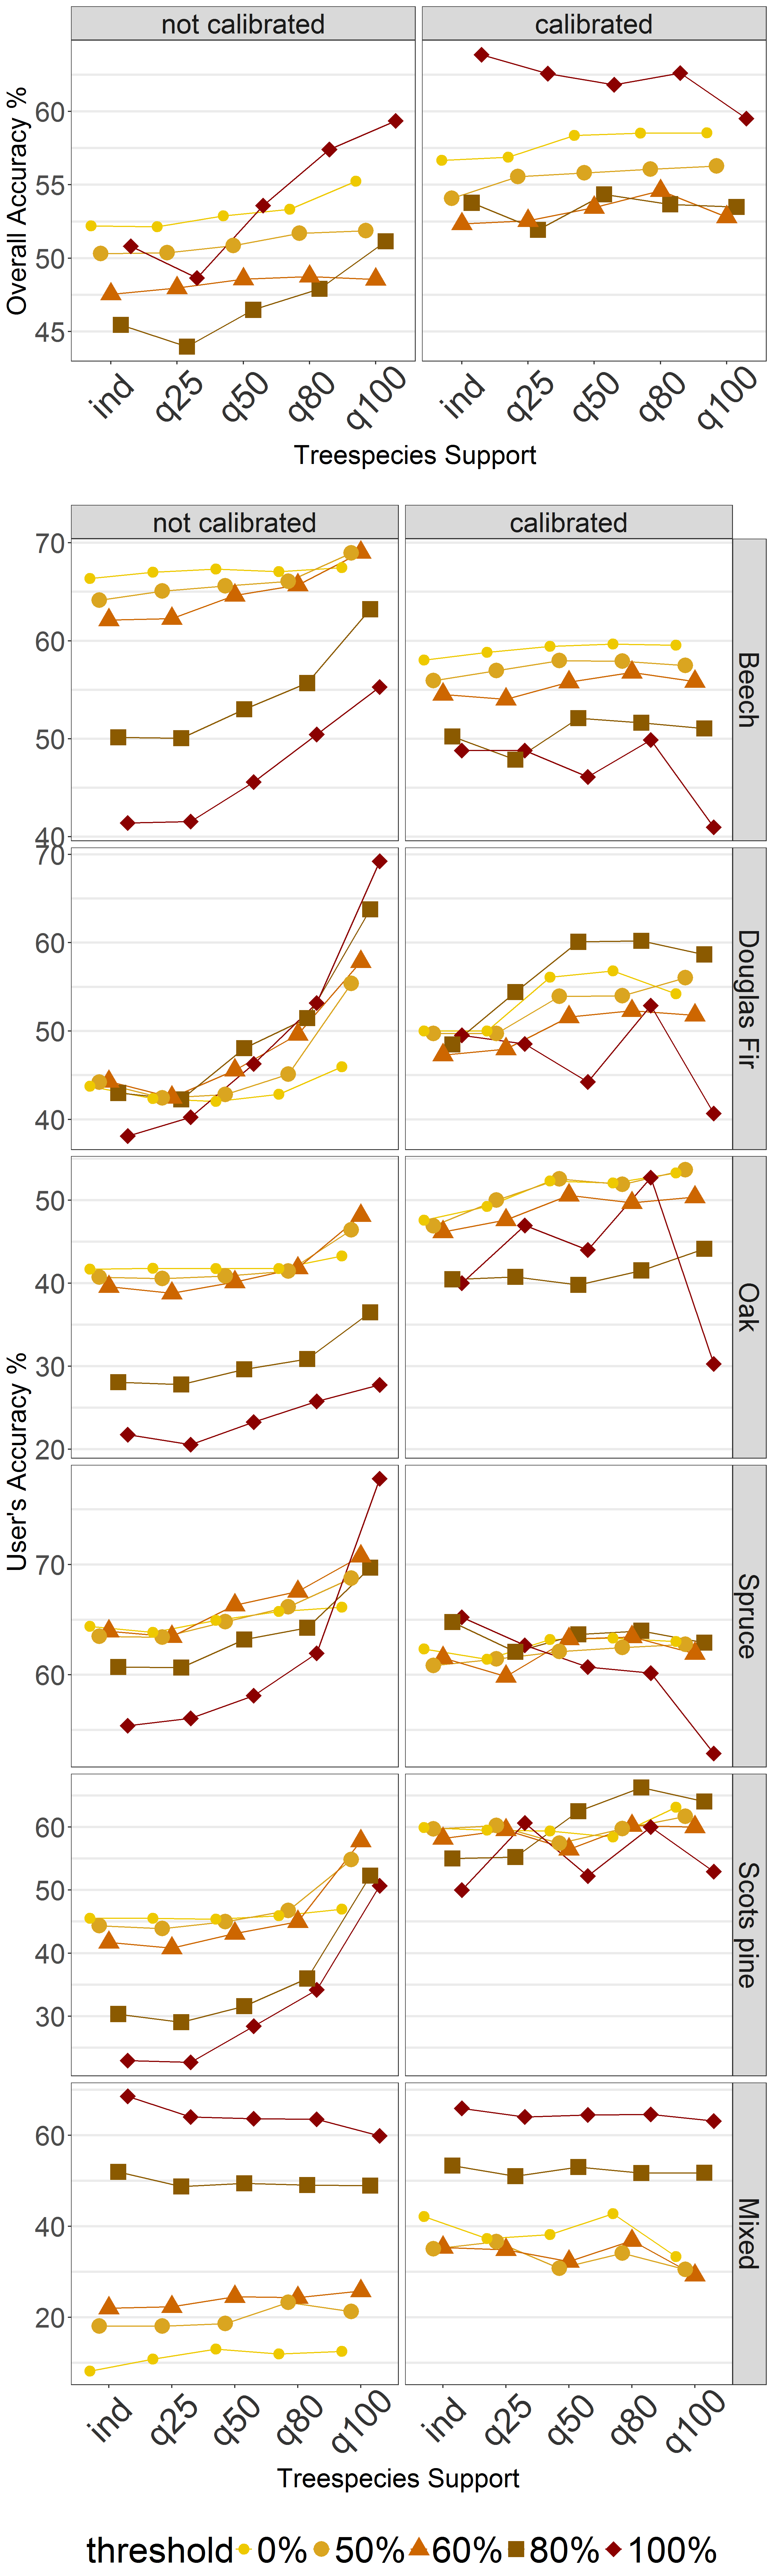
\includegraphics{Grafiken/Regmod_article/oaa_and_cos_tspec_mixed_cal_nocal.png}}
	\caption{Classification accuracy for the main tree species of a sample location \textit{before} and \textit{after} calibration: \textit{top)} overall accuracies. \textit{bottom)} user's accuracies. \textit{ind}: plot individual support sizes.}
	\label{fig:cos_oaa_ua}
\end{figure}


\subsubsection*{\changed{Calibration}}
Calibration substantially diminished the effect of the scale-threshold dependency for the five tree species and also increased the UAs for \textit{Scots pine} and $oak$. \changed{Whereas the UAs for $beech$ and $spruce$ were found to be slightly lower after calibration,} the overall accuracy under each support choice was always considerably increased by calibrating the tree species prediction (figure \ref{fig:cos_oaa_ua}). With respect to the calculated random forest models, the initial tree species prediction ($treespecies$) and the information about the growing region ($wgb$) turned out to be the most valuable information, followed by the estimated proportion of coniferous trees ($prop.conif$) and the mean canopy height ($meanheight$).


% ----------------------------------------------------------------------- %
% ----------------------------------------------------------------------- %
\subsection{Regression Model Accuracies}
\label{sec:supp_chm_tspec_res}


\subsubsection*{Effect of Support Size and Threshold}

Figure \ref{fig:supp_perf_res} shows the accuracies of the regression model (equation \ref{eq:chmtspec_fullmod_term}) achieved under all possible combinations of support sizes for the auxiliary data. The stepwise selection procedure always included all considered single and interaction terms. In terms of \adjrsq{} and \rmsecv{}, the analysis revealed that the choice of the CHM support size controls the overall level of the model's accuracy. The information about the main plot tree species can then be used to further improve the model fit under suitable $treespecies$ support and threshold settings. When using the uncalibrated $treespecies$ variable, an increase of the $treespecies$ support size causes an increase in the model performance if low thresholds are used, whereas high thresholds (80\%, 100\%) cause a decrease in the model performance. This threshold-dependency could be removed by calibrating the $treespecies$ variable. \changed{The highest \adjrsq{} and the lowest \rmsecv{} were realized using the $q50$ support for both the CHM and calibrated $treespecies$ variables in combination with a $treespecies$ threshold of 100\%, resulting in (\adjrsq{} of 0.48 and \rmsecv{} of 136.62 m$^2$/ha (43.8\%).} However, various support and threshold combinations for the CHM and $treespecies$ variables can be used to yield almost identical \rmsecv{} and \adjrsq{} values. A detailed table of the model accuracies is given in Online Resource 4.

\subsubsection*{Effect of Misclassifications}

\changed{We accessed the magnitude of the misclassification effect for all models that were analysed in section \ref{sec:supp_chm_tspec_res}, i.e. for all possible support and threshold combinations for the CHM and $treespecies$ predictor variables. We first compared the \adjrsq{} of each model when using the uncalibrated $treespecies$ variable against the \adjrsq{} using the actual, i.e. error-free variable. We then did the same comparison for the model using the calibrated treespecies predictor variable. Figure \ref{fig:supp_r2_calnocal} provides a visualization of this comparison. Note that only the model with the predicted tree species variables can be applied to additional sample locations where no terrestrial survey has been carried out.}\\
As expected, the highest \adjrsq{} for every evaluated model was always achieved using the error-free tree species variable, whereas the missclassifications in the tree species variable led to a systematic decrease of the model accuracy. The calibration of the initially predicted main plot tree species using the random forest classification algorithm (section \ref{sec:tspecclass}) turned out to not only improve the classification accuracies (section \ref{sec:supp_tspec_res}), but also to considerably decrease the effect of the missclassifications on the regression model predictions and accuracy. Figure \ref{fig:supp_r2_calnocal} ($right$) shows that the \adjrsq{} under the actual and the calibrated predicted tree species variable are in general much closer to, and in many cases even on the identity line. \added{The differentiation into two distinct point clouds results from the poor model performance under support size $q100$ for the CHM variables (i.e. the lower point cloud).} Whereas the misclassifications in the uncalibrated $treespecies$ variable led to a residual inflation of \changed{0.01 - 0.05} in \adjrsq{}, it was only between \changed{0 and 0.01} after calibration. Further analysis revealed that when using the calibrated $treespecies$ variable, the regression coefficients were almost identical to the ones received using the actual main plot tree species.

\begin{figure}[h]
	\centering
	\resizebox{1\hsize}{!}{\includegraphics*{Grafiken/Regmod_article/cos_cal_nocal_bw.png}}
	\caption{10-fold \rmsecv{}[\%] and \adjrsq{} realized under various support choices for the CHM and $tree species$ explanatory variables}
	\label{fig:supp_perf_res}
\end{figure}


\begin{figure}[h]
	\centering
	\resizebox{0.75\hsize}{!}{\includegraphics*{Grafiken/Regmod_article/cos_r2_cal_vs_nocal.png}}
	\caption{Effect on the \adjrsq{} when substituting the actual main tree species with the predicted  main tree species of a sample plot. The \textit{dotted} line tracks the the model with the highest \adjrsq{} under the use of the error-free \textit{treespecies} variable. Semitransparent colours for the data points are used to visualize overlap.}
	\label{fig:supp_r2_calnocal}
\end{figure}


% ----------------------------------------------------------------------- %
% ----------------------------------------------------------------------- %
\subsection{Final Regression Model}
\label{sec:regmod_final}

In order to address research questions 1 and 2 (i.e. the gain in model accuracy by tree species information and effect of heterogeneity in the ALS data), we investigated the model properties in more detail. For this purpose, we decided to use the best found model that was achieved under the support settings of $q50$ for both auxiliary data with a threshold of 100\% for the tree species variable as the regression model of choice. The reason for inspecting this model was that \textit{a)} the model provided the highest \adjrsq{} among all validated models while reducing the data handling complexity for upcoming applications (i.e. identical support sizes for all remote sensing data) and \textit{b)} the calibration neutralized the effects of misclassifications on the model predictions. The interaction term between $meanheight^2$ and $treespecies$ (i.e. considering separate curvatures for each tree species) turned out not to have a significant influence on the model accuracy and was dropped, resulting in an \adjrsq{} of 0.48 and a slightly increased \rmsecv{} of 140.62 m$^2$/ha (46.7\%). \added{The final model thus comprised 39 parameters (regression coefficients), i.e. the intercept, 3 main effects for continuous variables, 13 main effects for categorical variables and 22 interaction parameters (table \ref{tab:modacc_modterms}).\par
	We also conducted an analysis for detecting influential data points or outliers for the final regression model. We here considered the commonly applied criteria of leverages and Cook's Distance as amongst others described in \citet[p. 160-167]{fahrmeir2013}. The critical threshold of $2p/n$ (i.e. twice the average of the hat matrix' diagonal entries) was exceeded by 10\% of the observations. However, only 3\% of these leverage points were assigned to studentized residuals with values $>$ 1 or $<$ -1. Removing these observations from the dataset and refitting the model led to an \adjrsq{} of 0.49 compared to 0.48 when including them. Additionally, Cook's Distance values $D_i$ did not exceed a value of 0.019, and were thus far apart from the commonly used critical threshold of $D_i >$ 0.5 that indicate a considerably change of the regression model results when omitting them. We thus decided not to remove any observations from the modelling dataset. We thus decided not to remove any observations from the modelling dataset.}

\begin{figure}[h]
	\centering
	\resizebox{0.91\hsize}{!}{\includegraphics*{Grafiken/Regmod_article/predlines_tspecaux_cal.png}}
	\caption{Visualization of the timber volume prediction function (\textit{final regression model}) on sample plot level for each main plot tree species and ALS acquisition year. For visualization purposes, the predictor variable $stddev$ was set to its average value within the respective \textit{treespecies} and \textit{ALSyear} categories. The terrestrially observed timber volume values are plotted in the background.}
	\label{fig:predlines_tspec}
\end{figure}

% latex table generated in R 3.4.2 by xtable 1.8-2 package
% Sun Jan 07 17:11:26 2018
\begin{table*}[!htbp]
	\centering
	\caption{Accuracy specifications for submodels of final OLS regression model. $p$ gives the number of parameters for each model. Interaction terms are indicated by ':'.} 
	\label{tab:regmod:mt}
	\begin{tabular}{llrrrr}
  \hline
model terms & model & $p$ & $R^2_{adj}$ & $RMSE_{cv}$ & $RMSE_{cv}\%$ \\ 
  \hline
  meanheight + stddev + meanheight$^2$ + \\ treespecies + ALSyear + \\ meanheight:treespecies + \\ meanheight:ALSyear + meanheight:stddev \\ + stddev:ALSyear & Final model &  39 & 0.48 & 140.62 & 46.69 \\ \\
  meanheight + stddev + meanheight$^2$ + \\ meanheight:stddev & Submodel 1 &   5 & 0.36 & 155.54 & 51.65 \\ \\
  meanheight + stddev + meanheight$^2$ + \\ ALSyear + meanheight:ALSyear + \\ meanheight:stddev + stddev:ALSyear & Submodel 2 &  29 & 0.45 & 145.62 & 48.35 \\ \\
  meanheight + stddev + meanheight$^2$ + \\ treespecies + meanheight:treespecies + \\ meanheight:stddev & Submodel 3 &  15 & 0.40 & 150.32 & 49.92 \\ 
   \hline
\hline
\end{tabular}
\end{table*}
%\endgroup


%% old version
%\begin{table*}
%	\centering
%	\caption{Accuracy metrics for submodels of final OLS regression model} 
%	\label{tab:modacc_modterms}
%	\begin{tabular}{llrrr}
%		\hline
%		model terms & model & parameters & $R^2_{adj}$ & \rmsecv{} \\ 
%		\hline
%		meanheight + stddev + meanheight$^2$ + \\ treespecies + lidaryear + meanheight:treespecies + \\ meanheight:lidaryear + meanheight:stddev + \\ stddev:lidaryear & final model &  39 & 0.49 & 132.12 \\ \\
%		meanheight + stddev + meanheight$^2$ + \\ meanheight:stddev & submodel 1 &   5 & 0.35 & 148.03 \\ \\
%		meanheight + stddev + meanheight$^2$ + \\ lidaryear + meanheight:lidaryear + \\ meanheight:stddev + stddev:lidaryear & submodel 2 &  29 & 0.44 & 137.52 \\ \\
%		meanheight + stddev + meanheight$^2$ + \\ treespecies + meanheight:treespecies + \\ meanheight:stddev & submodel 3 &  15 & 0.41 & 137.52 \\ 
%		\hline
%		\hline
%	\end{tabular}
%\end{table*}
%%\endgroup

\subsubsection*{Interpretation of Final Regression Model}
\label{sec:prop_regmod_final}
Figure \ref{fig:predlines_tspec} provides a visualisation of the tree species prediction functions separated by the ALS acquisition years. Sample plots classified as $oak$ and \textit{Scots pine} revealed to have an almost identical relationship (nearly identical slopes) for the mean canopy height - timber volume relationship. They only differ by a marginally higher intercept for \textit{Scots pine} plots, meaning that given the same mean canopy height a sample plot dominated by \textit{Scots pine} yields a marginally higher timber volume on the plot level than a plot dominated by $oak$. $Beech$-dominated sample plots tend to achieve a higher timber volume than $oak$ and \textit{Scots pine} for canopy heights below 20 meters, but realize the lowest timber volumes for canopy heights above 20 metres. Sample plots dominated by any of the remaining coniferous tree species (\textit{Douglas fir}, $spruce$) revealed to have higher slopes than broadleaf classified plots. This indicates that given the same mean canopy height, sample plots dominated by \textit{Douglas fir} and $spruce$ yield higher timber volume values than broadleaf- or \textit{Scots pine} dominated sample plots, and this difference becomes more pronounced with increasing mean canopy heights. Within the group of coniferous-dominated sample plots, $spruce$ turned out to have the highest slope, thereby yielding the highest timber volume values for mean canopy heights above 15 meters. An undesired characteristic of the model is that the predicted timber volume can in some cases ($<$ 1\%) take negative values for low canopy heights (e.g. for $spruce$-dominated plots with \textit{meanheight} below 5 meters and $stddev$ of 4 meters). \changed{However, we chose not to use a log-transformation of the response variable. Doing so would have prevented the subsequent calculation of the g-weight variance of the design-based estimators \citep{mandallaz2013a, mandallaz2013b}, which is only possible for response variables on the original scale. The g-weight variance provides the benefit of a better variance estimate for internal models by considering the dependency of the regression coefficients on the realized sample. The rare occurrence of negative predictions were however not considered to have an influence on subsequent design-based estimates when averaging multiple predictions within given spatial domains.}


\subsubsection*{Effect of Time-Lags and Heterogeneity in ALS Data}

Incorporating the ALS acquisition year as a categorical variable ($ALSyear$) in the regression model substantially accounted for the variability in the data introduced by \textit{a)} the time-lags between ALS acquisition and terrestrial survey, and \textit{b)} variation in ALS data quality which are due to sensor- and post processing techniques (table \ref{tab:modacc_modterms}). \changed{Whereas the \adjrsq{} for the regression model without considering the ALS acquisition year as additional predictor variable (\textit{submodel 1}) was 0.36, it could already been increased to 0.40 by including the tree species variable (\textit{submodel 2}). A further stratification by the ALS acquisition year increased the \adjrsq{} of \textit{submodel 1} from 0.36 to 0.45, and the \adjrsq{} of \textit{submodel 3} from 0.40 to 0.48.}\par

We further analysed the model residuals within each ALS acquisition year (within-group variation) for the final model and nested submodels. It turned out that the $R^2$ values vary distinctly between the ALS acquisition year strata (table \ref{tab:adj_r2_within}). More precisely, the within-group $R^2$ can be higher and lower than the overall $R^2$ of the respective model. Figure \ref{fig:r2adj_in_lyears} shows that a stratification according to the ALS acquisition years (submodel 2) can already increase the $R^2$ in most acquisition year strata, compared to the basic model using only the ALS height metrics as predictor variables (submodel 1). In the ALS acquisition year stratum 2007, the increase in $R^2$ even reached 0.08.

% latex table generated in R 3.4.2 by xtable 1.8-2 package
% Sun Jan 07 17:26:28 2018
\begin{table}[ht]
	\centering
	\caption{$R^2$, RMSE and RMSE\% of final regression model within ALS acquisition year strata (\textit{ALSyear}). $Area_{ALSyear}$: Area covered by ALS acquisition given in km$^2$. \textit{n}: number of validation data.}
	\label{tab:regmod:adj_r2_within}
	\begin{tabular}{lllrrr}
		\hline
		\textit{ALSyear} & $Area_{ALSyear}$ & $R^2$ & RMSE & RMSE\% & n \\ 
		\hline
 2012 & 2807   & 0.61 & 135.84 & 44.87 & 408 \\ 
 2011 & 4361  & 0.57 & 146.21 & 48.29 & 883 \\ 
 2010 & 4182 & 0.51 & 120.90 & 39.93 & 1171 \\ 
 2009 & 2100 & 0.42 & 133.42 & 44.07 & 559 \\ 
 2008 & 2968 & 0.48 & 130.38 & 43.06 & 701 \\ 
 2008\_1 & 2116 & 0.33 & 175.43 & 57.94 & 394 \\ 
 2007 & 3498 & 0.46 & 136.47 & 45.08 & 418 \\ 
 2003 & 602 & 0.27 & 154.48 & 51.02 & 529 \\ 
 2002 & 775 & 0.44 & 141.55 & 46.75 & 314 \\ 
		\hline
\hline
\end{tabular}
\end{table}
%\end{longtable}
%\endgroup

%% old version
%\begin{table}[ht]
%	\centering
%	\caption{$R^2$, RMSE and Residual Square Sum (SSE) of final regression model within LiDAR acquisition year strata (\textit{lidaryear}). \textit{n}: number of validation data}
%	\label{tab:adj_r2_within}
%	\begin{tabular}{llrrr}
%		\hline
%		LiDAR acquisition year & $R^2$ & rmse & SSE & n \\ 
%		\hline
%		2012   & 0.55 & 139.54 & 7535278 & 387 \\ 
%		2011   & 0.55 & 145.21 & 17880553 & 848 \\ 
%		2010   & 0.48 & 122.16 & 16907662 & 1133 \\ 
%		2009   & 0.43 & 127.17 & 8652419 & 535 \\ 
%		2008\_1 & 0.34 & 170.49 & 11161424 & 384 \\ 
%		2008   & 0.50 & 124.39 & 10475374 & 677 \\ 
%		2007   & 0.49 & 129.72 & 6950192 & 413 \\ 
%		2003   & 0.32 & 146.37 & 11139814 & 520 \\ 
%		2002   & 0.43 & 139.79 & 6038601 & 309 \\ 
%		\hline
%		\hline
%	\end{tabular}
%\end{table}
%%\end{longtable}
%%\endgroup


\begin{figure}[H]
	\centering
	\resizebox{0.62\hsize}{!}{\includegraphics*{Grafiken/Regmod_article/r2adj_in_lyears.png}}
	\caption{$R^2$-values of the final regression model, submodel 1 and submodel 2 achieved $within$ the ALS acquisition year strata.}
	\label{fig:r2adj_in_lyears}
\end{figure}


\subsubsection*{Added Value of Tree Species Map Information}
\changed{Introducing the predicted main tree species of a sample plot as an additional categorical variable to submodel 2 yielded a further increase in the \adjrsq{} of 0.03 (table \ref{tab:modacc_modterms}). However, the improvement was even more pronounced in ALS acquisition years close or identical to the year of the terrestrial inventory (figure \ref{fig:r2adj_in_lyears}). We observed an increase of 0.06 in $R^2$ for ALS acquisition year 2012, and of 0.07 for ALS acquisition year 2011.} The analysis illustrated once more that misclassifications in the tree species variable generally reduce model accuracy compared to using error-free tree species information. The residual inflations caused by the misclassifications in the uncalibrated $treespecies$ variable within the $ALSyear$ strata were up to 0.05 in R$^2$. However, the calibration was able to substantially decrease or even remove the effects of misclassifications on the model accuracy in all ALS acquisition year strata.


%----------------------------------------------------------------------------------------------%
% ---------------------------------- Dsicussion ---------------------------------------------- %

\section{Discussion}
\label{sec:Dis}

% ----------------------------------------------------------------------- %
% ----------------------------------------------------------------------- %
\subsection{Stratification according to ALS Acquisition Years and Tree Species}
\label{sec:strat_dis}

Incorporating the main tree species of a sample location in the timber volume regression model increased the model accuracy and revealed strong evidence for the existence of a tree species specific behavior concerning timber volume on the plot level. This result seems reasonable regarding the species specific taper functions on single-tree level applied in the \bwi{} \citep{kublin2003, kublin2013}. \added{
	These findings also agree with those of \citet{latifi2012} who found an almost identical improvement in RMSE of 2\% when stratifying to broadleaf and coniferous tree species. The overall RMSE of their model  was however 10\% smaller than in our study. This might be due to a more heterogeneous dataset of much smaller sample size, but also because the temporal alignment between the auxiliary data acquisition and the terrestrial survey was much better. Additionally, the number of different tree species present in their dataset was lower than in our case and only comprised Scots pine, European beech and oak. The individual effects of spruce and Douglas fir indicated by our model also support the findings of \citet{breidenbach2008}, who found a higher percentage of coniferous trees in a sample plot to increase the timber volume predictions. This was not true for Scots pine and oak whose effects turned out to be very similar for our dataset. However, in our study the stratification according to the ALS acquisition years severely limited the flexibility of species-specific prediction functions and model interpretability.} In particular, using the ALS acquisition years as categorical variables led to highly unbalanced datasets when stratifying according to the main plot tree species. This prevented the use of further stratification variables such as bioclimatic growing regions due to confounding effects and consequent singularities in the design matrices. \added{It also implied an artificial increase in the number of parameters in the OLS regression model, which was however not regarded as critical with respect to overfitting issues due to the high amount of observations used for fitting the regression coefficients \citep[Ch. 15.1]{draper2014}.} A stratification to the ALS acquisition years however proved to be an effective means in accounting for the artificially introduced noise in the data caused by quality variations and the large time-lags between the remote sensing and terrestrial data. \added{It allowed for a model accuracy that was very close to those reported by \citet{maack2016} who conducted a very similar study in the German federal state of Baden-W\"urttemberg.} Model accuracies were also particularly higher in ALS acquisition year strata in which the data showed considerably less noise or were closer to the date of the terrestrial survey. \added{This effect was significantly reduced or even removed when merging several ALS acquisition year strata. Promising steps with respect to more up-to-date canopy height information have already been made, as the topographic survey institution of RLP is currently processing a canopy height model from aerial imagery acquisitions for 2011 and 2012 covering the entire federal state. These aerial photography acquisitions will in the future be conducted in a two-year period, allowing to derive up-to-date canopy height information in the framework of future forest inventories. For a smaller study area, \citet{kirchhoefer2017} have already demonstrated that similar model accuracies for German NFI data can be achieved using imagery-based canopy height models.}\par

Incorporating the calibrated tree species information further improved the model accuracy by \changed{0.03} in adjusted R$^2$. Compared to the simple model only containing ALS height metrics, including the ALS quality and calibrated tree species information increased the adjusted $R^2$ by \changed{0.12} in total. A differentiated evaluation of the final regression model revealed that the highest R$^2$-values were achieved within ALS acquisitions year strata close or identical with the year of the terrestrial survey, showing differences of up to \changed{0.3} between the R$^2$s. Also the gain in R$^2$ by including the tree species information was largest (i.e. \changed{0.07}) in combination with ALS information acquired in the year of the terrestrial inventory. These insights were particularly interesting with respect to the further use of the regression model for small area estimations. Small area estimators generally gain modeling strength by defining the prediction model $globally$ (i.e. using all data in the inventory area), and then applying the so-derived prediction model to a subset of observations located within the area of interest \citep{mandallaz2013a}. Consequently, the proposed stratification technique in the prediction model is expected to yield a gain in model accuracy and a reduction of the small area estimation errors if the small area domain mostly includes data from strata that have high within-strata model accuracies. \added{Findings of \citet{breidenbach2008} indicated that a further increase in model accuracies could possibly be achieved when incorporating these categorical variables as random rather than fixed-effects in linear mixed-effects models \citep{pinheirobates2000}. The reason we did not apply this family of models was that small area regression estimators subsequently applied in RLP \citep{mandallaz2013a, mandallaz2013b} require the internal models to be fitted by OLS technique.}\par


% ----------------------------------------------------------------------- %
% ----------------------------------------------------------------------- %
\subsection{Calibration of Tree Species Map Information}
\label{sec:calib_dis}
The accuracy assessment of the initially derived main plot species from the classification map revealed the presence of misclassifications that led to a decrease in model accuracy. \added{This is in agreement with the potential effects of erroneous explanatory variables discussed in \citet{carroll2006} and \citet{gustafson2003}, i.e. an increase of variability (noise) in the data that can increase the amount of unexplainable variance and thereby reduce the model accuracy.} One reason for the misclassifications were that the classification algorithm of \citet{stoffels2015} was exclusively trained in pure stands with the objective to predict the \textit{dominant tree species} of a forest stand. Thus, our requirements on the classification map differed considerably from the ones imposed by \citet{stoffels2015} and have to be considered as far more difficult to meet. Firstly, the reference data used in the accuracy assessment also included understory trees that were recorded in the \bwi{} sample. Secondly, determining an exact spatial validation unit for a sample location (support) is not possible due to the properties of angle count sampling (section \ref{sec:supp}). Thirdly, distinct discrepancies in the spatial scale between the reference data and the classification map severely hamper exact predictions of the main plot tree species especially in mixed forest stands. The latter issue caused a pronounced dependency of the user's accuracy on the support and threshold choice, particularly for tree species that most commonly occur in mixed forest structures, i.e. \textit{Scots pine} (91\%), $oak$ (90\%) and $beech$ (85\%) \citep{bwi3}. With respect to this set-up, the application of our calibration method proved to be of high value. It led to an increase in the classification accuracies, particularly for those tree species that performed worse in the uncalibrated setup, and thereby successfully minimized and even removed the deleterious effect of misclassifications on model accuracy and regression coefficients. Whereas the extensive analysis in our study deepened the understanding of the afore mentioned scale-effects, an alternative method for future applications could be to use map-derived percentages of each tree species as predictor variables in the random forest algorithm in order to directly predict the terrestrially observed main plot tree species.


% ----------------------------------------------------------------------- %
% ----------------------------------------------------------------------- %
\subsection{Choice of Support under Angle Count Sampling}
\label{sec:supp_choice_dis}

\changed{The validation of different support sizes underlined that the support choice can impact the accuracy of a prediction model, and thus confirmed the findings of \citet{deo2016}. In the present study, differences in the model accuracies however turned out to be small for most support choices. An exception was the choice of the $q100$ support for the CHM derived variables (76 meter radius), where the model accuracy was considerably worse than under the optimal settings. Contrary to our hypothesis, the use of plot-individual supports did not yield the best prediction performance overall. \citet{kirchhoefer2017} recently came to the same result when they transferred the angle-count sampling technique to a pixel-wise selection method of the auxiliary data that resembles the sample tree selection even more precisely. In their study, the application of fixed support sizes did also not perform worse than under variable supports. We consider two plausible reasons for the joint findings: first, the determination of an exact spatial extent that can be transferred to auxiliary data extraction remains technically infeasible under angle count sampling. Thus, angle count sampling does not seem to be adequate when linking inventory information with remote sensing data. Secondly, inaccuracies in the DGPS-measurements of the plot center locations as reported by \citet{lambrecht2017} may have an increased impact on the model accuracy the more exact the auxiliary data derivation spatially corresponds to those of the field survey. However, the extensive analysis carried out in our study also indicated that the optimal support size does not only depend on the spatial extent of the field plots, but also on the spatial resolution of the remote sensing data as well as the context in which the derived information is used in the prediction model. In the case of transforming the tree species information map into a suitable categorical predictor variable, the use of a large support size of 76 meter radius turned out to yield the best model accuracy. However, only few sample locations in the study area were actually characterized by limiting circles of that particular size. An analysis to find the best support settings therefore seems to be advisable prior to further applications of design-based or model-dependent inventory methods so as not to lose model accuracy by unsuitable support choices. The concept of the demonstrated analysis method for identifying suitable supports can be transferred to any kind of auxiliary information, predictor variable and prediction model.}


%----------------------------------------------------------------------------------------------%
% ---------------------------------- Conclusion ---------------------------------------------- %

\section{Conclusion}
\label{sec:concl}

\changed{We draw three major conclusions from our study: (1) our analyses strongly indicated that the acquisition of auxiliary data close to the date of the terrestrial survey is a key factor to achieve good model accuracies. Particularly for large-scale inventory applications, this requirement is often difficult to meet. In such cases, we consider that the proposed method of including quality information about the auxiliary data in a prediction model can be an effective technique for improving the prediction accuracy. Ongoing studies investigate whether this modelling technique can also lead to smaller estimation errors of design-based estimators. (2) Our study also indicated that the relationship between the field measured timber volume and remote-sensing derived height information is tree species specific. We expect that using the tree species information in a timber volume model would even lead to higher prediction accuracies when combined with explanatory variables that can further explain the variation within each tree species group, such as bioclimatic growing conditions, soil properties and stand density on the plot level. (3) We consider the demonstrated calibration technique to be a valuable method for future studies where an external tree species map (i.e. the map was not created for the specific study objective) is used in prediction models. The application of a calibration model can also be transferred to any error-prone explanatory variable and be a simple means to clean the data set from noise and thus increase the model accuracy.}\\

%------------------------------------------------------------------------------------------------%
% ---------------------------------------- Acknowledgements ------------------------------------ %

%\section*{Acknowledgements}
%
%We want to express our gratitude to Prof. H. Heinimann (Chair of Land Use Engineering, ETH Zurich) for supporting this study. We want to explicitly thank Dr. Johannes Stoffels from the Environmental Sensing and Geoinformatics Group of Trier University for providing the tree species classification map as well as for constructive discussions when it came to interpreting the results. Special gratitude is owed to the State Forest Service of Rhineland-Palatinate, in particular Dr. Joachim Langshausen, J{\"u}rgen Dietz and Claus-Andreas Lessander, for collaboration and providing the forest inventory and geodata. We also want to thank Kai Husmann and Christoph Fischer from the Northwest German Forest Research Institution G{\"o}ttingen for their advice in processing the terrestrial inventory data, and Alexander Massey and Michael Hill for proofreading.









	\clearpage
	\newpage
	\mbox{}
	\pagebreak
	\thispagestyle{empty}

%%% ------------------------------ Artikel Small Area Estimation -------------------------------------- %%
\chapter{A double-sampling extension of the German National Forest Inventory for design-based small area estimation of timber volume resources on forest district levels}
\label{chap:regmod}
{\large Andreas Hill$^1$, Daniel Mandallaz$^1$, Joachim Langshausen$^2$}\\

\vspace{3cm}
\noindent
$^1$ETH Z\"urich\\Department of Environmental Systems Science, Universit\"atstrasse 16, 8092 Z\"urich, Switzerland \\

\vspace{\fill}
\noindent
In progress

\newpage
\renewcommand{\labelitemi}{--}
\begin{itemize}
	\item Daniel Mandallaz developed the design-based estimators. He also supported the statistical analysis and writing of the manuscript.
	\item Joachim Langshausen supported writing of the manuscript.
\end{itemize}

\clearpage
\clearpage
\newpage
\mbox{}
\pagebreak
\thispagestyle{empty}
	
%%% ------------------------------ Artikel 4 Mapping -------------------------------------------------- %%
\chapter{Accuracy assessment of timber volume maps using forest inventory data and LiDAR canopy height models}
\label{chap:mapp}
{\large Andreas Hill$^1$, Jochen Breschan$^1$, Daniel Mandallaz$^1$}\\

\vspace{3cm}
\noindent
$^1$ETH Z\"urich\\Department of Environmental Systems Science, Universit\"atstrasse 16, 8092 Z\"urich, Switzerland \\

\vspace{\fill}
\noindent
Published in:\\
\textit{Forests} 5 (2014): 2253-2275\\
(DOI: 10.3390/f5092253)

\newpage
\thispagestyle{plain}
\renewcommand{\labelitemi}{--}
\begin{itemize}
	\item Jochen Breschan supported the formulation of the optimization model.
	\item Daniel Mandallaz supported the statistical data analysis.
\end{itemize}

\clearpage

\clearpage
%%%%%%%%%%%%%%
%% Abstract %%
%%%%%%%%%%%%%%
\section*{Abstract}
\label{chap:regmod:Abstract}

Maps of standing timber volume provide valuable decision support for forest managers and have therefore been the subject of recent studies. For map production, field observations are commonly combined with area-wide remote sensing data in order to formulate prediction models, which are then applied over the entire inventory area. The accuracy of such maps has frequently been described by parameters such as the root mean square error of the prediction model. The aim of this study was to additionally address the accuracy of timber volume classes, which are used to better represent the map predictions. However, the use of constant class intervals neglects the possibility that the precision of the underlying prediction model may not be constant across the entire volume range, resulting in pronounced gradients between class accuracies. This study proposes an optimization technique that automatically identifies a classification scheme which accounts for the properties of the underlying model and the implied properties of the remote sensing support information. We demonstrate the approach in a mountainous study site in Eastern Switzerland covering a forest area of 2000 hectares using a multiple linear regression model approach. A LiDAR-based canopy height model (CHM) provided the auxiliary information; timber volume observations from the latest forest inventory were used for model calibration and map validation. The coefficient of determination (R$^2$ = 0.64) and the cross-validated root mean square error (\rmsecv{} = 123.79 m$^3$/ha) were only slightly smaller than those of studies in less steep and heterogeneous landscapes. For a large set of pre-defined number of classes, the optimization model successfully identified those classification schemes that achieved the highest possible accuracies for each class.


%------------------------------------------------------------------------------------------------%
% ---------------------------------- Introduction ---------------------------------------------- %

\section{Introduction} % article
\label{sec:intro}

\subsection{Context and problem}
\label{sec:co_and_prob}

Among the multitude of information that forest inventories are expected to provide \citep{mcroberts2010}, knowledge about available standing timber volume on the national, regional, as well as enterprise level is still of high interest. Since on these spatial levels, a full census is too cost-intensive and, in most cases, even practically unfeasible, a broad range of methods in the framework of sampling theory has been developed and applied to estimate this quantity \citep{gregoire2007, mandallaz2008, schreuder1993}. The strength of forest inventory methods relying on design-based procedures is that (at least asymptotically) unbiased point and variance estimates can be obtained, and this without assuming the applied prediction models to be correct in the classical statistical (model-dependent) sense. An important advancement in increasing this accuracy without, at the same time, increasing the number of costly terrestrial samples has been achieved by combining terrestrial samples with auxiliary information provided by remote sensing data, so-called two-phase or double-sampling procedures \citep{gregoire2007, mandallaz2008, cochran2007, kohl2006}. In this context, especially airborne laser scanning (ALS) data have proven to provide a high degree of information for timber volume estimation \citep{holmgren2004, naesset2002, naesset2007}. It has recently been shown that the efficiency of two-phase sampling can be further increased by extending this procedure to stratification \citep{saborowski2010, vonluepke2013} or by using part of the auxiliary information exhaustively when remote sensing data are covering the entire inventory area \citep{mandallaz2013b}. The two-phase procedure is thus not restricted to large forest areas, but has also been applied in the context of small area estimation \citep{breidenbach2012}. Given that the number of terrestrial samples in the small area is sufficiently large (i.e., one is not restricted to the application of synthetic estimations), even for small areas the accuracy specifications are ensured to be unbiased \citep{mandallaz2013a}. While these forest inventory methods have the advantage of supplying reliable accuracy specifications for their estimates, they do not provide information about the spatial distribution of the estimated quantity. However, the availability of spatially explicit stand information is of prime importance for efficiently locating forest management operations.\par
Accordingly, mapping the spatial distribution of standing timber volume has been the subject of various recent studies. The statistical models that have been used for mapping can be divided into parametric models, particularly linear regression models \citep{tonolli2011, vanaardt2008}, and non-parametric models \citep{franco2001, latifi2010, nothdurft2009}. Among the non-parametric models, k-NN imputation has become increasingly popular due to its simplicity and easy implementation \citep{magnussen2014}. k-NN approaches have been investigated and applied in the model-dependent framework of forest inventory with promising results \citep{mcroberts2007} and have also been used for the mapping of various forest attributes \citep{beaudoin2014, chirici2012, tomppo2006}. \citet{haara2012} compared the k-NN method to linear regression in a simulation study and found the two methods to perform similarly well. Especially in the case where the relationship between observations and the auxiliary variable followed a linear trend, the regression model performed better than the k-NN approach. \citet{fehrmann2008} came to a similar result when comparing linear and linear mixed effect models to an instance-based k-NN approach for single-tree biomass estimation. Also in their case, the performance of the k-NN approach and the linear mixed model only differed marginally, and both methods were slightly superior to simple linear regression. On the other hand, they also confirmed that the application of k-NN methods can be an effective and promising method if no a priori knowledge about the relationship between target and auxiliary variable(s) exists, particularly if the relationship is considered to be complex due to random and interaction effects. However, they also raised the question of whether a k-NN approach should be used in situations where the functional relationship among variables is approximately known. Additionally, the performance of k-NN estimation and its potential superiority to already existing methods has also been investigated in the design-based framework of forest inventory \citep{baffetta2010, baffetta2009}. While in several cases, the proposed k-NN estimator of the population mean achieved smaller errors than the Horwitz-Thompson estimator \citep{mandallaz2008}, the result also turned out to be dependent on the underlying model of the investigated population.\par
Irrespective of the model choice, a core issue of these mapping approaches is to characterize the accuracy of the resulting maps. If map predictions are made on a continuous prediction scale, the map precision is commonly characterized by quality parameters of the applied prediction model, such as the cross-validated root-mean-squared error (RMSE) and the coefficient of determination (R$^2$). However, the derived map predictions are often visualized using constant class intervals in order to provide users, such as forest managers, with a better visual interpretation of the map. In this case, it could be misleading to still use the previously mentioned RMSE and R$^2$ in order to provide information about the accuracy of resulting timber volume classes. This is because these parameters only describe the overall model performance on a continuous prediction scale, but do not quantify the accuracy of individual timber volume ranges (classes). A more appropriate validation strategy would then be to adopt the concept of confusion matrices, which provides a differentiated accuracy assessment (user's and producer's accuracy) for each particular volume class, as well as the complete mapping system. \citet{franco2001}, for example, used these criteria. However, their classification scheme of constant class intervals exhibited a strong gradient of degrading class accuracies towards higher volume classes (most likely due to saturation effects in the remote sensing data). Such a severe gradient in class accuracies, however, reveals the following problems: (1) it implies that the chosen classification scheme with constant class intervals is not accounting for the fact that the performance of the underlying model may not be constant across the entire volume range; and (2) it severely hampers the usability of the maps in forest practice due to the high uncertainty within higher timber volume classes.\par
The motivation of this study was to improve the usability of volume maps for forest management operations by avoiding classification schemes of this kind. We hypothesized that this can be achieved by optimizing the class intervals with respect to the accuracy potential of the underlying prediction model. This implies using smaller class intervals in those volume ranges where the model ensures precise prediction performance and enlarging these intervals in ranges where the model performs worse. If the class boundaries are allocated according to this concept, it becomes possible to design classification schemes that provide highest possible accuracies for each class, while avoiding a severe gradient between class accuracies. This concept was investigated by implementing an optimization algorithm which can be applied to any type of prediction model that provides estimates on a continuous scale.Implicitly,   the   method   also   provides   an   additional   option   for   evaluating   the   precision   of prediction models.\par
We demonstrate the method in a case study in the canton of Grisons using a LiDAR-derived canopy height model and regional forest inventory data. The workflow included: (1) the production of a map of estimated standing timber volume for the entire study area; (2) the calculation of reliable accuracy specifications for this map; and (3) the application of the proposed optimization algorithm in order to identify the classification schemes which provide the highest possible accuracies. In this particular case, we decided to use a multiple linear regression model, because most auxiliary variables exhibit a pronounced linear relationship to the terrestrial inventory \citep{hill2013}. Additionally, the number of available terrestrial observations in our study was small (n = 67) compared to similar studies, whereas it has been indicated that a good performance of k-NN requires larger datasets \citep{fehrmann2008, magnussen2010}.

\subsection{Background on Heuristic Search Methods}
\label{sec:HSM_theory}

Heuristic Search Methods (HSMs) are often used when coping with combinatorial optimization problems \citep{pirlot1996} or, in general, problems whose structure cannot be satisfactorily represented and performed by means of classical optimization techniques, such as Linear Programming \citep{rayward1996}. Basically, HSMs aim at improving an objective function by subsequent inspection and adoption of neighboring solutions. Inspection rules are often inspired by nature \citep{pirlot1996} and have the property of occasionally accepting inferior solutions for further inspection to avoid getting trapped within a local minimum or maximum. Simulated Annealing (SA) \citep{kirkpatrick1983} is such an HSM, borrowing its accepting rule for inferior solutions from metallurgy. It is based on the assumption that a configuration of atoms in a metal can move to configurations of higher energy (i.e., inferior solution) with a certain probability at a given temperature. Given that probability is a function of temperature and energy difference to the inferior solution, SA adopts a cooling scheme that aims at annealing the metal to the point of minimum configuration energy (i.e., objective function). As opposed to classical optimization methods, optimality of HSM-derived solutions cannot be proven. However, one can assume to find a solution close to the true but unknown optimum if the heuristic is appropriately parameterized.

%------------------------------------------------------------------------------------------------%
% ----------------------------------Materials and Methods ---------------------------------------------- %

\section{Materials and Methods}
\label{sec:Meth}



\subsection{Materials}
\label{sec:mat}

% -------------------- %
\subsubsection{Study area}
\label{sec:studarea}

The methods proposed in this article were applied to a study site located in the canton of Grisons, Eastern Switzerland (Fig. 1). The site extends in the north-south direction between Klosters and Davos and covers a total area of 2887.39 hectares. According to a forest mask (in raster format) of the study site derived by the use of the Swiss TLM3D (Swiss Topographic Landscape Model) data with the approval of the Swiss Federal Institute of Topography (for details, see \citet{hill2013}), the forest area of the study site comprises 1974.49 hectares (68.4\%). The study site is located at an altitude between 900 and 2200 meters above sea level, and its relief is mainly characterized by rough terrain and steep slopes. Classifying the forest area of the study site according to the scheme given by \citep{ott1997} revealed 49.7\% of the forest area belonging to the high montane vegetation  zone, 49.5\% to the sub-alpine zone and 0.8\% to the upper sub-alpine vegetation zone. Consequently, the forests within the study area were assumed primarily to consist of coniferous tree species, especially Norway spruce (Picea Abies).

\begin{figure}[H]
	\centering
	\resizebox{0.8\hsize}{!}{\includegraphics*{Grafiken/Mapping_article/studyarea.png}}
	\caption{Study site, including the distribution of the 67 field plots (regional forest inventory) that are part of the forest area derived from the TLM3D (Topographic Landscape Model) data (with approval of swisstopo JA100120/JD100042).}
	\label{fig:StudyArea}
\end{figure}


% -------------------- %
\subsubsection{Timber volume densities from field inventory}
\label{sec:tvolvar}

The methods applied in this study are based on timber volume densities obtained from terrestrial field surveys. For the study site, the timber volume densities were provided from field surveys of the latest regional forest inventory at the canton of Grisons and provided by the canton's forest service. Any uncertainty of the timber volume densities associated with their acquisition was ignored (e.g., potential measurement errors). The forest area of the study site comprised 67 terrestrial plots, which had been surveyed in the year 2007 (Fig. \ref{fig:StudyArea}). Part of the survey was also the re-measurement of the plot centers with GPS technique. Unfortunately, no reliable information about the positional accuracy could be provided. The field surveys were conducted using circular sample plots with their center (i.e., the sample point) belonging to a regional permanent systematic inventory grid with a mesh size of 500 m. This regional sampling scheme thus constitutes a sub-grid of the nation-wide terrestrial inventory grid of the National Swiss Forest Inventory (NFI) with a mesh size of 1.4 km. Each sample plot consists of two concentric circles with a plot area of 200 and 500 m$^2$ around the sample center. Within the inner circle (radius of 7.98 m), all trees with a diameter at breast height (DBH) larger than 12 cm were selected, whereas in the second circle (radius of 12.62 m), all trees with a DBH larger than 36 cm were included in the sample. Boundary and slope adjustments were performed on plot level. The explicit survey methods and the evaluation of the regional inventory surveys were identical to those of the NFI and can be found in detail in \citet{brassel2001} and \citet{keller2011}. To obtain the standing timber volume on plot level, the overbark timber volume of each sample tree was estimated by measuring its DBH and using it as the main predictor variable in the tariff models provided by the NFI. These tariff models are based on the general function proposed by \citet{hoffmann1982} and have been extended by further explanatory variables, such as the production region and additional tree and plot attributes \citep{brassel2001}. The standing timber volume for each plot was then estimated according to the Horwitz-Thompson estimator, which provides an unbiased estimation of the actual timber volume on plot level \citep{mandallaz2008}. The volume distribution of the 67 terrestrial observed field plots is illustrated in Figure \ref{fig:sumfplots}, and a brief statistical summary is given in Table \ref{tab:sumfplots}.

% Table:
\begin{table}[H]
	\begin{center}
		\caption{Summary  statistics  of  the  timber  volume  observed  at  the  67  terrestrial sample plots (given in m$^2$/ha).}
		\vspace{0.2cm}
		\label{tab:sumfplots}
		\begin{tabular}{|c|c|c|c|c|}
			\hline
			\multicolumn{1}{|c|}{\textit{Range}} & \multicolumn{1}{c|}{\textbf{Mean}}  & \multicolumn{1}{c|}{\textbf{Median}}  & \multicolumn{1}{c|}{\textbf{SD}}  & \multicolumn{1}{c|}{\textbf{$n$}} \\ % <-- added & and content for each column
			\hline \hline
			7.3 - 869.57 & 399.4 & 386.9 & 194.94 & 67 \\ 
			\hline \hline
		\end{tabular} 
	\end{center}
\end{table}

\begin{figure}[H]
	\centering
	\resizebox{0.7\hsize}{!}{\includegraphics*{Grafiken/Mapping_article/summaryFieldplots.png}}
	\caption{Terrestrial observed timber volume on plot level for all 67 sample plots of the study area (histogram bandwidth = 50 m$^3$/ha; origin = 0 m$^3$/ha).}
	\label{fig:sumfplots}
\end{figure}




% -------------------- %
\subsubsection{LiDAR Data}
\label{sec:lidardata}

A LiDAR dataset covering the entire study area was acquired with a Riegl LMS Q 560 laser scanning system in the period September 11-15, 2010. The LiDAR acquisition was conducted as a part of a campaign to gather data for the Swiss National Park. A digital terrain model (DTM) and a digital surface model (DSM) with a spatial resolution of 0.5 m were computed by the provider Toposys by application of their company-internal processing software TopPit. Gaps in the DTM due to the absence of last echoes had not yet been interpolated. The average flight height was 700 m above ground, and the average echo density was 27 points m$^2$. The provider specified the positional accuracy as $<$ $\pm$ 0.50 m and the height accuracy as $<$ $\pm$ 0.15 m. Further specifications of the LiDAR acquisition are summarized in Table \ref{tab:lidarspecs}.

% Table:
\begin{table}[H]
	\begin{center}
		\caption{Summary  statistics  of  the  timber  volume  observed  at  the  67  terrestrial sample plots (given in m$^2$/ha).}
		\vspace{0.2cm}
		\label{tab:lidarspecs}
		\begin{tabular}{|l|c|}
			\hline \hline
			Beam deflection & Rotating mirror \\
			Pulse Repepition Frequency (kHz) & 70 \\
			Average Flying Altitude (m above ground) & 700 \\
			Max. scan angle ($^\circ$) & $\pm$ 15  \\
			Wavelength (nm) & 1550 \\
			Beam divergence (mrad) & $\leq$ 0.5 \\
			Average echo density (m$-2$) & 27.4 \\
			\hline \hline
		\end{tabular} 
	\end{center}
\end{table}


% ----------------------------------------------------------------------- %
% ----------------------------------------------------------------------- %
\subsection{Methods}
\label{sec:met}

The conceptual model in Figure \ref{fig:concept} captures the general workflow of creating the timber volume map for the study area and the subsequent accuracy assessment. It consists of the following steps.

\begin{figure}[H]
	\centering
	\resizebox{0.52\hsize}{!}{\includegraphics*{Grafiken/Mapping_article/concept.png}}
	\caption{Conceptual model illustrating the workflow of producing the timber volume map and assessing its accuracy.}
	\label{fig:concept}
\end{figure}

Step I: A regression model for predicting the standing timber volume in m$^3$/ha is formulated using the terrestrial observed timber volume of the field plots as the response variable and parameters extracted from the canopy height model (CHM) at the respective plot locations as predictor variables. The model then allows for predicting the timber volume at each point of the CHM that lies within the inventory area.\par
Step II: The model predictions (Step I) at the plot locations are then compared to the corresponding field data. These comparisons are used to assess the accuracy of the timber volume map. Regarding the classification accuracies, which can be estimated under class representations of the timber volume map (i.e., timber volume classes), this part also comprises the application of an optimization model aiming to find an optimal classification scheme, i.e., the choice of class boundaries and class widths for a given number of classes.\par
Step III: The regression model (Step I) is applied to the entire study area, and the result is then represented using a classification scheme that best satisfies the required accuracies for map users (Step II).


% -------------------- %
\subsubsection{Step I: Computation of canopy height model}
\label{sec:step1}

A canopy height model (CHM) with a spatial resolution of 0.5 m, completely covering the study site, was calculated by subtracting the LiDAR-acquired digital terrain model (DTM) from the digital surface model (DSM). As the DSM represents the elevation characteristics of the surface including vegetation and man-made structures, whereas the DTM describes only the elevation of the terrain, this operation equals removing the underlying terrain information from all features in the DSM. The height information of all objects in the CHM hence describes their estimated object height. Before calculating the CHM, an interpolation step for the DTM was crucial, since it exhibited a considerable amount of missing height information-most likely due to the absence of last pulse LiDAR returns over densely-covered forest areas. Missing height values in the DTM were predicted by applying an inverse distance weighting (IDW) interpolation algorithm [\textbf{38}]. Due to a locally varying number of adjacent missing raster values, the IDW algorithm was iteratively applied five times using varying neighborhood distances within which available height values were considered for interpolation. The use of small neighborhood distances aimed at providing a high amount of local precision where sufficient height values are available in the direct neighborhood of a missing value, whereas the use of large neighborhood distances was necessary for the interpolation of large gaps of missing values. Starting with a threshold distance of 2 neighbors, i.e., 1 m, and iteratively increasing the distance up to 20 neighbors, i.e., 10 m, all missing height values of the DTM were replaced by height predictions.

% -------------------- %
\subsubsection{Step I: Regression model}
\label{sec:step1regmod}

To predict the standing timber volume (TV) at location $x$, a multiple regression model was formulated using the observed timber volume of the field plots as the response variable and certain CHM metrics as predictor variables. The CHM metrics were extracted at all 67 field plots within squares of constant size, which were centered at the respective plot centers. To ensure high spatial consistency between the circular field plots and the CHM metrics, the square extent was chosen in order to tangentially circumscribe a field plot. The side length of a square was 25 m, resulting in an area of 625 m2 compared to the field plot area of 500 m2. In the following, these squares are also referred to as the support of the estimates. By analyzing the distribution of the raster values of the CHM within each square, we calculated the following metrics of the LiDAR CHM at each plot location: the MEAN, the standard deviation (SD), the maximum value (MAX), as well as the 25\%, 75\% and 90\% quantiles (Q25, Q75, Q90). The reason for the choice of these parameters was that they have often been used as predictors for estimating timber volume of forest stands \citep{holmgren2004, naesset2002, lefsky1999, magnussen1999}. The calculations of these variables were also adjusted for boundary effects by only considering those raster values within a square that are covered by the forest mask (Section \ref{sec:step1}). Table \ref{tab:sumCHMmetr} provides the main statistics for the observed CHM metrics at the 67 terrestrial sample plots. The ordinary least square regression model containing the maximum number of predictor variables conclusively reads as:

\begin{equation}\label{eq:regmod}
\begin{aligned}
TV(x) & = \beta_0 + \beta_{1} \cdot MEAN(x) + \beta_{2} \cdot SD(x) + \beta_{3} \cdot MAX(x) + \beta_{4} \cdot Q25(x) \\ 
& + \beta_{4} \cdot Q75(x) + \beta_{4} \cdot Q90(x) + \varepsilon(x)
\end{aligned}
\end{equation}

A variable selection procedure was applied in order to restrict the regression model to the most meaningful variables and to avoid an overfitting effect of the model \citep{draper2014} due to the small number of observations. As most of the predictor variables were considered to be correlated to each other (collinearity), criterion-based selection procedures, by means of AIC (Akaike information criterion) \citep{akaike1992} and adjusted R-square criteria \citep{srivastava1995}, as well as Mallow's Cp statistic \citep{mallows2000}, were preferred to the testing-based selection procedures relying on p-values.

% Table 3:

\begin{table}[H]
	\begin{center}
		\caption{Summary  statistics  of  the  CHM  metrics  calculated  at  the  67  terrestrial sample plots (in meters).}
		\vspace{0.2cm}
		\label{tab:sumCHMmetr}
		{\small %
			\begin{tabular}{|c|c|c|c|c|} %8cols
				\hlineB{1}
				Metrics & Range & Mean & Median & SD \\
				\hline \hline
				MEAN & 2.26-26.03 & 12.07 & 11.31 & 5.89 \\
				SD & 3.71-15.97 & 8.93 & 8.64 & 2.73 \\
				MAX & 17.03-45.35 & 32.63 &	32.74 &	7.05 \\
				Q25	& 0-22.88 &	4.25 & 0.67 & 6.35 \\
				Q75	& 1.43-34.21 & 18.92 & 18.81 & 7.96 \\
				Q90	& 8.11-37.78 & 23.77 & 23.48 & 7.25 \\
				\hline \hline
			\end{tabular}
		}%
	\end{center}
\end{table}





% -------------------- %
\subsubsection{Step II: Assessment of map accuracy}
\label{sec:step2}

\textit{\textbf{Prediction performance}}\\

Assessing the accuracy of the timber volume map was realized by validating the timber volume predictions made by the regression model at the field plot locations using the corresponding observed timber volume of the field plots as reference data. Since the terrestrial sample was considered too small to be split into separate calibration and validation subsets, a leave-one-out cross-validation was performed to estimate the root-mean-squared error (RMSE) as a measure for the prediction performance of the timber volume map.\\

\textit{\textbf{Classification accuracy}}\\

We applied the concept of representing the timber volume map by prior defined timber volume classes (i.e., assigning the prediction of each raster cell to a prior defined interval). This representation has commonly been used by various research studies producing maps of forest parameters, such as basal area or timber volume \citep{tonolli2011, latifi2010, clementel2012}, in order to facilitate the interpretability, as well as the readability of a map. We propose to treat this map representation as a classification procedure and, consequently, adopted the concept of confusion matrices to provide a differentiated assessment for each particular class as well as the complete mapping system. Using the available field data as reference data, we estimated the following accuracy criteria for the resulting classified timber volume map (for details, see \citet{congalton2008} and \citet{richards1999}:

\begin{itemize}
	\item The overall accuracy (OAA) is the proportion of correctly classified pixels of the entire map. The true overall accuracy of the map is unknown, since we only have references for the classified raster cells at a small subspace of the map. The OAA is therefore estimated by the ratio of the total number of correctly classified pixels and the total number of reference/classified pixels. The 95\% confidence interval for the OAA was calculated according to the binomial distribution.
	\item 	The producer's accuracy (PA) is a measure of the classification performance. It indicates the probability that if a ground observation belongs to a certain class, this class will be reflected in the map. The producer's accuracy can be estimated for each class by dividing the number of correctly classified pixels of a class by the total number of reference pixels in this class.
	\item The user's accuracy (UA) of each class is the most interesting information for a user of the map. It indicates the probability that if the map shows a certain class, this class will actually be validated by a terrestrial survey. The producer's accuracy is estimated by the number of correctly classified pixels in a class divided by the total number of classified data in this class.
	\item Cohen's kappa coefficient is a measure to assess to what degree the classification accuracy was realized by a chance agreement. The kappa coefficient ranges between -1 (accuracy was realized under pure chance agreement) and 1 (accuracy was reached by no chance agreement)
\end{itemize}

\textit{\textbf{Class Selection Problem}}\\

One of the main benefits of classifying the timber volume map and assessing its classification accuracy is to provide information on the accuracies for individual timber volume ranges. However, classifying the model predictions into classes produces the problem of having to choose an appropriate classification scheme, i.e., choosing the class boundaries of the timber volume classes. A classic approach would be to use equally-sized classes with origin at zero and constant class width, but we consider three reasons not to do so: a constant class width (i) is likely to create classes for which no reference data are available, especially if the class width is chosen small; for such classes, PA and UA cannot be estimated, and the overall accuracy would give the user of the map an overoptimistic impression of the actual map precision; (ii) may separate a reference from its prediction (or vice versa) even if the two values were almost identical (i.e., their difference is very small and even negligible from a user's point of view); (iii) does not account for saturation effects in the remote sensing data, occasionally leading to a strong gradient of degrading class accuracies towards higher volume classes. To overcome these problems, we propose a locally-adaptive selection of class boundaries which satisfies the following rules (Class Selection Problem):\\

\textbf{Rule I}: Choose the class boundaries to ensure that each timber volume class at least contains a minimum number of reference data. This also aims at using a smaller class width where a sufficient number of references is available (thus providing locally higher detail), whereas the class width is increased for regions where references are rare.\\

\textbf{Rule II}: Avoid cases where a reference and its (closely located) corresponding prediction are separated by a class boundary. This implies not only taking into account the distribution of the reference data, but also considering the distribution of their corresponding predictions. A slight adaptation of the class width may thereby increase the classification accuracy.\\

\textit{\textbf{Optimization model}}\\

The class selection problem (CSP) can be solved by repeatedly moving the boundaries and evaluating the resulting classification schemes until Rules I and II of the CSP are optimally satisfied. Since the number of combinations of alternative classification schemes can become big (e.g., 2.3 million alternatives to distribute four boundaries along a range of 10-900 m$3$/ha specified by a lower and an upper boundary and discretized into 88 steps of 10 m$3$/ha), it risks becoming too computationally intensive to evaluate all alternatives. For this reason, we formulate the following multi-objective optimization model to automate the design of an (approximately) optimal classification scheme and solve it using Simulated Annealing (Section \ref{sec:HSM_theory}).\\

Its variables are specified as follows:

\begin{equation}\label{eq:var1}
x_j: \text{class boundary value \textit{j} } (m^3/ha)
\end{equation}

\begin{equation}\label{eq:var2}
\text{class \textit{j}}=(x_j, x_{j+1}) \text{, j=1, ..., m+1}
\end{equation}

\begin{equation}\label{eq:var3}
n_{ref,j}: \text{number references / number plots in class \textit{j}}
\end{equation}

\begin{equation}\label{eq:var4}
y_{ij}=\begin{cases}&1 \text{, if $V_{tp}$ and $V_{pred}$ at plot $i$ in same class $j$}\\
&0 \text{, if otherwise}
\end{cases}
\end{equation}

Where $V_{tp}$ is the timber volume of terrestrial plot and $V_{pred}$ the predicted timber volume. The decision
variables $x_j$ define the class boundary positions. A class $j$ is then defined via the interval which is bound to $x_j$ and $x_{j+1}$ (Eq. \ref{eq:var2}). The number of pre-defined classes is $m$. The number of reference data for class
$j$ is given by $n_{ref,j}$ and the binary indicator variable $y_{ij}$ (Eq. \ref{eq:var4}) captures whether $V_{tp}$ and $V_{pred}$ at plot $i$ are assigned to the same class $j$ (yes = 1, no = 0).\\

The optimization model can then be formulated as follows when n plots are subject to assignment:

\begin{equation}\label{eq:optmod}
MAX \sum_{j=1}^{m} \sum_{i=1}^{n} y_{ij} - w_1 \sum_{j=1}^{m}\big(x_{j+1}-x_j\big)^2 - w_2 \sum_{j=1}^{m} \big(\frac{n}{m} - n_{ref,j}\big)^2
\end{equation}

subject to:

\begin{subequations}\label{eq:constr}
	\begin{align}
	x_{j+1}-x_j & \geq t_w \label{eq:constra} \\
	x_j & \geq 0, y_{ij} \in \{0;1\} \label{eq:constrb}
	\end{align}
\end{subequations}

The objective function (Equation \ref{eq:optmod}) implements Rules I and II with three terms. The first term captures Rule II by maximizing for the number of cases where terrestrial observed volumes $V_{tp}$  and corresponding estimated volumes $V_{pred}$ are assigned to the same class $j$. In principle, the first term can be maximized by proposing a 'super class' covering almost the entire range. The second term is thus introduced to penalize the selection of a 'super class' by minimizing for local class widths, thereby also accounting for Rule I. This is realized by minimizing the square class width for each class $j$. Equation \ref{eq:constra} limits the minimum class width to a threshold $t_w$ (m$^3$/ha) and concurrently satisfies that $x_{j+1}$ is chosen bigger than $x_j$. The third term captures Rule I and aims at equally distributing the reference data over all classes by minimizing the squared difference between the average number of plots per class and the actual number of reference data for each class $j$.\par
Both the second and the third terms are implemented as penalty terms for the first term that aims at maximizing the number of correctly classified plots. The corresponding weights $w_1$ and $w_2$ can be used to control the emphasis of both penalty terms and provides the user with the possibility to prefer one of the three objectives within the optimization process.\par
In order to find an appropriate choice for the weight factors, several weights have to be evaluated to achieve satisfactory classification schemes. In our study, we decided to give the weights equal emphasis ($w_1$ = $w_2$ = 2). Class boundary selection was restricted to a range discretized into 10 m$^3$/ha units to reduce the problem size and simultaneously create useable class boundaries in the final classification scheme. A satisfying alternative was then identified by picking out the best overall solution from 100 runs of Simulated Annealing, where each run included the computation of 1000 alternatives.

% -------------------- %
\subsubsection{Step III: Computation of the timber volume map}
\label{sec:step3}

After model selection, the regression model (Section \ref{sec:step1regmod}) was applied at any location $x$ of the CHM, i.e., over the entire study area. We chose the design of the timber volume map in accordance with the setup of the regression model: the spatial resolution of the map was defined as the size of the support used for ground calibration, i.e., 25x25 m. We further orientated the map in such a way that the supports at the field plots actually became an almost exact subset of all raster cells of the timber volume map. Within each of the raster cells, the CHM metrics used in the regression model were calculated by the same procedure as described in Section \ref{sec:step1regmod} (i.e., by the same support and technique) and then used to predict the timber volume. The estimated value was then assigned to the entire raster cell, resulting in a timber volume map with a spatial resolution of 25x25 m. The entire procedure is again illustrated in Figure \ref{fig:mapdesign}.\par
The design of the map as proposed here has two main advantages that allow for relying on the provided classification accuracies: (i) each estimate of a raster cell is based on exactly the same support that was used to calibrate the prediction model; and (ii) as the reference data are an (almost) exact subset of the map raster cells, this allows for a valid accuracy assessment of the classified timber volume map \citep{congalton2008}. Another advantage of the map design is that it is in perfect agreement with the inventory design of the generalized two-phase regression estimator proposed by \citet{mandallaz2013b}, where part of the auxiliary information is derived exhaustively over the entire inventory area. It thereby provides a link between the derived timber volume map and sample designs of classical forest inventory.\par
Once the timber volume map was calculated for the entire study area, each raster cell of the map, still carrying estimates on a continuous scale, was classified into timber volume classes according to a classification scheme (Step II, Section \ref{sec:step2}).

\begin{figure}[H]
	\centering
	\resizebox{0.65\hsize}{!}{\includegraphics*{Grafiken/Mapping_article/mapdesign.png}}
	\caption{Schematic design of the timber volume map.}
	\label{fig:mapdesign}
\end{figure}


%------------------------------------------------------------------------------------------------%
% ---------------------------------- Results---------------------------------------------------- %

\section{Results}
\label{sec:Res}

% ----------------------------------------------------------------------- %
% ----------------------------------------------------------------------- %
\subsection{Regression model}
\label{sec:resmod}

Performing individual simple linear regressions revealed that all predictor variables derived from the CHM were correlated to the field-obtained timber volume on plot level. Here, the highest coefficient of determination (R$^2$) was achieved by the variable mean (R$^2$ = 0.5). A forward, backward, as well as bidirectional selection procedure according to minimize the AIC all revealed mean, standard deviation, maximum value and the 75\% quantile as the model of choice (adjusted R$^2$ = 0.62, AIC = 646.4). These predictor variables also revealed a significant influence on the field-obtained timber volume (individual parameter t-test, 5\% significance level). The model was also suggested by Mallow's Cp and the adjusted R2-criterion selection procedure. Summary statistics of the model are presented in Table \ref{tab:sumregmod}. The estimated timber volume $\hat{TV}(x)$ at location $x$ was consequently calculated according to the following regression model formula:

\begin{equation}\label{eq:regmodres}
TV(x) = 228.83 + 62.76 \cdot MEAN(x) + 76.65 \cdot SD(x) + 19.59 \cdot MAX(x) + 33.44 \cdot Q75(x)
\end{equation}

Figure \ref{fig:regmodplot} shows the predicted timber volume on plot level plotted against the observed timber volume of  the  field  plots.  The  leave-one-out  cross-validated \rmsecv{} of  the  regression  model  was 123.79 m$^3$/ha and, thus, only slightly larger than the RMSE without cross-validation (115.5 m$^3$/ha).

\begin{figure}[H]
	\centering
	\resizebox{0.75\hsize}{!}{\includegraphics*{Grafiken/Mapping_article/regmodplot.png}}
	\caption{Model-predicted timber volume on plot level against the observed timber volume of the 67 field plots; the distribution of the predictions and observations are also indicated on the respective axis.}
	\label{fig:regmodplot}
\end{figure}


% Table 

\begin{table}[H]
	\begin{center}
		\caption{Summary statistics of the regression model.}
		\vspace{0.2cm}
		\label{tab:sumregmod}
		{\small %
			\begin{tabular}{|c|c|c|c|c|c|c|} %8cols
				\hlineB{1}
				Predictors & AIC & R$^2$ & Adjusted R$^2$ & Mallow's $C_p$ & \rmsecv{} & Model Range \\
				\hline \hline
				\multirow{2}{*}{MEAN*, SD*,} & \multirow{2}{*}{646.6} & \multirow{2}{*}{0.64} & \multirow{2}{*}{0.62} & \multirow{2}{*}{2.56} & \multirow{2}{*}{123.79} & \multirow{2}{*}{0 - 900 m$^3$/ha} \\
				MAX*, Q75* & & & & & & \\
				\hline \hline
			\end{tabular}
		}%
	\end{center}
\end{table}


% ----------------------------------------------------------------------- %
% ----------------------------------------------------------------------- %
\subsection{Assessment of map classification accuracy}
\label{sec:mapacc}

The classification accuracies described in Section \ref{sec:step2} were estimated for nine possible constant class widths (100, 125, 150, 175, 200, 250, 275 and 300 m$^3$/ha), which were assumed to be of interest for representing the timber volume map. We applied the optimization model (Section 2.2.3) for each of those constant class widths in order to find a better classification scheme using the same number of corresponding classes, but locally adaptive class widths. The accuracies were then also estimated for the best-found classification schemes. Figure \ref{fig:accuracies} provides a graphical summary of the results, giving the overall accuracies with their 95\% confidence intervals, as well as the kappa coefficients. In all cases but one, the optimized locally-adapted class widths led to a higher overall classification accuracy compared to the corresponding constant class width. However, the 95\% confidence intervals revealed that the overall accuracies using the constant class widths were, in all cases, not significantly different from their corresponding optimized alternatives (i.e., the confidence intervals are overlapping). In other words, even if the differences between the two accuracies seemed in several cases to be quite distinct, the true (but unknown) overall accuracies of the corresponding maps could actually be identical. However, with respect to the overlapping areas of the confidence intervals, the probability of acquiring a better overall accuracy by using the locally-adapted class widths was highest for smaller constant class widths (i.e., for larger numbers of classes). Interestingly, at the same time, a constant class width of 225 m$^3$/ha (four classes) was also the best-found solution for locally-adapted class widths. In all cases but one, the kappa coefficients were higher under the application of the optimized class widths, even more distinct for larger numbers of classes (i.e., smaller constant class widths).

\begin{figure}[H]
	\centering
	\resizebox{1\hsize}{!}{\includegraphics*{Grafiken/Mapping_article/accuracies.png}}
	\caption{Overall accuracies with 95\% confidence intervals and corresponding kappa coefficients for a pre-defined number of classes, calculated for constant and locally-adapted class widths.}
	\label{fig:accuracies}
\end{figure}

We further compared the properties of the confusion matrices obtained by the use of constant and corresponding locally-adapted class widths, especially with respect to the estimated producer's and user's accuracies. The producer's, as well as the user's accuracies under the optimized classification schemes were consistently higher than those of the corresponding constant class width approach. A phenomenon that, in several cases, occurred for the constant class width approach was that some of the classes did not include at least one prediction. This phenomenon especially concerned the classes comprising the upper scale region of the field data where the number of reference data was small. Consequently, the producer's accuracy for these classes was zero, whereas the user's accuracy is not even defined for this case (Section \ref{sec:step2}). The reason for this undesired property of the confusion matrix is likely to be that the fit of the regression model for the upper timber volume range was rather poor due to a limited number of field data or/and a saturation effect in the CHM (i.e., beyond a certain canopy height, different timber volumes cannot longer be discriminated by the regression model). The constant class width approach did, however, not account for this effect, whereas the optimization model proposed larger class widths for the upper-range classes, including a larger number of field data and predictions. An illustration of the findings described can be found in Table \ref{tab:classacc1} and Table \ref{tab:classacc2}, using a constant class width of 200 m$^3$/ha (five locally-adapted classes, respectively). The described locally-adaptive classification scheme provided a satisfactory trade-off between the number of classes and classification accuracies and was therefore exemplary used for the visualization of the timber volume map (Fig. \ref{fig:volmap}).


\begin{table}[H]
	\begin{center}
		\caption{Constant class width of  200 m$^3$/ha (five timber volume classes);  OAA ($\pm$ 95\% confidence interval) (\%): 55.22 (42.58, 67.4);  kappa: 0.36; square sum of class width: 200'000.}
		\vspace{0.2cm}
		\label{tab:classacc1}
		{\small %
			\begin{tabular}{|c|c|c|c|c|} %8cols
				\hlineB{1}
				\multirow{2}{*}{Classes} & Class & Producer's & User's & No. of\\ 
				& Width & Accuracy & Accuracy & References\\
				\hline \hline
				(0,200) & 200 & 60 & 85.71 & 10 \\
				(200, 400) & 200 & 72 & 60 & 25 \\
				(400, 600) & 200 & 40 & 40 & 20 \\
				(600, 800) & 200 & 45.45 & 50 & 11 \\
				(800, 1000) & 200 & 0 & - & 1 \\
				\hline \hline
			\end{tabular}
		}%
	\end{center}
\end{table}


\begin{table}[H]
	\begin{center}
		\caption{Optimized class width for five timber volume classes;  OAA ($\pm$ 95\% confidence interval) (\%): 64.18 (51.53, 75.53);  kappa: 0.54; square sum of class width: 176'600. Class widths smaller than 200 m$^3$/ha are indicated by *.}
		\vspace{0.2cm}
		\label{tab:classacc2}
		{\small %
			\begin{tabular}{|c|c|c|c|c|} %8cols
				\hlineB{1}
				\multirow{2}{*}{Classes} & Class & Producer's & User's & No. of\\ 
				& Width & Accuracy & Accuracy & References\\
				\hline \hline
				(0,220) & 220 & 76.92 & 90.91 & 13 \\
				(220, 330) & 110* & 61.54 & 50 & 13 \\
				(330, 450) & 120* & 57.14 & 53.33 & 14 \\
				(450, 660) & 210 & 66.67 & 66.67 & 21 \\
				(660, 900) & 240 & 50 & 75 & 6 \\
				\hline \hline
			\end{tabular}
		}%
	\end{center}
\end{table}

Additionally, we investigated how often the locally-adaptive class widths were capable of satisfying Rules I and II of the optimization model (Section \ref{sec:step2}) more successfully than their constant class width counterparts. This was done by comparing the respective sum of squared class widths (second term of Equation \ref{eq:optmod}), as well as the respective squared difference between the average number of plots per class and the actual number of reference data for each class (third term of Equation \ref{eq:optmod}). It turned out that, particularly for the larger constant class widths (175, 200, 225, 250, 275 and 300 m$^3$/ha), the locally-adapted approach worked very successfully for both objectives: in six out of nine cases, each objective was better solved by the locally-adaptive approach, and in five out of nine cases, the optimization approach even succeeded in both objectives simultaneously.

\begin{figure}[H]
	\centering
	\resizebox{0.85\hsize}{!}{\includegraphics*{Grafiken/Mapping_article/volmap.png}}
	\caption{Volume map with model-predictions on a continuous scale for the entire study area covering 2000 hectares of forest with a spatial resolution of 25 meters; the subareas show the classified volume map using a constant class width of 200 m$^3$/ha (upper) and locally-optimized class widths for five classes (lower).}
	\label{fig:volmap}
\end{figure}


% ----------------------------------------------------------------------- %
% ----------------------------------------------------------------------- %
\subsection{Calculation of the timber volume map}
\label{sec:mapcalc}

Figure \ref{fig:volmap} shows the timber volume map for the entire study area estimated by the application of the regression model (Equation \ref{eq:regmodres}). An undesired property of the map was the occasional appearance of negative predictions, which are most likely caused by the negative signs of two of the regression coefficients (Equation \ref{eq:regmodres}). Additionally, the upper range of the predictions of the entire map (1002 m$^3$/ha) turned out to exceed the upper valid model range (900 m$^3$/ha). The values of these raster cells were consequently changed into 'Not Available' (NA). The map was additionally classified according to a constant class width of 200 m$^3$/ha, as well as to the corresponding optimized classification scheme presented in Section \ref{sec:mapacc}. As the classification schemes were also based on the valid model range, cells whose predictions did not cover any of the pre-defined classes were consequently marked as 'not defined' in the classified map. The number of these cases was, however, small compared to the total number of predicted cell values of the entire volume map (170 of 31,622 raster cells, i.e., 0.5\%).

%------------------------------------------------------------------------------------------------%
% ---------------------------------- Discussion ------------------------------------------------ %

\section{Discussion}
\label{sec:disc}

% ----------------------------------------------------------------------- %
% ----------------------------------------------------------------------- %
\subsection{Assessment of map accuracy}
\label{sec:mapaccass}

A core issue of this study was to use a class representation of continuous map predictions to estimate the accuracies of individual timber volume ranges (user's and producer's accuracies). An evaluation for a large number of classification schemes revealed that the class accuracies can vary according to (i) which class width is used, (ii) how the class boundaries are chosen and (iii) a combination of both aspects. This variation in accuracy is not indicated by goodness-of-fit criteria such as the cross-validated \rmsecv{} of the prediction model, which can, however, be used to describe the overall prediction performance. When investigating the map for explicit timber volume ranges, purely relying on \rmsecv{} or R$^2$ could, however, lead to over- or underestimation of the provided accuracy. Building the map according to classes and, consequently, estimating their individual accuracies is therefore considered a valuable step towards coping with the uncertainty of such maps.

% ----------------------------------------------------------------------- %
% ----------------------------------------------------------------------- %
\subsection{Class Selection by optimization model}
\label{sec:cspmod}

Regarding the choice of appropriate classes to represent the timber volume map, the proposed optimization model turned out to be of high value. While the overall accuracies between the optimized class width and constant class width approach did not differ significantly on a 5\% significance level, the true benefit of the optimized class width approach were the properties of the confusion matrices thus obtained. The proposed classes revealed a more uniform distribution of references among the classes, ensuring that the estimated producer's and user's accuracies of each class were estimated by the highest possible number of references. The class width was thus successfully chosen smaller where a sufficient number of reference data were available, leading to a higher degree of detail and, with respect to an optimized adaptation of the class boundaries, without a loss of accuracy in those classes. In many of the evaluated classification schemes, the adaptation of the class boundaries led to higher producer's and user's accuracies compared to those obtained under constant class widths.\par
The optimization model has yet provided a method which allows for (i) finding an optimal classification scheme for a given number of classes and (ii) finding a number of classes, such that the class accuracies are acceptable for a user. If forest managers are interested in identifying stands with timber volumes greater than a selected minimum, perhaps for possible thinning treatments, one of the class boundaries can be fixed to that minimum volume.\par
While the maximization for the number of predictions and references included in the same class (Rule II, Section \ref{sec:step2}) gives a more realistic representation of the underlying regression model, one could argue that optimizing for this objective can lead to an 'overfitting' of the confusion matrix and, thus, to an increased generalization error of the accuracy criteria. This could not be investigated, since an appropriate method of bootstrapping and cross-validating for this kind of classification process has yet to be implemented. However, one could also slightly change the optimization model in order to optimize only for Rule I (i.e., to locally achieve smaller class widths and an even distribution of the reference data over the classes).

% ----------------------------------------------------------------------- %
% ----------------------------------------------------------------------- %
\subsection{Regression model}
\label{sec:regmod}

In the present study, the mean of the canopy height turned out to be the best predictor, providing an R$^2$ of already 0.5. The fit was further improved to an adjusted R$^2$ of 0.62 by extending the model using the predictor variables standard deviation, maximum height and the 75\% quantile. This, however, came at the price of losing interpretability of the model (negative signs of some regression coefficients), as well as the occurrence of negative predictions in the timber volume map. The latter reassuringly happened only for 141 of 31,622 pixels (0.4\%). To avoid negative predictions, we also computed the regression model using the log-response of the terrestrial timber volume and then calculated the map by back-transformation of the log-predictions into the original scale \citep{beauchamp1973}. The log-response model, however, tended to predict unrealistically large timber volume values (up to 2400 m$^3$/ha), exceeding the valid model range in 267 cases (0.16\%) and, thus, not providing an improvement in prediction performance. The use of a log-response or non-linear regression model is also methodically sound in the design-based framework, with the restriction that only the variance under the external model assumption \citep{mandallaz2008} can be calculated. This is because the design-based variance using the g-weight technique \citep{mandallaz2013b, mandallaz2013a} is only available within linear models on the original scale. Within the model-dependent framework, other alternatives to ensure non-negative predictions can be the use of nonlinear logistic regression models \citep{mcroberts2013} or k-NN approaches. One could also consider the alternative use of external models (e.g., taken from literature) based on data that provide, for example, a larger model range or better coverage of a required timber volume range. It would be statistically sound to estimate the classification accuracies by applying an external model and consequently validating its classified predictions by available reference data of the study site. Using such models in the design-based framework of inventory would, however, again require calculating the variance under the external model approach.

% ----------------------------------------------------------------------- %
% ----------------------------------------------------------------------- %
\subsection{Availability and quality of reference data}
\label{sec:refdata}

In the present study, we used existing forest inventory data as reference and validation data, instead of acquiring these data in a special campaign. While this is in general both time and cost saving, the number of available reference data for calibrating the regression model and for validating the timber volume map was considerably limited, finally resulting in large confidence intervals of the estimated accuracies. However, in order to produce maps for operational forest management, probably over considerably large areas, one will realistically always depend on the use of existing inventory data due to limited financial resources. It should also be mentioned that the proposed methods assume the nominal coordinates of all field plots to be equal to the actual, true location of acquisition. This is in practice almost never the case, due to potential location errors, which can still be in the range of up to 10 meters, even under the use of GPS technique \citep{mauro2010, steinmann2013}. Although the remote sensing data can reveal positioning errors as well, they can be expected to be considerably smaller than the largest possible GPS location errors occasionally caused by dense vegetation and shielding of GPS reception on the ground. However, severe location errors should have appeared as outliers (or even leverage points) in the regression model. Since, in our case, neither the cross-validation nor an inspection of the regression model revealed any such outliers, the severity of location errors was assumed to be small. However, the R$^2$ of the regression model is expected to be higher if the exact positions of the plot centers are known \citep{fuller2009}, and the same can be assumed for the classification accuracies under the restriction that the locally-adaptive class width must be recomputed if the model is changed.


%------------------------------------------------------------------------------------------------%
% ---------------------------------- Conclusion ------------------------------------------------ %

\section{Conclusion}
\label{sec:conc}

The methods proposed in this study provide better knowledge about the actual accuracy of a timber volume map. The classification of predictions into classes and the consequent computation of classification accuracies improved the knowledge about the map accuracy, especially the accuracies of timber volume intervals. Additionally, considering the distribution of the reference data, as well as their corresponding predictions turned out to be key factors in choosing an appropriate classification scheme: the application of optimized locally-adaptive class widths ensured good statistical properties of the confusion matrices and also led to higher class accuracies and kappa coefficients compared to the approach of using constant class widths. The proposed methods, including the optimization of classification schemes, are thus not restricted to maps based on linear regression models, but can be applied to a larger class of prediction methods (e.g., k-NN estimation). Finally, the proposed design of the timber volume map was considered to be crucial for the reliability of the estimated accuracies. Another advancement of the entire map set up is that the continuous map predictions can be directly used in the framework of design-based inventory methods. For example, several raster cells of the volume map could be merged, e.g., to 0.5 or one hectare, and the resulting larger cell could be used for true small area (synthetic) estimation \citep{mandallaz2013a}. We expect this approach to also solve the problem of negative predictions. The design-based confidence intervals thus obtained for these estimates could then serve as a measure for local accuracy. The accuracy assessment of timber volume classes could also improve an automatic delineation of possible harvesting units by additionally considering the probability of each raster cell belonging to a certain class.

%------------------------------------------------------------------------------------------------%
% ---------------------------------- Acknowledgements ------------------------------------------------ %

\section*{Acknowledgements}
\thispagestyle{plain}

We express our thanks to the reviewers for their comments and suggestions; to Professor Hans Rudolf Heinimann (Chair of Land Use Engineering, Swiss Federal Institute of Technology ETH Zurich) for his support; to the Forest Service of the canton of Grisons (Switzerland) for providing the forest inventory data; and to the Remote Sensing Laboratories (University of Zurich) for information on the LiDAR acquisition.


\clearpage
\newpage
\mbox{}
\pagebreak
\thispagestyle{empty}

%%% ------------------------------ Synthese ---------------------------------------- %%
	
\chapter{Synthesis}
\label{chap:synth}
\newpage


%---------------------------------------------------------------------------------%
% ---------------------------- Main findings ------------------------------------ %

\section{Main findings}
\label{sec:synth:mainfind}

% Design-based SAE in RLP:

% ----------------------------------------- %
% * study 3 - estimations:
The investigated design-based small area regression estimators show great potential for the German NFI data to be additionally used for estimation of forest attributes on forest district levels. In the case study presented in this thesis, the variance of the unbiased estimators for the estimation of timber volume was reduced by 43\% and 25\% on average on both district levels compared to the one-phase estimator exclusively using the terrestrial inventory data, resulting in estimation errors of 5\% and 11\% on average respectively. The results thus strongly support the findings of similar studies from other countries that the precision of estimates based on national forest inventory data on regional scales can be considerably improved if the terrestrial inventory data are combined with remote sensing data in the framework of small area estimation techniques. It was also empirically confirmed that the synthetic estimator who neglects the prediction performance of the regression model produces considerably smaller variances and confidence intervals compared to the estimates of the unbiased estimators. In addition to their potential design-bias, this strongly suggests that synthetic estimates are over-optimistic and should be treated with caution. The application of design-unbiased estimators provides the advantage of not having to rely on the validity of the prediction model and should thus be preferred to synthetic estimation whenever it is possible. Fitting the regression model used in the estimators internally seems obvious if the terrestrial inventory phase provides sufficient data for modelling. This is most likely the case if the terrestrial inventory phase is a national forest inventory covering large areas and diverse forest structures. In case the regression model is fitted internally, providing the g-weight variance is preferable to the external variance since it accounts for the dependency of the regression coefficients on the realized sample.\par

% ----------------------------------------- %
% * study 2 - modelling:
Whereas calculating the g-weight variance restricts the internal model of the estimators to OLS regression, it was demonstrated that OLS modelling possibilities provide sufficient flexibility to reflect real world interactions between predictor variables and mitigate residual inflations caused by quality restrictions in the auxiliary data. Among the auxiliary variables for timber volume prediction, the main tree species of a sample plot revealed to be a powerful predictor when combined with vegetation height information and can be used to boost prediction performance. If categorical data such as tree species information is derived from classification of remote-sensing data and thus prone to classification errors, the calibration technique suggested in this thesis provides a simple and effective method to remove the bias in the regression coefficients caused by misclassifications and thereby increase the model precision. It was also shown that extending double-sampling for regression to post-stratification is an effective means to reduce the variance of estimates and can easily be implemented by using categorical variables including their interactions with other categorical or continuous predictors in the regression model.


% - OLS linear model proved to be flexible 
% - auxiliary data: tree species indicated to be a valuable additional auxiliary variable (main plot species revealed to be an additional powerful predictor) when combined with vegetation height data to 
%   predict standing timber volume.
% - If error prone categorical variables (such as derived from satellite or remote-sensing based classifications) are used, the suggested calibration technique 
%   provides a simple and effective method to remove the bias in the regression coefficients caused by misclassifications and thereby also increase the model precision.
% - post-stratification as special case of regression estimation revealed to by an effective means to decrease the variance of estimates and can easily be implemented by using categorical variables 
%   in the regression model. The g-weight variance provides the advantage that ...

% ----------------------------------------- %
% * conclusion - including study 1 - software:


%
% - area-wide remote sensing data are more frequently acquired
%   

%

% - advantage of internal model and g-weight variance

%
%

%

%
% - Recommendation Psmall vs. Extpsynth

% Questions:
% - why is sae estimation so attractive? Why should it be applied / is it a MUST to be applied?
%   ()
% - What recent developments and circumstances facilitate the application of SAE?
%   (frequently availabe and updated remote sensing information and software)
% - what improvements are necessary or can be expected?
% - recommendations?
%


\newpage

%---------------------------------------------------------------------------------%
% ---------------------------- Limitations and criticism ------------------------ %

\section{Limitations and criticism}
\label{sec:synth:limits}

% Design-based SAE in RLP:
%
% - use of systematic grids in practice treated as uniformly randomly distributed sample locations. In the strict sense, this is a violation of the design-based inference assumptions. Reassuringly, simulations have indicated that this leads in most cases to a overestimation of the variance and thus conservative estimates of the estimation errors. [Geostatistic ...]
%
% - practical implementation of double-sampling with special application to SAE: 
%   + forest definition (mask vs. field decision) 
%   + theoretically, boundary adjustment (both on aux. data and field) should be performed also at the boundaries of a SAE unit. For the field inventory, this is at the moment not done, since sae ds estimation has not yet been a implemented part of the National Forest Inventory. (It was consequently also not done for the aux.data in our study). Performing boundary adjustment also at the sa-borders would imply an increased effort in the field inventory as well as an considerable increase in data storage. Neglecting the badj at the sa-borders simplify things, but the implications have yet not been tested. This could be a topic for future work. [When would negclecting be a problem?].  
% 
% - time-lags between terrestrial survey and acquisition of the auxiliary data
%
% - angle-count sampling hampers the derivation of auxiliary data since the exact extent around a sample location in which information was gathered cannot be determined
%
% - unbiasedness comes to the price of providing a minimum number of terrestrial observations in a small area. Regarding the question about a sufficient number, the case study indicated that sample sizes in a small area $\leq 5$ can result in large estimation errors when combined with moderate and poor model fits. [Additionally ...]. These considerations suggest a minimum sample size of at least 6 observations per small area. However, this number is likely not met for ...\% of the FR districts and can surely not be provided on smaller spatial scales such as forest stands
%   If estimations on these scales are still requested, it might be inevitable to increase the sampling frequency of the terrestrial inventory or apply model-dependent estimators. The disadvantage of model-dependent estimators however ...
%
%   --> "How much?": - the case study indicated that sample sizes in a small area $\leq 5$ can result in large estimation errors when combined
%                      with moderate and poor model fits
%                    - theoretically: ...
%
% - aux. data:
%  * non-exhaustive 
%  * time-lags
%
% - design-based estimators in general:
%  * extpsynth under cluster sampling -> violation
%  * g-weight variance restricted to OLS regression 
%  * [errors in response not considered in the quantification of the estimation uncertainties (response considered error-free)]
%  * design-based estimators rely on randomization of sample locations, but are applied to systematic grids. ...
%  * in optimal case: synchronize rs-acquisition with date of the terrestrial survey to ensure optimal model preformance
%  * if synchronizaztion not possible: minimize time-lagse 
%
%


\newpage

%---------------------------------------------------------------------------------%
% ---------------------------- Implications for future work --------------------- %

\section{Implications for future work}
\label{sec:synth:future}

% - use auxiliary information!
% - enhance comparability between field data and remote sensing data:
%   * minimize time-lags between terrestrial survey and acquisition of the auxiliary data --> especially crucial for change estimation
%   * improve positional accuracy, spatial resolution
% - use estimators also for:
%   * change estimation
%   * estimation of ratios (--> if desired information is also supported by auxiliary information!)
%
%
%
%


















\newpage


\cleardoublepage
	
%%% ------------------------------ Literature -------------------------------------- %%
\bibliographystyle{apalike2}
%\bibliographystyle{spbasic} 
\bibliography{Dissliterature/Dissertation}
%%\thispagestyle{empty}
	
%% ------------------------------ CV -------------------------------------- %%
\chapter*{Curriculum Vitae}
\label{chap:curriculum}
\addcontentsline{toc}{chapter}{Curriculum Vitae}
\renewcommand{\arraystretch}{1.5}
\pagestyle{plain}
% \vspace{1.5cm}
\noindent
\begin{tabular*}{\textwidth}{p{0.2\textwidth}p{0.75\textwidth}}
\multicolumn{2}{l}{\large Personal Details}\\
\toprule
Name& Andreas Christian Hill\\
Date of birth& 15.01.1986\\
Place of birth&Trier (Germany)\\
\end{tabular*}

% \vspace{1.5cm}
\noindent
\begin{tabular*}{\textwidth}{p{0.2\textwidth}p{0.75\textwidth}}
\multicolumn{2}{l}{\large Education}\\
\toprule
02/2014--06/2018& Ph.D. Student\newline ETH Zurich, Department of Environmental Systems Science, \newline Chair of Forest Engineering\\
04/2015--05/2017& Diploma of Advanced Studies ETH \newline ETH Zurich, Applied Statistics\\
03/2011--03/2012& ERASMUS study abroad at ETH Zurich, Switzerland \\
04/2010--08/2013&Master of Science (M.Sc.)\newline University of G{\"o}ttingen, Forest Sciences and Forest Ecology with study focus on Forest Ecosystem Analysis and Information Processing\\
10/2006--03/2010&Bachelor of Science (B.Sc.) \newline University of G{\"o}ttingen, Forest Sciences and Forest Ecology\\
\end{tabular*}

% \vspace{1.5cm}

\noindent
\begin{tabular*}{\textwidth}{p{0.2\textwidth}p{0.75\textwidth}}
\multicolumn{2}{l}{\large Professional Experience}\\
\toprule
Since 10/2013&Researcher \newline Department of Environmental System Science, \newline Chair of Forest Engineering, ETH Zurich\\
10/2011--04/2012& Research Assistant \newline Department of Environmental System Science, \newline Chair of Forest Engineering, ETH Zurich \\
09/2007--03/2011& Research Assistant \newline Department of Forest Inventory and Remote Sensing, Faculty of Forest Sciences, University of G{\"o}ttingen
\end{tabular*}

% \vspace{1.5cm}

\noindent
\begin{tabular*}{\textwidth}{p{1\textwidth}p{0.05\textwidth}}
	\multicolumn{2}{l}{\large Publications in Conference Proceedings and Workshops}\\
	\toprule
	
	\begin{enumerate}[]	
		
		\item [{[1]}] \textbf{Hill, A.}, Mandallaz, D., Buddenbaum, H., Stoffels, J., Langshausen, J. (2017): Implementation of design-based small area estimations on forest district level in Rhineland-Palatinate by combining remote sensing data with data of the Third German National Forest Inventory. In \textit{3rd International Workshop on Forest Inventory Statistics}. Freiburg, Baden-W{\"u}rttemberg Germany.
		
		\item [{[2]}] \textbf{Hill, A.}, Stoffels, J., Langshausen, J. (2016): . In \textit{CARISMA-workshop on large-scale mapping and estimation of forest resources}. $\AA$s, Norway
		
		\item [{[3]}] \textbf{Hill, A.}, Breschan, J. (2014): Automatic Design of Efficient Harvesting Units using Remote Sensing and Field Data. In \textit{24th IUFRO World Congress}. Salt Lake City, Utah, USA
		
		\item [{[4]}] Breschan, J., \textbf{Hill, A.} (2014): Validation of timber volume maps derived from remote sensing data. In \textit{24th IUFRO World Congress}. Salt Lake City, Utah, USA
		
	\end{enumerate}	
&\\
\end{tabular*}

% \vspace{-0.7cm}

\noindent
\begin{tabular*}{\textwidth}{p{1\textwidth}p{0.05\textwidth}}
	\multicolumn{2}{l}{\large Publications in Scientific Journals}\\
	\toprule
\begin{enumerate}[]
	
		\item [{[1]}] \textbf{Hill, A.}, Buddenbaum, H., Mandallaz, D. (2018): Combining canopy height and tree species map information for large scale timber volume estimations under strong heterogeneity of auxiliary data and variable sample plot sizes. \textit{European Journal of Forest Research}, in press.
	
	 	\item [{[2]}] Gabriel, A., \textbf{Hill, A.}, Breschan, J. (2018): Neue Hilfsmittel zur Anwendung zweiphasiger Stichprobenverfahren in der Waldinventurpraxis. \textit{Schweizerische Zeitschrift f{\"u}r Forstwesen}, 169. in press.
	
		\item [{[3]}] Lamprecht, S., \textbf{Hill, A.}, Stoffels, J., Udelhoven, T.(2017): A Machine Learning Method for Co-Registration and Individual Tree Matching of Forest Inventory and Airborne Laser Scanning Data. \textit{Remote Sensing}, 9 (5). doi: 10.3390/rs9050505
		
		\item [{[4]}] \textbf{Hill, A.}, Breschan, J., Mandallaz, D. (2014): Accuracy Assessment of Timber Volume Maps using Forest Inventory Data and LiDAR Canopy Height Models. \textit{Forests}, 5 (9). 2253-2275. doi: 10.3390/f5092253
			
		\item [{[5]}] Mandallaz, D., Breschan, J., \textbf{Hill, A.} (2013): New Regression Estimators in Forest Inventories with Two-Phase Sampling and Partially Exhaustive Information: a Design-Based Monte Carlo Approach with Applications to Small-Area Estimation. \textit{Canadian Journal of Forest Research}, 43 (11). 1023-1031. doi: 10.1139/cjfr-2013-0181
	
\end{enumerate}
	&\\
\end{tabular*}

\noindent
\begin{tabular*}{\textwidth}{p{1\textwidth}p{0.05\textwidth}}
	\multicolumn{2}{l}{\large Other Publications}\\
	\toprule
	
	\begin{enumerate}[]
		
		\item [{[1]}] Breschan, J., \textbf{Hill, A.}, Ginzler, C., Gabriel, A. (2017): Kombination von Forstinventur und Fernerkundungsdaten. \textit{Seminar der Gruppe Fortbildung Wald und Landschaft}, Zurich, Switzerland. url: https://doi.org/10.3929/ethz-b-000224913
		
		\item [{[2]}] Mandallaz, D., \textbf{Hill, A.}, Massey, A. (2016): Design-based properties of some small-area estimators in forest inventory with two-phase sampling - revised version. \textit{Technical Report}, Department of Environmental Systems Science, ETH Zurich. doi: 10.3929/ethz-a-010579388
		
		\item [{[3]}] \textbf{Hill, A.}, Massey, A., Mandallaz D. (2016): forestinventory: Design-Based Global and Small-Area Estimations for Multiphase Forest Inventories. R package version 0.1.0 \textit{CRAN Repository} url: https://CRAN.R-project.org/package=forestinventory

	\end{enumerate}	
	&\\
\end{tabular*}
























	%\cleardoublepage
	
	\clearpage
	\newpage
	\mbox{}
	\pagebreak
	\thispagestyle{empty}
\end{document}

